%%% The main file. It contains definitions of basic parameters and includes all other parts.

\begin{filecontents*}[overwrite]{\jobname.xmpdata}
    \Title{Unified Querying of Multi-Model Data}
    \Author{Daniel Crha}
    \Subject{The vast majority of current multi-model querying solutions require the user to have intimate knowledge of the specific models involved. There exists a single approach for truly unified multi-model querying, but this approach is not practically usable for most users due to its complexity. In this thesis we present MMQL, a multi-model query language based on category theory, which was designed using SPARQL as a basis. Using MMQL, users can formulate multi-model, multi-database queries without needing to know about the way the data is stored. We also present our proposal for the implementation of MMQL, including the required supporting algorithms. To verify the validity of our proposal, we built the proof-of-concept tool MM-quecat, an implementation of basic MMQL concepts. We then evaluated MM-quecat in a scenario involving PostgreSQL and MongoDB, querying both databases with a single MMQL query. As we present one of the first ever approaches for unified multi-model querying, we also analyze the weaknesses and limitations of the proposed approach, opening the door for future iterations and improvements.}
    \Keywords{multi-model databases\sep querying\sep graph representation}
    \Publisher{Charles University}
\end{filecontents*}


%% Settings for single-side (simplex) printing
% Margins: left 40mm, right 25mm, top and bottom 25mm
% (but beware, LaTeX adds 1in implicitly)
\documentclass[12pt,a4paper]{report}
\setlength\textwidth{145mm}
\setlength\textheight{247mm}
\setlength\oddsidemargin{15mm}
\setlength\evensidemargin{15mm}
\setlength\topmargin{0mm}
\setlength\headsep{0mm}
\setlength\headheight{0mm}
% \openright makes the following text appear on a right-hand page
\let\openright=\clearpage

%% Settings for two-sided (duplex) printing
% \documentclass[12pt,a4paper,twoside,openright]{report}
% \setlength\textwidth{145mm}
% \setlength\textheight{247mm}
% \setlength\oddsidemargin{14.2mm}
% \setlength\evensidemargin{0mm}
% \setlength\topmargin{0mm}
% \setlength\headsep{0mm}
% \setlength\headheight{0mm}
% \let\openright=\cleardoublepage

%% Generate PDF/A-2u
\usepackage[a-2u]{pdfx}

%% Character encoding: usually latin2, cp1250 or utf8:
\usepackage[utf8]{inputenc}

%% Prefer Latin Modern fonts
\usepackage{lmodern}

%% Further useful packages (included in most LaTeX distributions)
\usepackage{amsmath}        % extensions for typesetting of math
\usepackage{amsfonts}       % math fonts
\usepackage{amsthm}         % theorems, definitions, etc.
\usepackage{bbding}         % various symbols (squares, asterisks, scissors, ...)
\usepackage{bm}             % boldface symbols (\bm)
\usepackage{graphicx}       % embedding of pictures
\usepackage{fancyvrb}       % improved verbatim environment
\usepackage{natbib}         % citation style AUTHOR (YEAR), or AUTHOR [NUMBER]
\usepackage[nottoc]{tocbibind} % makes sure that bibliography and the lists
			    % of figures/tables are included in the table
			    % of contents
\usepackage{dcolumn}        % improved alignment of table columns
\usepackage{booktabs}       % improved horizontal lines in tables
\usepackage{paralist}       % improved enumerate and itemize
\usepackage{xcolor}         % typesetting in color

% \usepackage{todonotes}      % TODOs with the \todo{} macro
\usepackage[nameinlink,capitalise, noabbrev]{cleveref} % capitalized references
\hyphenation{chapter section subsection table figure algorithm}

\graphicspath{ {./img/} }  % path to images folder
\Crefname{appendix}{Attachment}{Attachment} % use 'Attachment' instead of 'Appendix'

\usepackage[ruled,vlined,linesnumbered,resetcount,algochapter]{algorithm2e}
\crefname{algocf}{Algorithm}{Algorithms}
\Crefname{algocf}{Algorithm}{Algorithms}

%%% Shadows preamble
\usepackage{tikz}
\usetikzlibrary{shadows,calc}

% code adapted from https://tex.stackexchange.com/a/11483/3954

% some parameters for customization
\def\shadowshift{3pt,-3pt}
\def\shadowradius{6pt}

\colorlet{innercolor}{black!60}
\colorlet{outercolor}{gray!05}

% this draws a shadow under a rectangle node
\newcommand\drawshadow[1]{
    \begin{pgfonlayer}{shadow}
        \shade[outercolor,inner color=innercolor,outer color=outercolor] ($(#1.south west)+(\shadowshift)+(\shadowradius/2,\shadowradius/2)$) circle (\shadowradius);
        \shade[outercolor,inner color=innercolor,outer color=outercolor] ($(#1.north west)+(\shadowshift)+(\shadowradius/2,-\shadowradius/2)$) circle (\shadowradius);
        \shade[outercolor,inner color=innercolor,outer color=outercolor] ($(#1.south east)+(\shadowshift)+(-\shadowradius/2,\shadowradius/2)$) circle (\shadowradius);
        \shade[outercolor,inner color=innercolor,outer color=outercolor] ($(#1.north east)+(\shadowshift)+(-\shadowradius/2,-\shadowradius/2)$) circle (\shadowradius);
        \shade[top color=innercolor,bottom color=outercolor] ($(#1.south west)+(\shadowshift)+(\shadowradius/2,-\shadowradius/2)$) rectangle ($(#1.south east)+(\shadowshift)+(-\shadowradius/2,\shadowradius/2)$);
        \shade[left color=innercolor,right color=outercolor] ($(#1.south east)+(\shadowshift)+(-\shadowradius/2,\shadowradius/2)$) rectangle ($(#1.north east)+(\shadowshift)+(\shadowradius/2,-\shadowradius/2)$);
        \shade[bottom color=innercolor,top color=outercolor] ($(#1.north west)+(\shadowshift)+(\shadowradius/2,-\shadowradius/2)$) rectangle ($(#1.north east)+(\shadowshift)+(-\shadowradius/2,\shadowradius/2)$);
        \shade[outercolor,right color=innercolor,left color=outercolor] ($(#1.south west)+(\shadowshift)+(-\shadowradius/2,\shadowradius/2)$) rectangle ($(#1.north west)+(\shadowshift)+(\shadowradius/2,-\shadowradius/2)$);
        \filldraw ($(#1.south west)+(\shadowshift)+(\shadowradius/2,\shadowradius/2)$) rectangle ($(#1.north east)+(\shadowshift)-(\shadowradius/2,\shadowradius/2)$);
    \end{pgfonlayer}
}

% create a shadow layer, so that we don't need to worry about overdrawing other things
\pgfdeclarelayer{shadow} 
\pgfsetlayers{shadow,main}

\newsavebox\mybox
\newlength\mylen

\newcommand\shadowimage[2][]{%
\setbox0=\hbox{\includegraphics[#1]{#2}}
\setlength\mylen{\wd0}
\ifnum\mylen<\ht0
\setlength\mylen{\ht0}
\fi
\divide \mylen by 120
\def\shadowshift{\mylen,-\mylen}
\def\shadowradius{\the\dimexpr\mylen+\mylen+\mylen\relax}
\begin{tikzpicture}
\node[anchor=south west,inner sep=0] (image) at (0,0) {\includegraphics[#1]{#2}};
\drawshadow{image}
\end{tikzpicture}}

%%% Basic information on the thesis

% Thesis title in English (exactly as in the formal assignment)
\def\ThesisTitle{Unified Querying of Multi-Model Data}

% Author of the thesis
\def\ThesisAuthor{Bc. Daniel Crha}

% Year when the thesis is submitted
\def\YearSubmitted{2023}

% Name of the department or institute, where the work was officially assigned
% (according to the Organizational Structure of MFF UK in English,
% or a full name of a department outside MFF)
\def\Department{Department of Software Engineering}

% Is it a department (katedra), or an institute (ústav)?
\def\DeptType{Department}

% Thesis supervisor: name, surname and titles
\def\Supervisor{doc. RNDr. Irena Holubová, Ph.D.}

% Supervisor's department (again according to Organizational structure of MFF)
\def\SupervisorsDepartment{Department of Software Engineering}

% Study programme and specialization
\def\StudyProgramme{Computer Science}
\def\StudyBranch{Software and Data Engineering}

% An optional dedication: you can thank whomever you wish (your supervisor,
% consultant, a person who lent the software, etc.)
\def\Dedication{%
Most of all, I want to thank my supervisor Irena Holubová for the countless hours she spent on the consultation and review of my thesis. Similarly, I want to thank Pavel Koupil for sharing so much of his knowledge and providing helpful insight. Finally, I want to thank my girlfriend and my mother for supporting me through the many bumps I encountered on the road through university, and for bringing joy to my life when I needed it the most.
}

% Abstract (recommended length around 80-200 words; this is not a copy of your thesis assignment!)
\def\Abstract{%
The vast majority of current multi-model querying solutions require the user to have intimate knowledge of the specific models involved. There exists a single approach for truly unified multi-model querying, but this approach is not practically usable for most users due to its complexity. In this thesis we present MMQL, a multi-model query language based on category theory, which was designed using SPARQL as a basis. Using MMQL, users can formulate multi-model, multi-database queries without needing to know about the way the data is stored. We also present our proposal for the implementation of MMQL, including the required supporting algorithms. To verify the validity of our proposal, we built the proof-of-concept tool MM-quecat, an implementation of basic MMQL concepts. We then evaluated MM-quecat in a scenario involving PostgreSQL and MongoDB, querying both databases with a single MMQL query. As we present one of the first ever approaches for unified multi-model querying, we also analyze the weaknesses and limitations of the proposed approach, opening the door for future iterations and improvements.
}

% 3 to 5 keywords (recommended), each enclosed in curly braces
\def\Keywords{%
{multi-model databases}, {querying}, {graph representation}
}

%% The hyperref package for clickable links in PDF and also for storing
%% metadata to PDF (including the table of contents).
%% Most settings are pre-set by the pdfx package.
\hypersetup{unicode}
\hypersetup{breaklinks=true}

% Definitions of macros (see description inside)
%%% This file contains definitions of various useful macros and environments %%%
%%% Please add more macros here instead of cluttering other files with them. %%%

%%% Minor tweaks of style

% These macros employ a little dirty trick to convince LaTeX to typeset
% chapter headings sanely, without lots of empty space above them.
% Feel free to ignore.
\makeatletter
\def\@makechapterhead#1{
  {\parindent \z@ \raggedright \normalfont
   \Huge\bfseries \thechapter. #1
   \par\nobreak
   \vskip 20\p@
}}
\def\@makeschapterhead#1{
  {\parindent \z@ \raggedright \normalfont
   \Huge\bfseries #1
   \par\nobreak
   \vskip 20\p@
}}
\makeatother

% This macro defines a chapter, which is not numbered, but is included
% in the table of contents.
\def\chapwithtoc#1{
\chapter*{#1}
\addcontentsline{toc}{chapter}{#1}
}

% Draw black "slugs" whenever a line overflows, so that we can spot it easily.
\overfullrule=1mm

%%% Macros for definitions, theorems, claims, examples, ... (requires amsthm package)

\theoremstyle{plain}
\newtheorem{thm}{Theorem}
\newtheorem{lemma}[thm]{Lemma}
\newtheorem{claim}[thm]{Claim}

\theoremstyle{plain}
\newtheorem{defn}{Definition}

\theoremstyle{remark}
\newtheorem*{cor}{Corollary}
\newtheorem*{rem}{Remark}
\newtheorem*{example}{Example}

%%% An environment for proofs

\newenvironment{myproof}{
  \par\medskip\noindent
  \textit{Proof}.
}{
\newline
\rightline{$\qedsymbol$}
}

%%% An environment for typesetting of program code and input/output
%%% of programs. (Requires the fancyvrb package -- fancy verbatim.)

\DefineVerbatimEnvironment{code}{Verbatim}{fontsize=\small, frame=single}

%%% The field of all real and natural numbers
\newcommand{\R}{\mathbb{R}}
\newcommand{\N}{\mathbb{N}}

%%% Useful operators for statistics and probability
\DeclareMathOperator{\pr}{\textsf{P}}
\DeclareMathOperator{\E}{\textsf{E}\,}
\DeclareMathOperator{\var}{\textrm{var}}
\DeclareMathOperator{\sd}{\textrm{sd}}

%%% Transposition of a vector/matrix
\newcommand{\T}[1]{#1^\top}

%%% Various math goodies
\newcommand{\goto}{\rightarrow}
\newcommand{\gotop}{\stackrel{P}{\longrightarrow}}
\newcommand{\maon}[1]{o(n^{#1})}
\newcommand{\abs}[1]{\left|{#1}\right|}
\newcommand{\dint}{\int_0^\tau\!\!\int_0^\tau}
\newcommand{\isqr}[1]{\frac{1}{\sqrt{#1}}}

%%% Various table goodies
\newcommand{\pulrad}[1]{\raisebox{1.5ex}[0pt]{#1}}
\newcommand{\mc}[1]{\multicolumn{1}{c}{#1}}

\let\oldnl\nl% Store \nl in \oldnl
\newcommand{\nonl}{\renewcommand{\nl}{\let\nl\oldnl}}% Remove line number for one line

\newcommand\myinput[1]{%
  \nonl
  \settowidth\mylen{\KwIn{}}%
  \setlength\hangindent{\mylen}%
  \hspace*{\mylen}#1}


% Title page and various mandatory informational pages
\begin{document}
%%% Title page of the thesis and other mandatory pages

%%% Title page of the thesis

\pagestyle{empty}
\hypersetup{pageanchor=false}
\begin{center}

\centerline{\mbox{
\includegraphics[width=166mm]{img/logo-en.pdf}}}

\vspace{-8mm}
\vfill

{\bf\Large MASTER THESIS}

\vfill

{\LARGE\ThesisAuthor}

\vspace{15mm}

{\LARGE\bfseries\ThesisTitle}

\vfill

\Department

\vfill

{
\centerline{\vbox{\halign{\hbox to 0.45\hsize{\hfil #}&\hskip 0.5em\parbox[t]{0.45\hsize}{\raggedright #}\cr
Supervisor of the master thesis:&\Supervisor \cr
\noalign{\vspace{2mm}}
Study programme:&\StudyProgramme \cr
\noalign{\vspace{2mm}}
Study branch:&\StudyBranch \cr
}}}}

\vfill

% Zde doplňte rok
Prague \YearSubmitted

\end{center}

\newpage

%%% Here should be a bound sheet included -- a signed copy of the "master
%%% thesis assignment". This assignment is NOT a part of the electronic
%%% version of the thesis. DO NOT SCAN.

%%% A page with a solemn declaration to the master thesis

\openright
\hypersetup{pageanchor=true}
\pagestyle{plain}
\pagenumbering{roman}
\vglue 0pt plus 1fill

\noindent
I declare that I carried out this master thesis independently, and only with the cited
sources, literature and other professional sources. It has not been used to obtain another
or the same degree.

\medskip\noindent
I understand that my work relates to the rights and obligations under the Act No.~121/2000 Sb.,
the Copyright Act, as amended, in particular the fact that the Charles
University has the right to conclude a license agreement on the use of this
work as a school work pursuant to Section 60 subsection 1 of the Copyright~Act.

\vspace{10mm}

\hbox{\hbox to 0.5\hsize{%
In \hbox to 6em{\dotfill} date \hbox to 6em{\dotfill}
\hss}\hbox to 0.5\hsize{\dotfill\quad}}
\smallskip
\hbox{\hbox to 0.5\hsize{}\hbox to 0.5\hsize{\hfil Author's signature\hfil}}

\vspace{20mm}
\newpage

%%% Dedication

\openright

\noindent
\Dedication

\newpage

%%% Mandatory information page of the thesis

\openright

\vbox to 0.5\vsize{
\setlength\parindent{0mm}
\setlength\parskip{5mm}

Title:
\ThesisTitle

Author:
\ThesisAuthor

\DeptType:
\Department

Supervisor:
\Supervisor, \SupervisorsDepartment

Abstract:
\Abstract

Keywords:
\Keywords

\vss}

\newpage

\openright
\pagestyle{plain}
\pagenumbering{arabic}
\setcounter{page}{1}


%%% A page with automatically generated table of contents of the master thesis

\tableofcontents

%%% Each chapter is kept in a separate file
\chapter*{Introduction}
\addcontentsline{toc}{chapter}{Introduction}

\section*{Foreword}
\addcontentsline{toc}{section}{Foreword}

In recent years, we have seen more and more projects steer away from traditional relational databases, instead opting for NoSQL databases thanks to their many advantages, especially in the world of big data where replication and sharding are requirements, not benefits.
Similarly, we are seeing an increase in the usage of multi-model data, whereby different parts of data are stored in their most natural representation, utilizing the specifics of each particular model.

Where there is data, there is a need for querying, and multi-model scenarios are no exception.
However, querying multi-model data is exceptionally challenging, as querying data from multiple models in the same query is non-trivial.
Many databases today are multi-model to some extent, supporting a couple of selected models, but in general their query languages only support the secondary models as an extension.
For this reason, the vast majority of existing multi-model querying approaches require the user to have knowledge of the particular data models when composing queries.
This can be highly impractical, especially when the data is stored across multiple different databases, necessitating the knowledge of multiple query languages and the composition and unification of query results.

We believe that an approach allowing the composition of queries over multiple models and databases in a unified, model-agnostic way would be very beneficial, greatly reducing the complexity of multi-model querying.
One such approach was proposed in 2021 in the form of MultiCategory~\cite{multicategory}, allowing unified multi-model querying based on functional folds, supported by a theoretical framework based on category theory~\cite{multicategory_theory}.
However, while this approach is certainly robust, we question its wide applicability, as the provided query language carries considerable difficulty in forming queries for users who are not intimately familiar with functional programming.
In addition, this approach does not take into consideration data redundancy, which is a key feature of multi-model, multi-database environments.
For this reason, we believe that a more approachable solution is needed, ideally with a familiar and understandable query language.

In order to query multi-model data in a unified way, we need a unified representation.
In the past, several approaches have attempted to use category theory to model data with support for querying, including Spivak et al.~\cite{spivak} with their Categorical Query Language (CQL) for relational data, and CGOOD~\cite{cgood} which focuses on the object-oriented data model with its own query language based on graph pattern matching.
However, these approaches do not fully consider multi-model data in its generality.
Luckily for us, an approach has been recently proposed for the unified representation of general multi-model data using category theory~\cite{one_model}\cite{unified_representation}.
When presenting their findings, the authors of this unified representation expressed the possibility that their categorical model could be used as a basis for a unified multi-model querying solution.
This is where this thesis begins its work, attempting to design a new multi-model querying approach with little in the way of approaches to rely on.

\section*{Goals}
\addcontentsline{toc}{section}{Goals}

First of all, a query language is necessary for any kind of querying. Since the unified categorical data representation we will be relying on~\cite{one_model}\cite{unified_representation} represents data using category theory, our language will need to be a categorical query language.
While we could design a query language from the ground up, it is considerably easier to start with another language as a template, making modifications as necessary.
Since a category may be visualized in the form of a directed multigraph, the first goal of this thesis is to analyze existing graph query languages, and to adapt one of them to be suitable for categorical data.
In this way, we aim to design a categorical multi-model query language.

While the design of such a query language allows the formation of multi-model queries in a unified fashion, a query language is nothing without a concrete plan of how to implement it.
The proposal of an approach for the implementation of such a query language is arguably even more complicated than designing the language itself however, as many sparsely-studied problems specific to multi-model data arise along the way.
Examples of these problems include, but are not limited to: the construction of multi-model query plans, finding the optimal order of multi-model joins, and evaluating the cost of multi-model query plans.
As such, the second goal of this thesis is to propose an approach for the implementation of our query language.
As we lack relevant prior approaches to base our work on, we do not aspire for our proposed design to be universal or well-optimized.
Instead, we will focus on the clarity and simplicity of proposed algorithms and approaches, to form a solid basis for future work on this subject.

With a multi-model query language and an implementation proposal in hand, we need to verify that our proposal is well-formed.
For this reason, the third goal of this thesis is to create a proof-of-concept implementation of our proposed multi-model querying approach, ultimately testing our proposal in a multi-model, multi-database scenario.
Due to the sheer amount of work required for the design of the query language and supporting algorithms in such a complex problem domain with so little related work to fall back on, it is not within the scope of this implementation to be a fully-fledged, optimized, user-friendly piece of software.
Instead, its purpose is to verify the validity of the concept itself, and to provide a platform for the examination of the strengths and weaknesses of the approach.

Finally, we recognize the fact that regardless of the amount of effort and time spent, no first attempt at anything is ever perfect.
For this reason, the fourth and last goal of this thesis is to be as critical as possible when discussing the possible limitations and weaknesses of our proposals.
This will ensure that this thesis can become a jump-off point for future related works, which can iterate and improve upon our proposals, moving them closer to real-world applicability.

\section*{Thesis Structure}
\addcontentsline{toc}{section}{Thesis Structure}

First, we will briefly introduce multi-model data in \cref{multimodel}, and we will showcase some of the most popular data models.
Afterwards, we will give a brief overview of the unified categorical representation of multi-model data which we will be using as a basis for our work in \cref{categorical:chapter}.
The final piece of related work we will examine is the set of existing graph query languages, where we will attempt to analyze the existing approaches to decide upon a candidate language to modify for our problem domain.
This examination is presented in \cref{querylanguages}.

Our original work starts with \cref{mmql}, where we present MMQL, a unified and declarative multi-model query language which we created, taking inspiration from the SPARQL query language.
In addition we will present the algorithms and approaches necessary for the implementation of MMQL in \cref{algorithms}, but we should make it clear that the goal of this chapter is not a concrete implementation, but rather a proposal of the algorithms necessary for such an implementation.

Moving on to the practical part of this thesis, in \cref{quecat} we present MM-quecat, our proof-of-concept implementation of MMQL, allowing basic unified querying with PostgreSQL and MongoDB.
In \cref{querytools}, we briefly present our ongoing related work on a user interface for MM-quecat, showing the user experience we are aiming for.
Finally, in \cref{eval} we experimentally evaluate our solution, measuring the amount of overhead compared to native queries, as well as analyzing the main performance bottlenecks of our approach in MM-quecat.


% These chapters are basically "Related Work"
\chapter{Multi-Model Data}
\label{multimodel}

In the past, applications have tended to use mainly relational databases as their preferred way of storing data.
This has been in large part due to the lack of maturity in the multi-model data ecosystem, which has slowly been changing in recent years.
While sticking to a single data model (relational for example) has many benefits in terms of uniformity of modeling, access and management, in some use cases, it may be desirable to leverage the unique advantages offered by the usage of multiple different data models.
Testament to this is the number of multi-model database technologies on the rise in both academia and industry settings.
Among these are polystores~\cite{polystores}\cite{polystores2} (database systems consisting of multiple heterogeneous integrated database systems) and multi-model database systems~\cite{multimodel_dbs}\cite{multimodel_dbs2} (database systems supporting the storage of multiple data models at the same time).
While both of the mentioned multi-model options allow multi-model querying, neither provides a unified querying experience which would allow the user to ignore the specifics of the given models.
Altogether, we can broadly describe this trend towards using multi-model data as the NoSQL movement~\cite{nosql}.

The biggest advantage of using multiple data models within an application is the possibility of modeling the data in the most appropriate way possible, meaning being able to for example model graph data using graph structures, rather than having to reshape the data to conform to a different model.
Along with that, this approach can bring performance benefits, as databases suited to a particular model are naturally faster at storing and retrieving data in its native model~\cite{unibench}.

This chapter introduces the most popular data models, and showcases why one may want to use them to model their data.
It is important to understand the need for multi-model data before we delve deeper into the contents of this thesis, whose usefulness hinges on the fact that multi-model data is omnipresent in today's database ecosystem.

When talking about multi-model data, it can also be useful to have a unified vocabulary, since the terminology can differ between different data models.
Such a unification was proposed by Pavel Koupil in his 2022 dissertation~\cite{koupil_thesis}, and is shown in~\cref{table:datamodels:terms}.
There, we can see a set of unifying terms which cover the terminology of various popular models, for example the term \textit{kind} is used to refer to tables in relational data, collections in document data, or column families in columnar data.
This thesis uses this unifying terminology in multiple places, so it is recommended that the reader is familiar with these terms before moving on.

\begin{table}[ht]%!
\centering
\scriptsize
\caption{Unification of terms in popular models, proposed by Pavel Koupil~\cite{koupil_thesis}}
\label{table:datamodels:terms}
\def\arraystretch{1.5}
\begin{tabular}{
    >{\raggedright\arraybackslash}p{13.0mm} % suma = 145mm
    >{\raggedright\arraybackslash}p{15.2mm} % relational
    >{\raggedright\arraybackslash}p{15.7mm} % array
    >{\raggedright\arraybackslash}p{11.7mm} % graph
    >{\raggedright\arraybackslash}p{12.2mm} % rdf
    >{\raggedright\arraybackslash}p{16.2mm} % key/value
    >{\raggedright\arraybackslash}p{15.5mm} % document
    >{\raggedright\arraybackslash}p{11.7mm} % column
    }
        \toprule
        \textbf{Unifying term} & \textbf{Relational}  & \textbf{Array}        & \textbf{Graph}      & \textbf{RDF}            & \textbf{Key/Value}      & \textbf{Document}        & \textbf{Column}      \\
        \midrule
        Kind          & Table       & Matrix       & Label      & Set of triples & Bucket         & Collection      & Column family \\
        
        Record        & Tuple         & Cell         & Node / edge  & Triple         & Pair (key, value) & Document        & Row           \\
        
        Property      & Attribute   & Attribute    & Property   & Predicate      & Value          & JSON Field / XML element or attribute           & Column        \\
        Array         & --         & --          & Array      & --            & Array            & JSON array / repeating XML elements           & Array         \\
        Structure     & --         & --          & --        & --            & Set / ZSet / Hash            & Nested document & Super column \\
        Domain        & Data type   & Data type    & Data type  & IRI / literal / blank node & --            & Data type       & Data type     \\
        Value         & Value       & Value        & Value      & Object         & Value          & Value           & Value         \\
        Identifier    & Key & Coordinates & Identifier & Subject        & Key            & JSON identifier / XML ID or key      & Row key    \\
        Reference     & Foreign key & --          & --        & --            & --            & JSON reference / XML keyref       & --           \\
        \bottomrule
    \end{tabular}
\end{table}

\section{Aggregate-Oriented Models and Aggregate-Ignorant Models}

Before delving into the specifics of the various data models, we should note a major divide among how the data models behave.
They can be divided into two main camps.

The first one is aggregate-oriented models, which generally store and operate on aggregates -- data units with complex and often nested structure. 
Aggregate-oriented models generally focus on manipulating aggregates with various operations.
Database systems working with aggregates can use the aggregate boundaries to determine which bits of data will be manipulated together, which can be useful for sharding or replication.
As a result, cross-aggregate operations may be inefficient, or in some cases, totally impossible while maintaining Atomicity, Consistency, Isolation and Durability (ACID).
Examples of aggregate-oriented models include document, column-family, and key-value models.

In contrast, aggregate-ignorant models do not have a universal strategy of drawing aggregate boundaries, as these boundaries depend on how we manipulate the data.
This can be an advantage in the absence of a primary structure for accessing and manipulating the data, as it allows one to easily work with the data in different ways.
Examples of aggregate-ignorant models include relational and graph models.

\section{Relational Model}

Relational data is arguably the oldest data model which is widely used today~\cite{codd}.
Whenever one is designing a system which requires some sort of data persistence, relational databases are usually among the first options to be examined.
This is in large part due to their great track record of being solid, tested and well-understood by many.

Data in the relational model is organized into tables, with each table having a rigid schema defined by a set of columns, and data being stored in the form of table rows.
The relational model generally contains some kind of key or identifier for each table row, be it a simple or compound one.
An example of relational data can be seen in~\cref{fig:relationaldata}, where it is shown in the form of an ER diagram~\cite{er} on the left, and in its native representation on the right.

\begin{figure}[h]
\centering
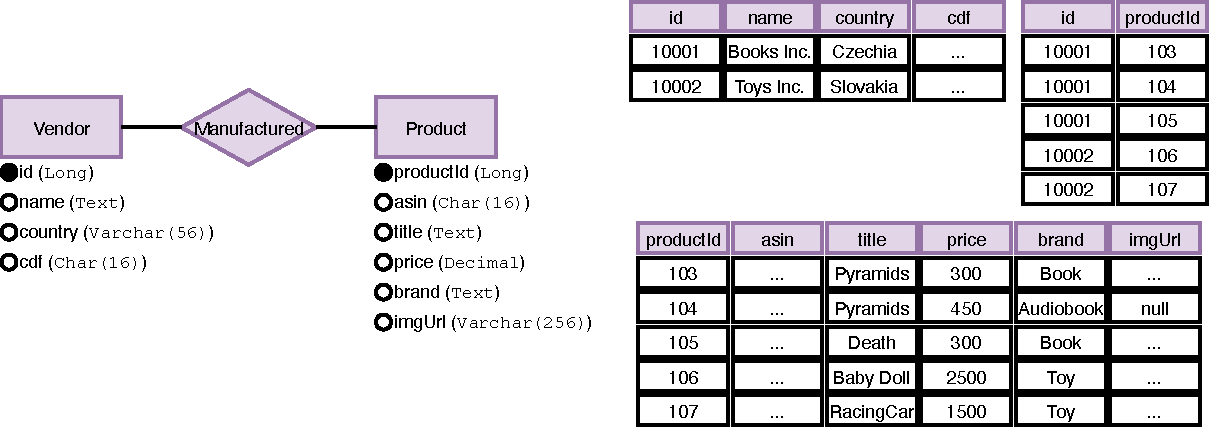
\includegraphics[scale=0.66]{img/example-relational.pdf}
\caption{An example of relational data~\cite{inference}.}
\label{fig:relationaldata}
\end{figure}

When querying relational data (typically using SQL), the largest amount of effort is generally spent on joining data together using database joins, in order to extract the data from the normalized form that it is stored in.
This is a tradeoff which many are happy to make, considering relational databases generally offer great support for Online Transactional Processing (OLTP) workloads in the form of transactions -- bundles of database commands which are executed with "all or none" semantics.
Relational systems also tend to have very good support of database integrity management tools, allowing database administrators to have full confidence in the continued integrity of their data.

However, the NoSQL movement has brought with it a desire for database \textit{horizontal scalability}, as use cases arise where simply vertically scaling a relational database system by improving its hardware is not always enough~\cite{relational_out}.
In such use cases brought on by the advent of Big Data, many are seeking to leverage the benefits of traditional relational databases in the context of scalable and highly available data.
This has spawned efforts which can be described as the NewSQL movement~\cite{newsql}.
As examples, one can look at databases like CockroachDB\footnote{\url{https://www.cockroachlabs.com/product/}} or VoltDB\footnote{\url{https://www.voltactivedata.com/}}, which offer relational databases with the speed and scalability of NoSQL systems.

For the purposes of this thesis, it is necessary to point out a few representative database system for each data model, for the purposes of developing a universal querying approach.
It would not be reasonably feasible to develop such an approach with respect to every database from each data model, therefore we simply select a couple of popular representative systems which feature the main characteristics of its corresponding data model.
For relational databases, we put forward PostgreSQL\footnote{\url{https://www.postgresql.org/}} and MySQL\footnote{\url{https://www.mysql.com/}} as some of the most popular options.

\section{Document Model}

One of the main critiques often leveraged at relational databases, especially by developers who highly value speed of development, is the fact that they can have a prohibitively high start-up cost in terms of data modeling and database management.
If speed of development and ease of reasoning about the data model are of high importance, one may soon find themselves considering document oriented databases~\cite{document_dbs}.
These databases are aggregate-oriented, with the aggregate boundaries being drawn as the boundaries of \textit{documents} -- self-contained pieces of data with a potentially complex structure.
We can think of documents in a document-oriented database in terms of objects in a programming language -- each has a structure and carries some data.
Objects in the document-oriented model generally do not need to adhere to a schema, which makes document databases popular where ease of development is paramount.
An example of document data may be seen in~\cref{fig:documentdata}.

\begin{figure}[ht]
\centering
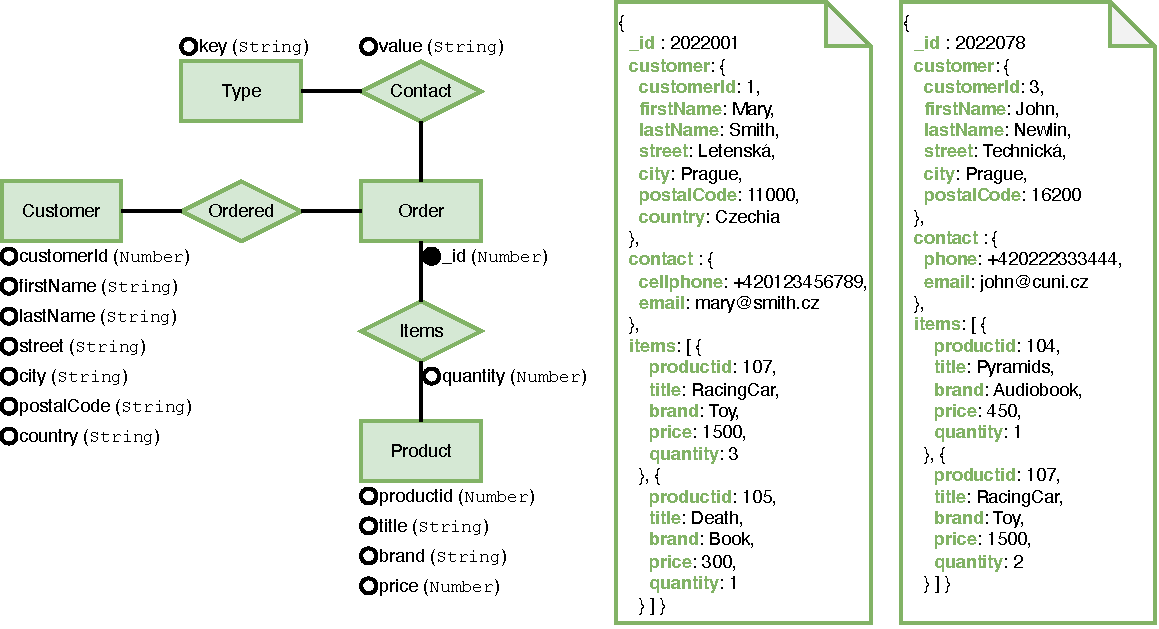
\includegraphics[scale=0.66]{img/example-json.pdf}
\caption{An example of document data in the JSON format~\cite{inference}.}
\label{fig:documentdata}
\end{figure}

Choosing a representative of the document model is not difficult, as MongoDB\footnote{\url{https://www.mongodb.com/}} is a very prominent and popular document database, which is very widely used in practice.
MongoDB organizes documents into \textit{collections}, which are sets of related documents which may be queried together.
Working with MongoDB can have a relatively user-friendly learning curve, as one can store objects from most popular programming languages into the database in JSON\footnote{\url{https://www.json.org/json-en.html}} form without too many modifications, unlike the relational model where Object-Relational Mappers (ORM) are often required.
However, in more complex use cases where working with multiple documents in a single transaction is required, developers may find the complexity resurfacing.

\section{Graph Model}

Graph databases model data in terms of objects (nodes) and relationships between those objects.
There exist two main kinds of graph models -- edge-labeled graphs and property graphs.
Both of these graph models are discussed at greater length in~\cref{querylanguages:section:graphdatamodels}.
To see an example of data in the graph model, we refer the reader to~\cref{fig:graphdata}.

\begin{figure}[h]
\centering
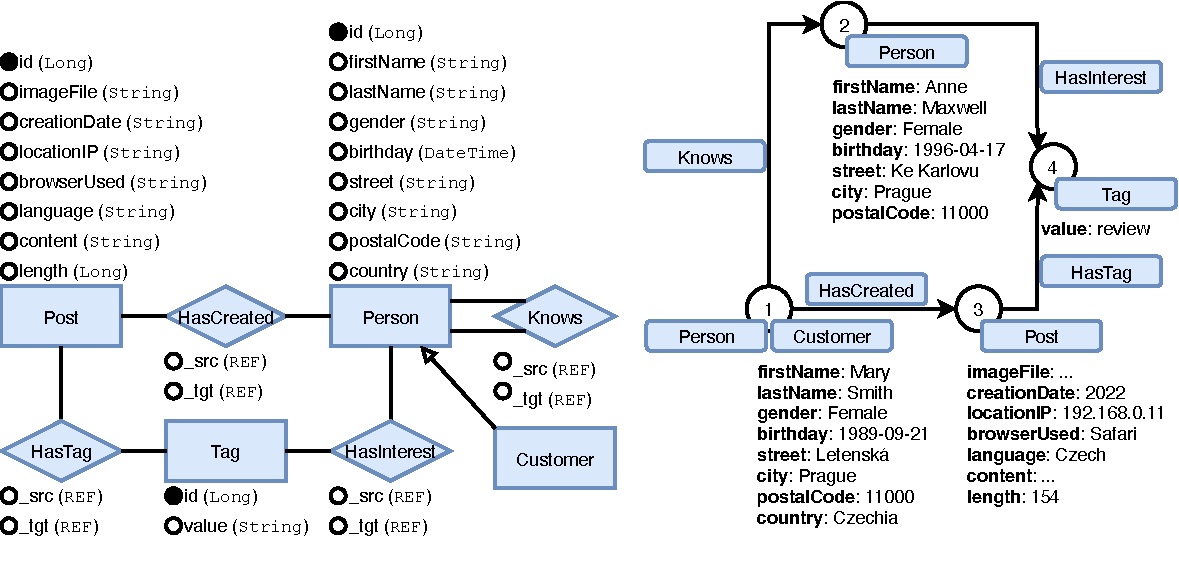
\includegraphics[scale=0.66]{img/example-graph.pdf}
\caption{An example of graph data~\cite{inference}.}
\label{fig:graphdata}
\end{figure}

In general, graph databases are best suited for use cases where the graph nature of the data is important.
These systems excel at querying for relationships between objects, and at finding patterns in the data.
Unlike relational data, relationships in graph data models are first-class entities, and may often be given properties.
In theory, graph databases provide a performance advantage compared to relational databases when considering graph-oriented workloads, however, this is not a clear-cut point of consensus in the academic community~\cite{against_graph}.

Regardless of performance implications however, it is undeniable that when presented with graph-like data, it is most convenient to model that data in a graph database.
As such, a number of graph databases have reached wide adoption today.
One of the foremost representatives of graph databases is Neo4j\footnote{\url{https://neo4j.com/}}.
Although the rest of this thesis considers Neo4j as the main representative of graph databases, a special mention should be made to RDF data which is briefly discussed in~\cref{querylanguages:subsection:edgelabeled}, as RDF is also a graph data format, and is often used in the semantic web community.

\section{Wide-Column Model}

Wide-column data may seem very similar to relational data on the surface -- both have concepts like rows and columns, storing data in table-like structures.
However, the major difference from the relational model is the fact that the names and format of the columns may differ between rows of the same table (or column family, as it is sometimes called).
Column-oriented databases store data in column-major order rather than in row-major order, meaning all values for a single column are stored contiguously, rather than contiguously storing all values for a single row.
This confers performance benefits in many cases, such as for workloads where reading all data related to a single record is rare.
An example of columnar data is shown in~\cref{fig:columnardata}.

\begin{figure}[hb]
\centering
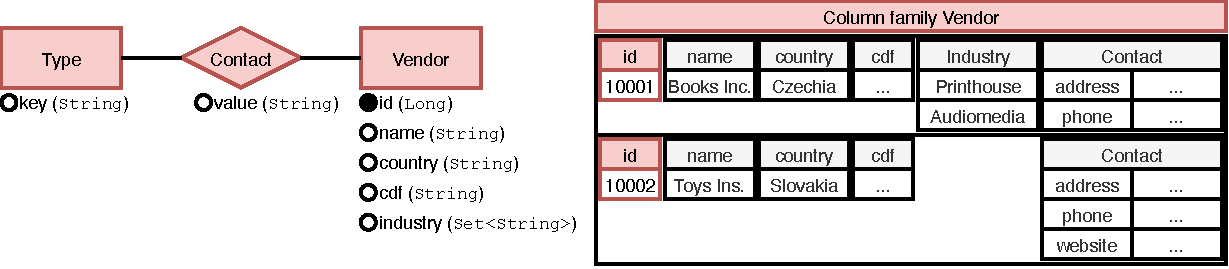
\includegraphics[scale=0.66]{img/example-columnar.pdf}
\caption{An example of columnar data~\cite{inference}.}
\label{fig:columnardata}
\end{figure}

When picking a representative for wide-column databases, Apache Cassandra\footnote{\url{https://cassandra.apache.org/_/index.html}} is a clear candidate, as it is open-source and widely used.

\section{Key-Value Model}

A key-value database or key-value store may be thought of as a hash table, which is designed to quickly store and retrieve opaque values.
As such, key-value databases are very well suited to workloads like caching, often times being used as an in-memory cache of a slower, on-disk database.
Naturally, the weakness of key-value databases is the fact that they are not generally designed to examine or query the actual values stored in any way beyond retrieving them based on the key.
Therefore, they may not be ideal for more complex transactional or analytical workloads.
See~\cref{fig:keyvaluedata} for an example of key-value data.

\begin{figure}[ht]
\centering
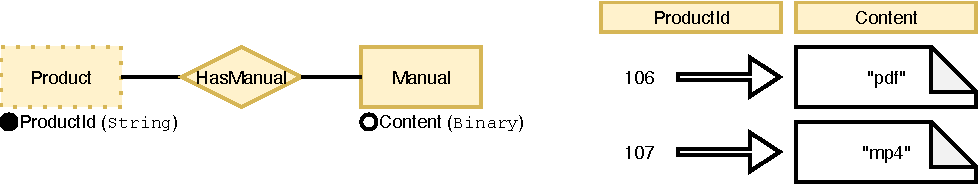
\includegraphics[scale=0.66]{img/example-keyval.pdf}
\caption{An example of key-value data~\cite{inference}.}
\label{fig:keyvaluedata}
\end{figure}

We will consider Redis\footnote{\url{https://redis.io/}} and Riak KV\footnote{\url{https://riak.com/products/riak-kv/}} as representatives of a key-value stores for the purposes of this thesis.

\chapter{Categorical Data Representation}
\label{categorical:chapter}

In the previous chapter, we examined the various data models which are widely in use today.
As we saw, there is great variety between the models, and the same thing is true for the query languages designed for their respective models.

In this chapter, we will explore a concrete unified representation~\cite{unified_representation}\cite{one_model} of multi-model data using category theory, a powerful branch of mathematics which studies mathematical structures and relations between them.
We will also discuss the benefits of such a representation, and we will then utilise it to build a universal, multi-model query language.

\section{Benefits of a Unified Representation}

As discussed in~\cref{multimodel}, there already exist two approaches to encompassing multiple data models in a single database system -- polystores~\cite{polystores}\cite{polystores2} and multi-model database systems~\cite{multimodel_dbs}\cite{multimodel_dbs2}.
However, neither approach provides a true, seamless, multi-model experience in terms of data modeling, querying and management, or this experience is only limited to two or three select models~\cite{multimodel_dbs2}.
Naturally, it would be beneficial to be able to work with all popular models in such a unified way.
Ideally, such a unified representation allows us to do the following~\cite{unified_representation}:

\begin{enumerate}
    \item capture all the existing models, preferably in the same and definitely in a standard way; 
    \item query across multiple interconnected models efficiently; 
    \item perform correct and complete evolution management, i.e., propagation of changes; 
    \item enable data migration without complex reorganisations; and 
    \item permit integration of new data models.
\end{enumerate}

Specifically, for the purposes of this thesis, having such a unified representation of multi-model data would form the perfect base for designing a multi-model query language.
This is why we will spend a short while examining the unified representation of multi-model data proposed by Martin Svoboda, Pavel Koupil and Irena Holubov{\'a}~\cite{unified_representation}\cite{one_model}.
To demonstrate the concepts that we will explain in this chapter, we present a sample multi-model scenario in~\cref{fig:datamodel}, with a corresponding Entity Relationship (ER) schema shown in~\cref{fig:erschema}. 

\begin{figure}[ht]
\centering
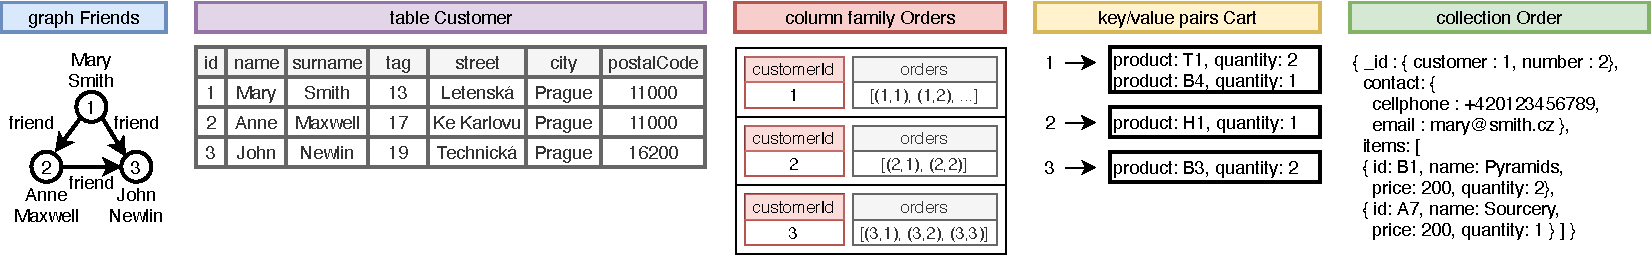
\includegraphics[width=\textwidth]{img/fig_data-models.pdf} 
\caption{A sample multi-model data scenario~\cite{unified_representation}.}
\label{fig:datamodel}
\end{figure}

\section{Basics of Category Theory}

As mentioned earlier, category theory~\cite{category_theory} is a branch of mathematics which
studies mathematical structures and relations between them.
A category $\mathbf{C} = (\mathcal{O}, \mathcal{M}, \circ)$ consists of three entities:

\begin{itemize}
    \item A class $\mathcal{O}$, whose elements are called objects. This class may also alternatively be referred to as $Obj(\mathbf{C})$.
    \item A class $\mathcal{M}$, whose elements are called morphisms, each of which has a target object and a source object. This class may also alternatively be referred to as $Hom(\mathbf{C})$.
    \item A binary operation $\circ$ called the composition over morphisms.
\end{itemize}

A useful visualization form of a category is the form of a \textit{multigraph}, with category objects forming its set of vertices and schema morphisms forming directed edges.

We represent morphisms $f \in \mathcal{M} : A \rightarrow B$, as arrows, with $A, B \in \mathcal{O}$.
We refer to object $A$ as the \textit{domain} of morphism $f$ and to object $B$ as its \textit{codomain}\footnote{The domain and codomain may also be referred to by \textit{dom} and \textit{cod}.}.
Let $f : A \rightarrow B, g : B \rightarrow C \in \mathcal{M}$ be morphisms, then the composite morphism $g \circ f \in \mathcal{M}$ is also part of the set of morphisms in the same category, also called the \textit{transitivity} property.
The morphism composition operation is not only transitive, but it is also \textit{associative}, i.e., $h \circ (g \circ f) = (h \circ g) \circ f$ for any morphisms $f, g, h \in \mathcal{M}$ such that $f : A \rightarrow B, g : B \rightarrow C$, and $h : C \rightarrow D$.
Finally, for every object $A \in \mathcal{O}$, an \textit{identity} morphism $1_A$ must exist, where $f \circ 1_A = f = 1_B \circ f$ for any $f : A \rightarrow B$.
With respect to the composition operation, this identity morphism therefore acts as a unit element.

\begin{figure}[ht]
\centering
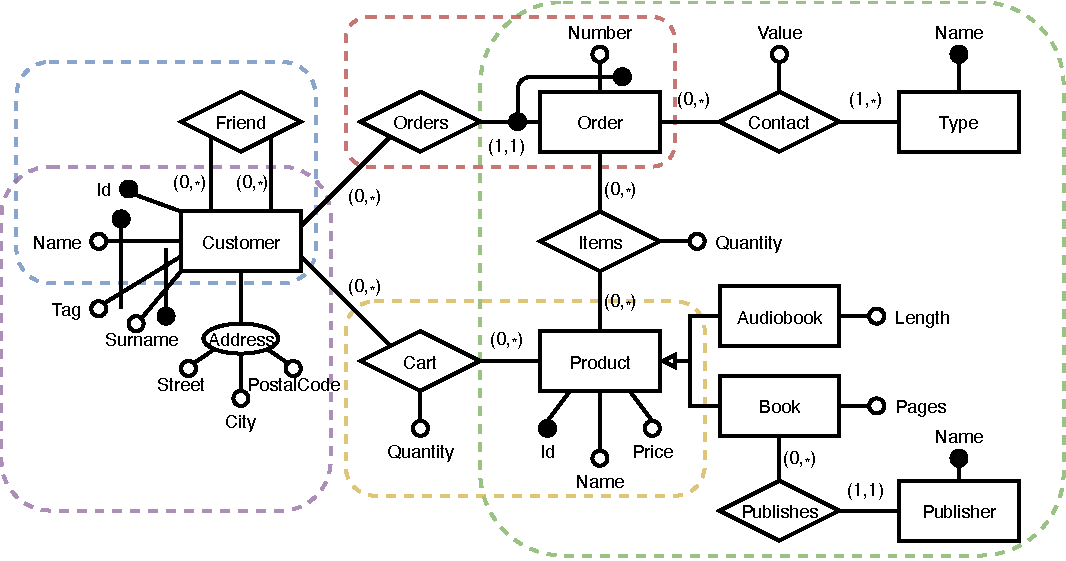
\includegraphics[width=\textwidth]{img/fig_schema-er.pdf} 
\caption{ER schema of the sample multi-model scenario in Figure~\ref{fig:datamodel}~\cite{unified_representation}.}
\label{fig:erschema}
\end{figure}

With these basic concepts from category theory, we can introduce the unified model~\cite{one_model}\cite{unified_representation} which we will be using in the rest of this thesis.
We will introduce three main concepts which together form the basis of this model -- the \textbf{schema category} describing the schema of the data in question, the \textbf{instance category} describing actual data conforming to its corresponding schema category, and the \textbf{mappings} which describe how objects from the schema category are stored in the underlying databases.
Note that the introduction of the following concepts is somewhat informal and does not cover every single aspect of the categorical model, and for this reason we refer the reader to the original sources on the matter~\cite{one_model}\cite{unified_representation} for a more comprehensive definition.

\section{Schema Category}
\label{categorical:section:schema}

We define a \textit{schema category}~\cite{one_model}\cite{unified_representation} as a tuple  $\mathbf{S} := (\mathcal{O}_\mathbf{S}, \mathcal{M}_\mathbf{S}, \circ_\mathbf{S})$, with $\mathcal{O}$ being the set of \textit{schema objects}, $\mathcal{M_\mathbf{S}}$ being the set of schema morphisms, and $\circ$ being the morphism composition operation.
Schema morphisms in $\mathcal{M}_\mathbf{S}$ connect pairs of objects from $\mathcal{O_\mathbf{S}}$.
We distinguish two types of morphisms in $\mathcal{M}_\mathbf{S}$:

\begin{itemize}
    \item \textit{Base} morphisms are morphisms which are explicitly defined; and
    \item \textit{Composite} morphisms which are obtained via the composition of base or composite morphisms via the composition operation $\circ$.
\end{itemize}

We define each schema object $o := (key$, $label$, $superid$, $ids) \in \mathcal{O}_\mathbf{S}$ to be a tuple.
Let $\mathbb{O} \subseteq \mathbb{N}$ be a set of numbers forming the set of object identifiers.
Then $key \in \mathbb{O}$ is an automatically assigned object identifier, unique for each schema object.
We can optionally define names for schema objects using the $label$ property, which is defined as $\bot$ when missing.
Naturally, we also need our schema to contain the model of the data it represents.
For this reason, each object contains a set of attributes $superid \ne \emptyset$, where each attribute corresponds to a morphism signature, introduced in the following paragraph.
The set $superid$ models the data each object is expected to contain.
Finally, the set $ids \ne \emptyset \subseteq \mathcal{P}(superid)$ is a set of identifiers, each being a set of attributes from $superid$.
This allows us to uniquely distinguish individual data instances using their attributes.

\def\myConcat{\!\cdot\!}

Each morphism $m := (signature$, $dom$, $cod$, $min$, $max) \in \mathcal{M}_\mathbf{S}$ is also defined as tuple, regardless of whether the morphism is base or composite.
Firstly, let us define the alphabet $\mathbb{M}$, and the set of possible strings $\mathbb{M}^{*}$ over this alphabet (including $\varepsilon$ which denotes an empty string).
These strings are ordered lists of symbols from $\mathbb{M}$, concatenated using the $\cdot$ operator (for example $1$ for a string containing a single character, $1.2.3$ for a string with three characters, and $\varepsilon$ for an empty string).
For a given morphism $m$, $signature \in \mathbb{M}^{*}$ uniquely identifies this morphism, save for all identity morphisms which share the $\varepsilon$ signature.
If $m$ is a base morphism, its signature will be a single alphabet symbol, i.e. $signature \in \mathbb{M}$.
If $m$ is a composite morphism however, its signature will be a string $signature \in \mathbb{M}^{*} \setminus (\mathbb{M} \cup \{\varepsilon\})$, as this allows us to decompose a composite morphism into its constituent base morphisms according to the $\circ$ operation.
The domain and codomain of $m$ are represented by $dom$ and $cod$ respectively, with both referring to schema objects in $\mathcal{O}$.
In order to model the cardinality of each morphism, we also have the properties $min \in \{\mathtt{0}, \mathtt{1}\}$ and $max \in \{\mathtt{1}, \mathtt{*}\}$, which specify the minimal and maximal number of occurrences of each specific morphism in the instance category respectively.

\begin{figure}[!htb]
\centering
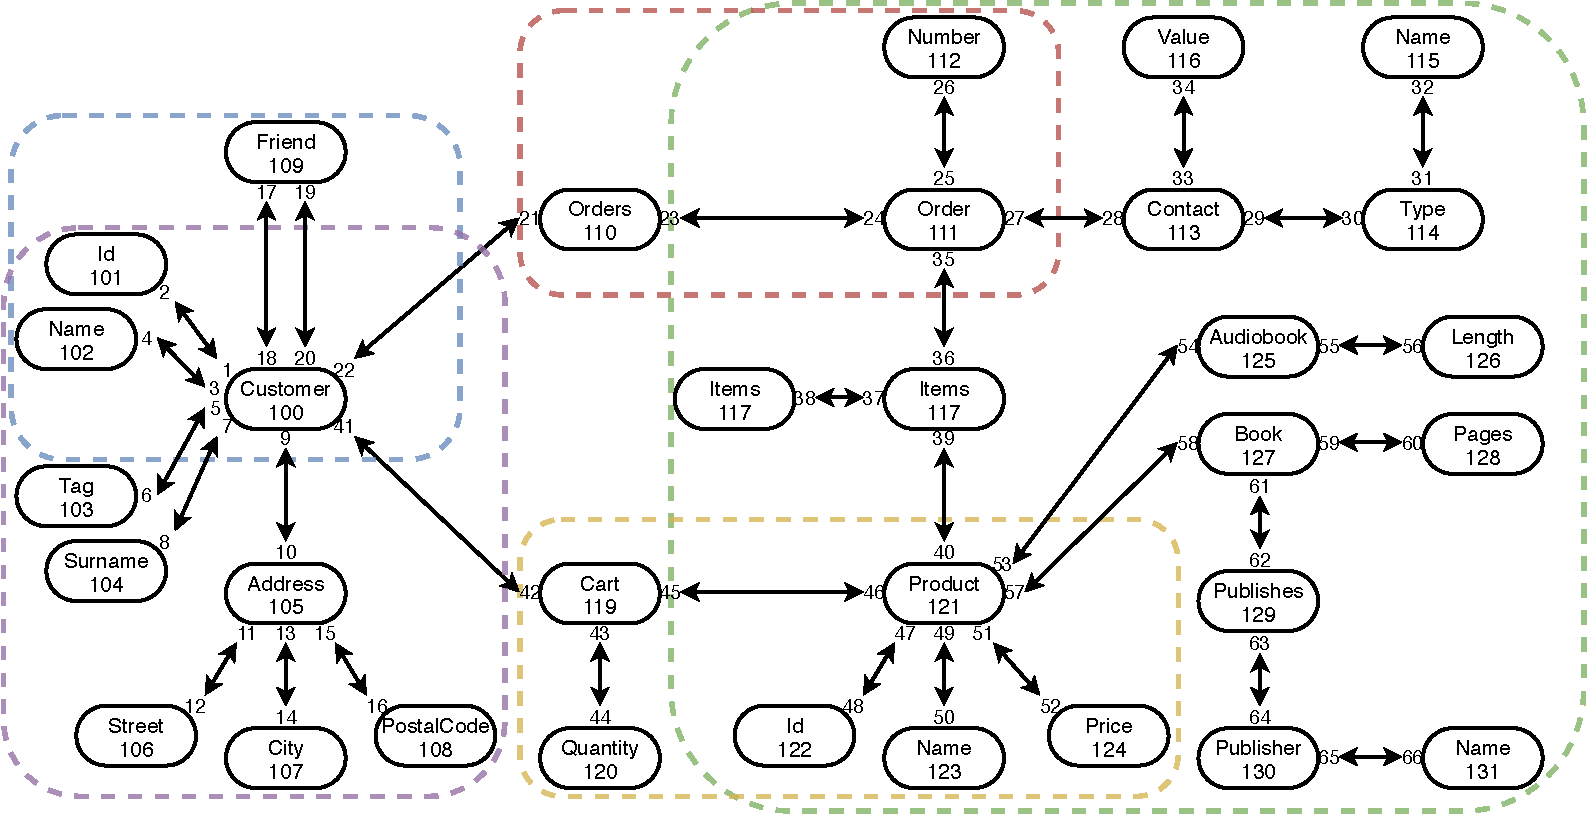
\includegraphics[width=\textwidth]{img/fig_schema-categorical.pdf} 
\caption{Schema category which was extracted from the sample ER schema in \cref{fig:erschema}~\cite{unified_representation}.}
\label{fig:schemacategory}
\end{figure}

When it comes to morphism composition, we define the signature of the composite morphism $m_2 \circ m_1$ to be $signature := signature_2\myConcat signature_1$, unless either morphism is an identity morphism, in which case the resulting signature is the signature of the other morphism.
The domain and codomain are composed naturally, resulting in the composite morphism having the domain of $m_1$ and codomain of $m_2$.
Finally, we define the composite cardinalities to be  $min = \min(min_1, min_2)$ and $max = \max(max_1, max_2)$.
With the necessary definitions out of the way, we present an example of a schema category in \cref{fig:schemacategory}, where we can see the schema category corresponding to the sample multi-model scenario presented earlier in \cref{fig:datamodel}.

\section{Instance Category}
\label{categorical:section:instance}

As we mentioned earlier, the schema category $\mathbf{S}$ only describes the schema of the data, not data instances themselves.
For this, we need to introduce the notion of an \textit{instance category}~\cite{one_model}\cite{unified_representation}.
An instance category $\mathbf{I} = (\mathcal{O}_\mathbf{I}, \mathcal{M}_\mathbf{I},$ $\circ_\mathbf{I})$ has the same structure as the corresponding schema category $\mathbf{S}$, meaning that for each schema object and morphism in $\mathbf{S}$, there exists a corresponding instance object or morphism in $\mathbf{I}$ and vice versa.
A particular instance category $\mathbf{I}$ describes the data stored in a set of databases at a particular point in time, being essentially a snapshot of the entire data set.
Whenever the underlying data changes, this will naturally induce a new instance category, with the relevant changes reflected.

Even though the sets of objects $\mathcal{O}_\mathbf{S}$ and $\mathcal{O}_\mathbf{I}$ have the same structure, just like $\mathcal{M}_\mathbf{S}$ and $\mathcal{M}_\mathbf{I}$, their representation must necessarily differ in order to be able to model the data instance.
Let $\mathbb{V}$ be a set of all possible primitive values within the data instance we are describing.
Then each instance object $o_\mathbf{I} := \{t_1, t_2, \dots, t_n\} \in \mathcal{O}_\mathbf{I}$ is a set of tuples $t_i: superid \rightarrow \mathbb{V}$ for all $i \in \mathbb{N}, 0 < i \leq n$, specifying the concrete values this instance object has in the current data instance.
The specific set of tuples defined for a particular data instance for an instance object $o_\mathbf{I} \in \mathcal{O}_\mathbf{I}$ is called the \textit{active domain} of this instance object, meaning the set of data currently bound to it.

Recall that each schema object also contains a set of identifiers $ids$, each of which uniquely identifies a particular object instance.
In an instance category, this unique identification property must hold for each $id \in ids$ for each $o_\mathbf{I} \in \mathcal{O}_\mathbf{I}$.
This means that if we project the active domain of this object to any particular identifier of this object, the number of unique tuples in the active domain must not change.

Now that we have explained the notion of instance objects when compared to schema objects, let us also introduce \textit{instance morphisms}, which act as binary relations between instance object active domains.
Let us consider an instance morphism $m_\mathbf{I} \in \mathcal{M}_\mathbf{I}$, $m_\mathbf{I} : o_1 \rightarrow o_2$ for some objects $o_1, o_2 \in \mathcal{O}_\mathbf{I}$.
Then $m_\mathbf{I} \subseteq o_1 \times o_2$, meaning that the morphism is a subset of the relation induced by the Cartesian product of $o_1$ and $o_2$ (meaning the product of their active domains).
Note that even though we define morphisms to be directed, we can traverse them in the opposite direction as they are defined as relations, which will be useful to us later.

\section{Mapping Data to the Categorical Representation}
\label{categorical:section:mapping}

In the previous sections, we defined the notion of a schema category representing the data schema, and an instance category representing the entire set of data at a particular point in time.
However, in order to be able to automatically transition between the native data model and the categorical model, we also need to know how they map to each other.
For this reason, we introduce the notion of \textit{mappings}~\cite{unified_representation}, which specify how data for one or more schema objects and morphisms are stored within a particular kind (recall \cref{table:datamodels:terms}) for a particular database.
For example, this could mean describing the structure of rows in a table in the relational model, the structure of documents in a collection in the document model, or the structure of objects and their relationships in the graph model and so on.
As it is likely that the entire schema will not fit within a single kind of a single database, it is expected that there will be multiple mappings for any given schema category, possibly even with some degree of overlap between the mappings if data redundancy is present.
These mappings may be created manually by the user using a tool like MM-evocat~\cite{evocat} which we will be working with later in this thesis, but there are also approaches which attempt to infer the mapping from the databases themselves like MM-infer~\cite{mm_infer}.
Note that sometimes, we may use the terms mapping and kind interchangeably in this thesis (especially during algorithmic descriptions), but in those cases we are always referring to the mapping which maps a given kind to its categorical representation.

% We don't consider root morphisms at all, maybe I should add some explanation for why we don't? Pavel Koupil said it was not necessary IIRC but I don't remember the reasoning.
Each of these mappings consists of a root object, denoting the root of the context of this kind within the schema category, the name of the kind which this mapping corresponds to, the source database of the kind, and finally an \textit{access path}, which describes the internal structure of the kind, and its mapping to the categorical representation.
The access path for any given kind has a tree-like structure rooted in the mapping's root object, and recursively specifies the shape of the kind.
We generally use a JSON-like representation of the access path, as shown in \cref{fig:mappings}.

\begin{figure}[ht]
\centering
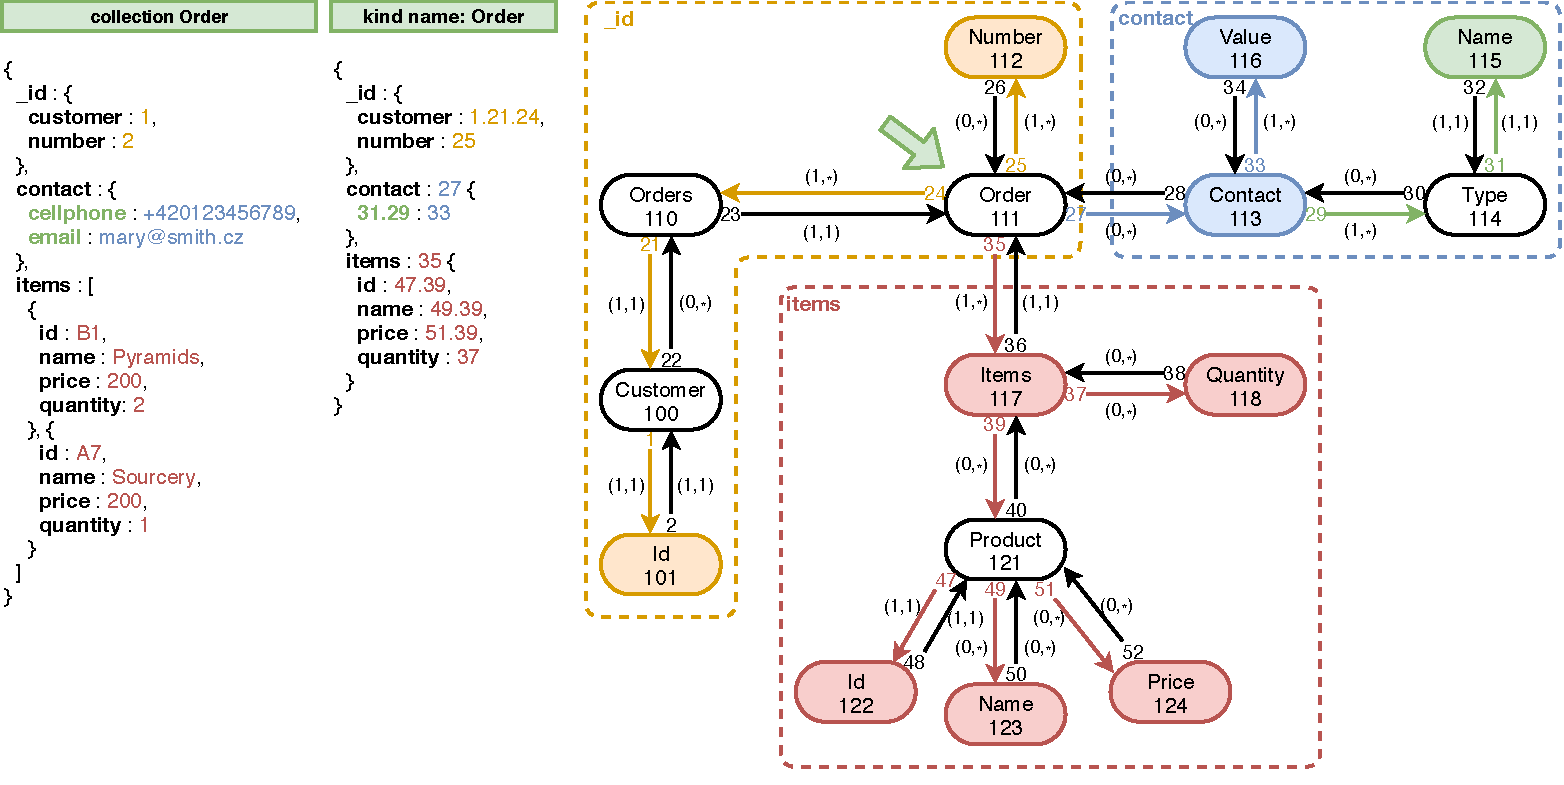
\includegraphics[width=\textwidth]{img/fig_access-path-data.pdf} 
\caption{Collection \textit{Order}, an access path for kind \textit{Order}, and the corresponding part of schema category $\mathbf{S}$~\cite{unified_representation}}
\label{fig:mappings}
\end{figure}

When defining a property within the access path, we always define its name and structure, where the structure is constrained by the particular database model (for instance, mappings for kinds in a purely relational database are always flat with no nested properties, and their property names must be unique).
This structure in the form of an access path must always cover at least one identifier of the root object, as without it, it would not be possible to distinguish different object instances.
We will point out that not every schema object needs to be the root object of a mapping, as mappings generally map the values of many schema objects which are specified within a single mapping (for example the set of customer names, surnames and ids from a single relational table).

We distinguish three possibilities for the kinds of child properties in the access path for a given mapping:

\begin{itemize}
    \item The child property is a direct neighbour of its parent in the schema category, meaning it is accessible via a base morphism.
    \item The child property is \textit{inlined} from a more distant position within the schema category, meaning it is accessible from its parent via a composite morphism. Note that multiple paths can exist in the schema category between any given objects, which is why the exact composition of the composite morphism is important.
    \item The child property is \textit{auxiliary}, meaning no corresponding object exists in the schema category. The purpose of such properties is purely structural.
\end{itemize}

The aforementioned associated morphisms are also called the property \textit{context}, as they determine which schema object each property maps to (if any).
Properties can have other kinds of names than simple static names, specifically we distinguish the following possibilities:

\begin{itemize}
    \item \textit{Static} names are user-defined as required by the structure of the underlying kind;
    \item \textit{Dynamic} names are derived from instances of particular schema objects (for example types of contact like phone or email within a customer contact object); and
    \item \textit{Anonymous} properties which do not have a name, or their naming is not permitted within the given model (for example array elements in JSON).
\end{itemize}

When it comes to the values of properties, we distinguish only two types of values:

\begin{itemize}
    \item \textit{Simple} properties which only contain primitive values; and
    \item \textit{Complex} properties containing a set or list of child properties, like a nested array or nested object in JSON. 
\end{itemize}

Note that the explanation of the concept of mappings was considerably less formal than the ones for schema and instance categories, as the formal definition is more complex in the case of mappings.
For a more formal definition of the concept of a mapping, please refer to the paper by Pavel Koupil and Irena Holubov{\'a}, where an exact definition is given~\cite{unified_representation}. 
While reading the original proposal of these ideas is not strictly necessary for readers of this thesis, it will certainly make the rest of it more digestible, as we will be expecting a certain level of familiarity with these concepts.

\section{The Need for a Categorical Query Language}
\label{category:section:querylanguage}

Now that we have examined the basics of category theory and the unified model we will be considering in the rest of this thesis, let us consider the \textit{why} of building a query language using this unified model.
As discussed earlier, there is no standard truly multi-model query language, which would be able to uniformly encompass all currently popular data models.
The utility of such a query language should be fairly apparent -- one does not need to bother with a different query language for each subset of their data which happens to be stored in a database with a different paradigm.
On the contrary, queries across the entirety of one's data may easily be expressed in the same query language.

Even in the situation where one is not particularly perturbed by the need to know multiple query languages, there are still a few more problems on the horizon.
Namely, there is an issue with queries which cross the boundaries of multiple database systems.
For example, let us consider a scenario where we store a table of user information in PostgreSQL, and we store the order information in a collection in MongoDB.
In such a case, expressing a query which crosses the boundaries of both databases is impossible without sharing the same query language.

As the reader now hopefully shares our enthusiasm for the existence of such a language, we must still formalize the requirements for such a language.
This language should:

\begin{itemize}
    \item be able to encompass the particulars of all popular data models,
    \item be able to express queries crossing model boundaries,
    \item be expressive and readable,
    \item leverage the power of category theory,
    \item be intuitive and familiar to users of existing query languages,
    \item have the capability of being nearly as performant as native queries where possible.
\end{itemize}

Considering we may look at a category as a multigraph, we may not need to create a categorical query language from scratch.
We can attempt to take inspiration in existing graph query languages, which is the focus of the following chapter.

\chapter{Existing Graph Query Languages}
\label{querylanguages}

Before engaging in the endeavor of designing a brand new graph query language for the categorical representation described in the previous chapter, it is prudent to first analyze other existing graph query languages, and consider their features, advantages and disadvantages. The most popular graph query languages are SPARQL~\cite{sparql}, Cypher~\cite{opencypher}, Gremlin~\cite{gremlin} and PGQL~\cite{pgql}.
Another language worth mentioning is G-CORE~\cite{gcore}, a graph query language designed by a team of academics and industry professionals, although it does not currently have an implementation.
This chapter explores the properties of these languages and attempts to make a comparison of their capabilities.

\section{Graph Data Models}
\label{querylanguages:section:graphdatamodels}

Graph data can be modeled in a variety of ways, and each data model will naturally require a different kind of query language, despite containing only graph data.
As such, a proper analysis of existing graph query languages necessitates a formalization of these data models.
Naturally, a number of different graph data models have been tried in practice, but two have emerged as the most commonly used: \textit{edge-labeled graphs} and \textit{property graphs}, as described by Angles et al.~\cite{foundations_query_languages}
All of the aforementioned graph query languages operate on one of these two data models.

This section does not provide a rigorous definition of these data models, as their details may vary slightly between databases and query languages.
Instead, it aims to illustrate the concepts of each data model and to showcase how they model data.
As an aside, all graphs are implied to be directed multigraphs consisting of a set of vertices and a set of edges, unless explicitly specified otherwise.

\subsection{Edge-Labeled Graphs}
\label{querylanguages:subsection:edgelabeled}

Edge-labeled graphs are graphs which assign a label to each edge from a set of labels.
Each edge has exactly one label, while vertices are unlabeled.

This data model is quite simple yet strong.
A vertex with a property can be modeled by introducing a new vertex containing the property value and connecting it with the original vertex via an edge labeled with the property name.
Similarly, it is possible to model labeled vertices by introducing a new vertex containing the vertex label value, and connecting it with the original vertex via an edge labeled with an arbitrarily defined label, selected to denote vertex labels.
The edge-labeled graph model is also capable of representing edge properties.
This can be achieved by reification - materializing the edge into an extra vertex connected with new edges to both ends of the original edge.
The extra vertex can then be linked with additional edges to other vertices representing the property values.
An example of data modeled as an edge-labeled graph may be seen in~\Cref{fig:edgegraph}.

\begin{figure}[ht]
\centerline{\mbox{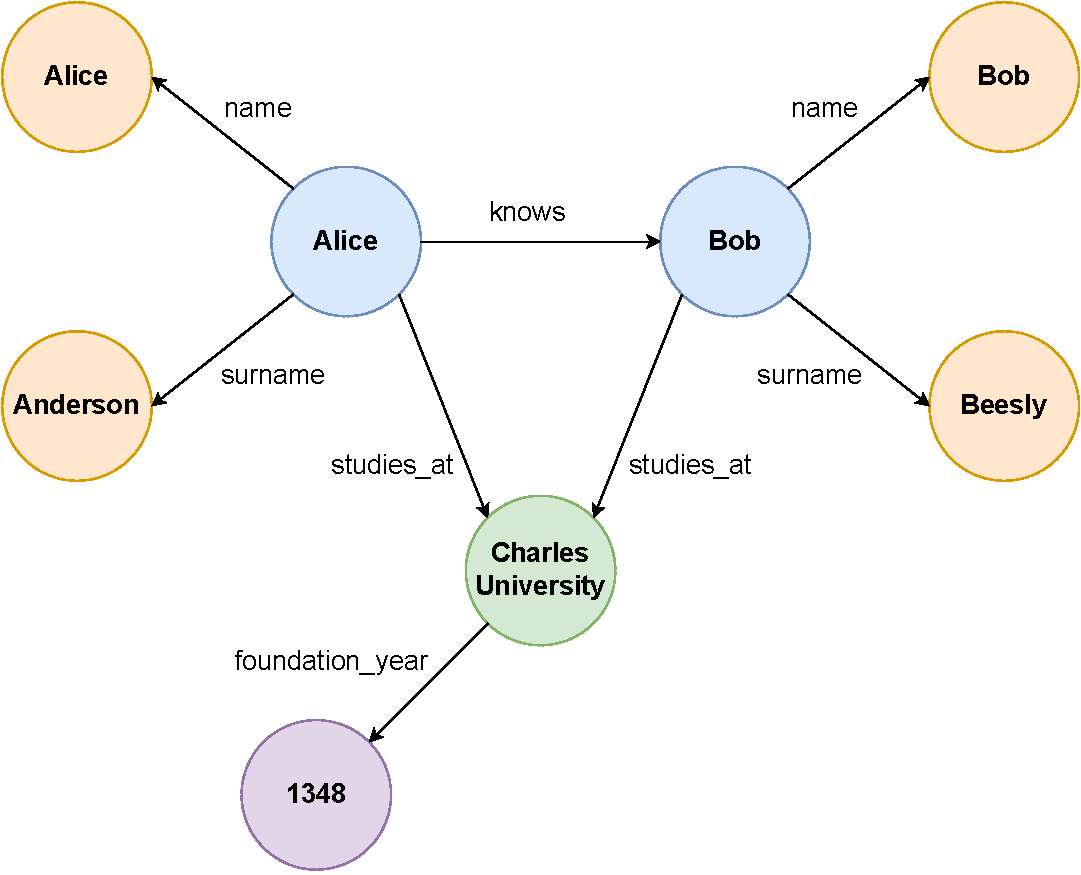
\includegraphics[width=0.8\textwidth]{img/edge-labeled-graph.pdf}}}
\caption{Data modeled as an edge-labeled graph.}
\label{fig:edgegraph}
\end{figure}

Edge-labeled graphs are the data model for the Resource Description Framework~(RDF)~\cite{rdf}, for which SPARQL~\cite{sparql} acts as the most popular query language.
RDF is a framework for representing information on the Web, and it models information as triples in the form \textit{subject predicate object}.
RDF graphs may contain three types of nodes: Internationalized Resource Identifiers~(IRIs), literals (value types like strings and numbers) and blank nodes (vertices without a globally persistent IRI).
Predicates are always IRIs, which can be equated to edges with labels from edge-labeled graphs.

\subsection{Property Graphs}

A graph data model used more widely in practice by graph-oriented databases is the property graph.
A property graph can be seen as an extension of edge-labeled graphs, where both vertices and edges may be labeled.
In addition, each vertex and edge may be associated with a set of key-value pairs called \textit{attributes}, which store additional information about the vertex or edge.
An example of data modeled as a property graph can be seen in~\cref{fig:propgraph}.

\begin{figure}[ht]
\centerline{\mbox{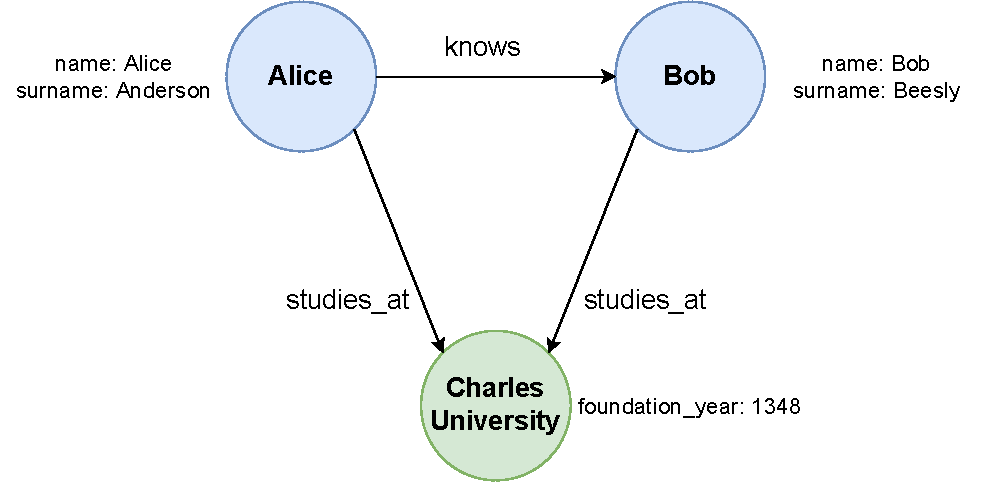
\includegraphics[width=0.8\textwidth]{img/property-graph.pdf}}}
\caption{Data modeled as a property graph.}
\label{fig:propgraph}
\end{figure}

These additional constructs do not give property graphs a higher expressive power compared to edge-labeled graphs, but they do carry other benefits.
First of all, the structure of the data in property graphs may be easier for users to work with, since data related to a particular vertex or edge is associated directly with that vertex or edge, rather than residing in a different vertex.
Additionally, imagine a scenario where we have an edge-labeled graph, and we need to add a property to an edge which previously did not have any properties.
The solution to this problem is to use reification and create a new in-between vertex holding the new property.
However, such a change is disruptive to the schema of the data, and will necessarily break existing queries.
Using the property graph model, such a change can be done without significantly disrupting the schema.

The property graph  model forms the basis for the majority of modern graph data platforms.
The foremost among them are Neo4j\footnote{\url{https://neo4j.com/}} and Apache TinkerPop\footnote{\url{https://tinkerpop.apache.org/}}, which primarily allow querying with Cypher~\cite{opencypher} and Gremlin~\cite{gremlin} respectively.

\section{Language Features}

With the graph data models clarified, we analyze the specifics of each selected graph query language.
The presented languages are a sample of the most popular graph query languages which cover a variety of concepts and problem domains.
% Maybe I should write another paragraph about the most important features and their explanations? Something like 'joins and unions and projections exist, what is composability etc
Specifically, this section focuses on the querying capabilities of the given languages, and only briefly covers their mutation functionality.

\subsection{SPARQL}
\label{querylanguages:subsection:sparql}

As SPARQL~\cite{sparql} is primarily used as the query language for RDF~\cite{rdf}, it is different from the other selected query languages in that it operates on an edge-labeled graph.
It operates in terms of triple patterns~--~whitespace-separated lists consisting of a subject, predicate, and object.
Any part of the triple pattern may consist of a constant (IRI or RDF literals like strings and numbers) or a variable.
These triple patterns can then be used to match parts of the queried graph.
SPARQL itself only supports querying, but SPARQL 1.1 Update~\cite{sparql_update}, which is an update language for RDF graphs, allows for updates with a syntax very similar to SPARQL.

\begin{figure}[ht]
\begin{code}[]
PREFIX lib: <http://example.org/library#>

SELECT ?author ?book
WHERE
{
    ?author lib:authored    ?book .
    ?book   lib:releaseYear 2015  .
    ?author lib:birthYear   ?authorBirthYear .
}
ORDER BY ASC(?authorBirthYear)
\end{code}
\caption{Basic SPARQL query example.}
\label{fig:sparqlbasic}
\end{figure}

A simple SPARQL query which retrieves a list of books released in 2015 and their respective authors (ordered by birth year) may be seen in \Cref{fig:sparqlbasic}.
It can be seen that the SPARQL query structure is in some ways inspired by SQL~--~we have a \texttt{SELECT} clause specifying what the query should return, as well as a \texttt{WHERE} clause specifying the conditions for the returned variables, and an \texttt{ORDER BY} clause.
However, these similarities end upon inspection of the graph querying capabilities of SPARQL.
In order for a set of variable bindings to be returned by the query, their substitution into the \texttt{WHERE} clause must induce a valid subgraph of the queried graph.
This \texttt{WHERE} clause utilizes the aforementioned triple patterns to this end.
In the sample query, the first triple pattern specifies that the query should match triples in the form of \texttt{?author lib:authored ?book .}, where the dot at the end signifies the end of the triple.
The second triple specifies that the matched book should be released in 2015.
Specifying both triples after one another in the \texttt{WHERE} clause functions as their conjunction - both must match in order for the entire \texttt{WHERE} clause to match.
Lastly, the \texttt{PREFIX} clause simply specifies the prefix \texttt{lib:} to be equivalent to the namespace IRI \texttt{http://example.org/library\#}.
This does not increase the expressive power of SPARQL, but it makes queries significantly more readable compared to queries which use the full namespace IRI at every occurrence.

SPARQL also supports more complex graph patterns such as joins, unions, differences, optional matching, and filtering.
Joins are implicit both between triple patterns and graph patterns -- they act as a natural join on the set of shared variables between the two patterns whenever they are specified within the same graph pattern.
The \texttt{MINUS} and \texttt{NOT EXISTS} expressions allow the elimination of matches depending on the evaluation of a pattern and the existence of a pattern respectively.
Using the \texttt{OPTIONAL} keyword, the query may specify that parts of the graph pattern are optional, meaning that when they cannot be successfully matched for a given solution, that solution is not discarded, but rather any unmatched variables remain unbound.
Filtering matches are possible using the \texttt{FILTER} keyword, which specifies a condition and filters all matches which do not satisfy this condition.

\begin{figure}[ht]
\begin{code}[]
PREFIX lib: <http://example.org/library#>

SELECT ?author ?book ?rating
WHERE
{
    { ?author lib:authored ?book . }
    UNION
    { ?author lib:coauthored ?book .}
    
    ?book   lib:releaseYear ?releaseYear .
    OPTIONAL { ?book lib:rating ?rating . }
    
    FILTER(?releaseYear >= 2015)
}
\end{code}
\caption{More complex graph pattern matching in a SPARQL query.}
\label{fig:sparqlpattern}
\end{figure}

More complex graph pattern matching can be seen in \Cref{fig:sparqlpattern}.
This query returns the list of authors and co-authors of books which have been released in  2015 or later, and additionally returns the book rating if it is available.
If the rating is not present in the data, that book is still returned, with the \texttt{?rating} variable remaining unbound.
The \texttt{UNION} construct in the query ensures that results will be returned for both authors and co-authors of any given book.

When it comes to navigational queries (i.e. queries which navigate the graph), SPARQL uses the concept of \textit{property paths}.
These are constructs not unlike regular expressions, which specify possible routes through a graph between two graph nodes.
Property paths may contain RDF terms or variables at both ends, but they cannot contain variables as part of the path itself.
An example of a property path is \texttt{lib:TheHobbit lib:sequel+ ?book .}, which will bind the \texttt{?book} variable to any book which follows The Hobbit as a direct or indirect sequel.
A path like \texttt{lib:TheHobbit lib:sequel/lib:rating ?rating .} would bind \texttt{?rating} to the rating of The Hobbit's direct sequel.
Additional property path features include inverse paths from object to subject, alternative paths or negated property sets which match any except the specified IRIs in the path.

\Cref{fig:sparqlnav} shows a query which returns the list of all authors who co-authored a book with J. R. R. Tolkien.
This query uses a property path to find all books co-authored by Tolkien, and then uses an inverse path from these books to their co-authors.
Note that it is necessary to filter Tolkien himself from the results of the query, as the \texttt{?author} variable would otherwise match Tolkien himself, as he is naturally a co-author for all books he co-authored.

\begin{figure}[ht]
\begin{code}[]
PREFIX lib: <http://example.org/library#>

SELECT DISTINCT ?author
WHERE
{
    lib:JRRTolkien lib:coauthored/^lib:coauthored ?author .
    FILTER(?author != lib:JRRTolkien) .
}
\end{code}
\caption{Graph navigation in a SPARQL query.}
\label{fig:sparqlnav}
\end{figure}

SPARQL is most notably supported by the Virtuoso\footnote{\url{https://virtuoso.openlinksw.com/}}, Amazon Neptune\footnote{\url{https://aws.amazon.com/neptune/}}, Stardog\footnote{\url{https://www.stardog.com/}}, Apache Jena Fuseki\footnote{\url{https://jena.apache.org/documentation/fuseki2/}} or GraphDB\footnote{\url{https://graphdb.ontotext.com/}} graph databases.

\subsection{Cypher}

Cypher~\cite{opencypher} is a declarative graph query language originally developed by Neo4j.
It was open-sourced in 2015 and contributed to the openCypher~\cite{opencypher} project, which is now responsible for maintaining the language.
Cypher operates on a property graph data model, referring to the vertices of the graph as \textit{nodes} and the edges as \textit{relationships}.
Its structure is inspired by SQL, as queries are composed of various clauses.
Its pattern matching is also inspired by SPARQL~\cite{sparql}.
Cypher may be used for both querying and updating graphs.

Clauses in a Cypher query are chained together, and the results of each clause become the inputs for the next clause.
Regarding basic graph pattern matching, Cypher notation tries to be very intuitive when it comes to the underlying graph data model.
It models relationships as an arrow between two nodes: \texttt{(a)-[r]->(b)}.
Such a pattern describes a directed relationship \texttt{r} from the node \texttt{a} to the node \texttt{b}.
Note that both nodes and relationships do not have to be named, they may simply use the \texttt{()} and \texttt{[]} notation respectively.
The pattern \texttt{(a)-[]-(b)} will match the relationship in either direction.
These patterns are used in the \texttt{MATCH} clause, which matches the patterns to the underlying data and binds any variables accordingly.

It should be noted that unlike SPARQL, Cypher does not return matches where the same graph relationship is found multiple times in a single pattern.
What this means is that if we specify a pattern like \texttt{(a)-[]->(b)<-[]-(c)}, Cypher implicitly makes sure that the node \texttt{a} is distinct from the node \texttt{c}.
If allowing the return of the same node in different parts of the pattern is desirable, multiple consecutive \texttt{MATCH} clauses must be used, matching parts of the pattern separately and using some common variables to join them together.

\begin{figure}[ht]
\begin{code}[]
MATCH (author:Author) -[:AUTHORED]-> (book:Book {releaseYear: 2015})
RETURN author, book
ORDER BY author.birthYear ASC
\end{code}
\caption{Basic Cypher query example.}
\label{fig:cypherbasic}
\end{figure}

The last information needed for composing a simple query is knowing how to specify labels and properties.
The construct \texttt{(a:Author {surname: "Tolkien"})} \texttt{-[r:AUTHORED]->} \texttt{(b)} will match \texttt{a} to nodes labeled \texttt{Author} and with the property \texttt{surname} equal to "Tolkien", and \texttt{r} to relationships typed \texttt{AUTHORED}.
The query shown in \Cref{fig:cypherbasic} uses these principles to return a list of books released in 2015 and their respective authors (ordered by birth year).
The \texttt{RETURN} clause is used for projection on the output variables, and it is mandatory in queries which do not mutate the underlying dataset.
The \texttt{ORDER BY} clause works similarly to SQL.

Much like SPARQL pattern matching, joins happen implicitly when we specify multiple \texttt{MATCH} clauses in succession.
The \texttt{NOT} operator acts as a difference -- its usage in a \texttt{WHERE} clause after a \texttt{MATCH} clause will eliminate matching results from the results of the \texttt{MATCH} clause.
Optional pattern matching is also supported with the \texttt{OPTIONAL MATCH} clause.
Filtering is accomplished with the \texttt{WHERE} clause.

\begin{figure}[ht]
\begin{code}[]
MATCH (author:Author) -[:AUTHORED]-> (book:Book)
OPTIONAL MATCH (book) -[:RATING]-> (rating:Rating)
WHERE book.releaseYear >= 2015
RETURN author, book, rating.average AS rating

UNION

MATCH (author:Author) -[:COAUTHORED]-> (book:Book)
OPTIONAL MATCH (book) -[:RATING]-> (rating:Rating)
WHERE book.releaseYear >= 2015
RETURN author, book, rating.average AS rating
\end{code}
\caption{More complex graph pattern matching in a Cypher query.}
\label{fig:cypherpattern}
\end{figure}

\Cref{fig:cypherpattern} shows a more complex example of graph pattern matching using some of the features mentioned above.
The depicted query returns the list of authors and co-authors of books released in the year 2015 or later, and additionally returns the book rating if it is available (for simplicity's sake, we assume that the rating is stored in a node connected to a book via the \texttt{RATING} relationship).
It should be noted that Cypher does not have an easy way of specifying alternate matches like SPARQL does, and the \texttt{UNION} clause works at the level of query results.
Therefore we need to run both queries independently, and then \texttt{UNION} their results.
Cypher also does not yet support post-union processing, so if we wanted to order the results of the union, we would need to resort to other workarounds.

As far as navigational queries go, the strength of Cypher is considerably lower than that of SPARQL.
Traversal of a path is limited to a single relationship type (i.e. label), and if multiple labels are desired, the traversal has to be broken up into multiple parts.
The same applies to properties of the relationship -- path pattern matching is only able to match the same set of properties and property values for each relationship in the path.
Variable-length pattern matching is signified by the usage of the \texttt{*} operator.
The pattern \texttt{(a)-[*2]->(b)} is equivalent to the pattern \texttt{(a)-[]->()-[]->(b)},
i.e. a path of length 2.
The length of this path can be variable: \texttt{(a)-[*2..4]->(b)} means that the path is at least of length 2 but no more than length 4.
Either of these bounds can be omitted, meaning \textit{length X or more} or \textit{length X or less}.
If both bounds are omitted, the path can be of any length: \texttt{(a)-[*]->(b)}, as the lower and upper bounds default to 1 and infinity respectively.
The ability to specify a range for the path length present in Cypher is not present in SPARQL.

What Cypher lacks in terms of path traversal specification, it makes up for in other ways of working with paths.
It features paths as a first-class citizen of the language, offering the ability to save paths to variables or to return them from queries.
It also has a number of interesting functions like searching for one or all shortest paths between two nodes in the graph.
Cypher also has native support for list primitives, something which is missing from SPARQL (and RDF).

\begin{figure}[ht]
\begin{code}[]
MATCH path = (:Book {title: "The Hobbit"}) -[*:SEQUEL]-> (book:Book)
RETURN book.title AS title, length(path) + 1 AS seriesNumber
\end{code}
\caption{Graph navigation in a Cypher query.}
\label{fig:cyphernav}
\end{figure}

\Cref{fig:cyphernav} demonstrates a query which returns the list of all sequels of the book The Hobbit transitively.
The query also returns for each book its number in the series, meaning The Hobbit's direct sequel will have the number 2, its sequel the number 3 and so on.

The most notable databases using Cypher are Neo4j\footnote{\url{https://neo4j.com/}}, Amazon Neptune\footnote{\url{https://aws.amazon.com/neptune/}}, Memgraph\footnote{\url{https://memgraph.com/}}, Katana Graph\footnote{\url{https://katanagraph.com/}} and RedisGraph\footnote{\url{https://redis.io/docs/stack/graph/}}.

\subsection{Gremlin}

Gremlin~\cite{gremlin} is a graph traversal language operating on property graphs.
It was developed by Apache TinkerPop of the Apache Software Foundation, and is available under the Apache License 2.0.
Gremlin is a functional language which operates in terms of a data flow.
A traversal in Gremlin consists of a sequence of steps, each of which performs an operation on the underlying stream of data.
This data is functionally passed between three kinds of steps: map steps which transform the data, filter steps which filter, and remove some of the data, and side effect steps which can compute statistics about the data stream.

\begin{figure}[ht]
\begin{code}[]
g.V().
    hasLabel('Book').
    has('releaseYear', 2015).
    as('book').
    
    in('authored').

    hasLabel('Author').
    as('author').

    select('book', 'author').
        by('title').
        by('name')
\end{code}
\caption{Basic Gremlin query example with imperative traversal.}
\label{fig:gremlinbasic}
\end{figure}

\Cref{fig:gremlinbasic} shows a simple Gremlin query which retrieves the list of books released in 2015 and their respective authors, returning their titles and names.
The \texttt{g.V()} step returns a list of all vertices in the graph.
Using \texttt{hasLabel('Book')}, only vertices with the Book label are selected.
Similarly, the \texttt{has()} step filters out books which were not released in 2015.
The \texttt{as()} step is not a real step, but rather a step modulator which assigns a label to the previous step, making it accessible by later steps.
It can be thought of as referencing to that step with a variable.
Edge traversal is performed with the \texttt{in()} step, which in the example traverses incoming edges with the \texttt{authored} label.
Other edge traversal steps exist which traverse edges in a specified direction, or both.
The \texttt{select()} step takes data from previously labeled steps and collects them, additionally projecting the data to the book title and author name.

Gremlin differs from the previously mentioned graph query languages by allowing imperative graph traversal as shown in \Cref{fig:gremlinbasic}, but it also supports declarative traversals, as well as allowing mixing of imperative and declarative traversals.
An example of a declarative traversal can be seen in \Cref{fig:gremlinpattern}.
While declarative pattern matching is possible, it is considerably less succinct than its SPARQL or Cypher equivalents, as Gremlin focuses primarily on graph traversal.
Gremlin also supports filtering and unions, but other more complex operation like set differences and optional matching require extra effort.

\begin{figure}[ht]
\begin{code}[]
g.V().
    match(
        as('tolkien').
            hasLabel('Author').
            has('name', 'J. R. R. Tolkien'),
        as('tolkien').
            out('coauthored').
            as('book'),
        as('book').
            in('coauthored').
            as('coauthor'),
        where('coauthor', neq('tolkien'))
    ).
    select('coauthor').by('name')
\end{code}
\caption{Declarative graph pattern matching in a Gremlin query.}
\label{fig:gremlinpattern}
\end{figure}

Gremlin supports variable-length paths via the \texttt{repeat()} step, which offers both do-while and while-do semantics.
The \texttt{repeat()} step may repeat any traversal, meaning the repeated traversal may itself consist of multiple steps.
\Cref{fig:gremlinnav} showcases this in a query which performs a full traversal of the graph by iteratively following edges.
This traversal starts with the author J. R. R. Tolkien, and follows outgoing edges until it gets to end nodes which have no outgoing edges.
It uses the \texttt{simplePath()} step to eliminate any potential cycles in the graph during traversal.
It also contains another stop condition -- the maximum traversal depth of 10 set with \texttt{loops().is(10)}.
Gremlin is also able to return entire paths from a query.

\begin{figure}[ht]
\begin{code}[]
g.V().
    hasLabel('Author').
    has('name', 'J. R. R. Tolkien').
    
    repeat(out().simplePath()).
        until(outE().count().is(0).
            or().loops().is(10))
\end{code}
\caption{Graph navigation in a Gremlin query.}
\label{fig:gremlinnav}
\end{figure}

Gremlin can be used for both Online Transaction Processing (OLTP) and Online Analytical Processing (OLAP), meaning a Gremlin traversal can be executed as either a real-time database query, or as a batch analytics query.
Notable graph databases implementing Gremlin are Amazon Neptune\footnote{\url{https://aws.amazon.com/neptune/}}, OrientDB\footnote{\url{https://orientdb.org/}}, Blazegraph\footnote{\url{https://blazegraph.com/}} and Titan\footnote{\url{https://titan.thinkaurelius.com/}}.


% These chapters explain what I have designed (language, algorithms)
\chapter{MMQL -- A Categorical Query Language}
\label{mmql}

So far, we have examined the particulars of multi-model data, introduced a categorical model for representing said data, and we have formulated the need for a query language to query this model.
Based on requirements specified in~\cref{category:section:querylanguage}, this chapter introduces the \textbf{Multi-Model Query Language (MMQL)}, a query language created specifically to query the aforementioned categorical representation.
Before we introduce MMQL, the reader may get a taste of the language by examining the example query shown in~\cref{mmql:figure:example}.

\begin{figure}[ht]
\begin{code}
SELECT {
    ?customer ordered ?productName ;
        name ?customerName .
}
WHERE {
    ?product 49 ?productName ;
        -39/36 ?order .
    
    ?order -23/21 ?customer .
    ?customer 3 ?customerName .

    FILTER(?productName = "Lord of the Rings")
}
\end{code}
\caption{An example query in MMQL, retrieving customers who ordered the Lord of the Rings book. The corresponding schema category is shown in~\cref{fig:schemacategory}.}\label{mmql:figure:example}
\end{figure}

MMQL is a query language for categorical data which operates on a schema category.
Its purpose is to query data in a unified way using the categorical representation, again utilizing categorical data representation to return the data in a unified representation.
As such, if data stored across a variety of different databases is modeled using a schema category, one can query all of that data using a single, unified query language.
Under the covers, this singular query is translated into potentially many subqueries in the relevant databases' own query languages, and the results of those queries are joined to create the final query result.
We should note that MMQL is a querying-only language, it does not aspire to handle any data modifications.

Designing a query language is no trivial task, therefore this chapter pays special attention to the design process behind MMQL, and various key decisions made during its design.
This chapter explores the major concepts in MMQL, but its full grammar is available in \cref{attachment:grammar}.
A comparison of constructs supported in MMQL is shown in~\cref{tab:MM-sparql}, where we show a feature comparison with selected popular query languages, which are used in some of the most popular databases in their respective models (as we discussed in \cref{multimodel}).

\begin{scriptsize}
\begin{table}[h]
\caption{Comparison of constructs supported in MMQL and in single-model query languages~\cite{mm_quecat}.}
\label{tab:MM-sparql}
\def\arraystretch{1.2}
\begin{tabular}{
%|l|llll|
%|
    >{\raggedright\arraybackslash}p{23.9mm}
    |
    >{\raggedright\arraybackslash}p{24.9mm}
    >{\raggedright\arraybackslash}p{23.9mm}
    %>{\raggedright\arraybackslash}p{13.0mm}
    >{\raggedright\arraybackslash}p{25.9mm}
    >{\raggedright\arraybackslash}p{23.9mm}
%    |
    }

% \begin{tabular}{|l|l%l
% ll%l
% ll|}
\toprule
\textbf{MMQL}  & \textbf{PostgreSQL (SQL)}  & \textbf{Neo4j (Cypher)}  & \textbf{MongoDB}  & \textbf{Cassandra (CQL)} \\
% \hline
% MMQL         & SQL                 %& AFL (SciDB)
% & Cypher                  %& SPARQL              %& Solr (RiakKV)  
% & MongoDB              & CQL (Cassandra)    \\
\midrule
%Data source
FROM & FROM                %& project\#1
& -            %& FROM                %& bucket specification 
& db.collection       & FROM               \\
%Projection
SELECT & SELECT              %& project
& RETURN                  %& SELECT              %& fl             
& \$project & SELECT             \\
%Selection
WHERE & WHERE               %& filter
& WHERE                   %& FILTER              %& fq             
& \$match   & WHERE              \\
%Filtering
FILTER & condition(s) & condition(s) & condition(s) & condition(s) \\ %% FILTER u nás
%Aggregation
COUNT, MIN, MAX, AVG & GROUP BY ... HAVING %& aggregate
& COUNT, MIN, MAX, AVG %& GROUP BY ... HAVING %& MapReduce      
& aggregate(...)       & GROUP BY           \\
%Join/traversal
graph pattern & JOIN & MATCH & \$lookup & - \\
% Join             &  JOIN        %&  (cross\_)join
% &  -                   %&  -\#5            %&  link walking    
% &  \$lookup            &  -               \\
% Graph traversal       &  JOIN           %&  (cross\_)join
% &  MATCH                  %&  graph pattern     %&  link walking    
% &  -                   &  -               \\
% Unbounded traversal    &  WITH RECURSIVE %&  -                  
% &  MATCH with *                %&  graph pattern     %&  -               
% &  -                   &  -               \\
% Optional
OPTIONAL             &  OUTER JOIN     %&  -                  
&  OPTIONAL MATCH         %&  OPTIONAL         %&  rq (re-ranking) 
&  -                   &  -               \\
%Union
UNION &  UNION          %&  merge              
&  UNION                  %&  UNION            %&  OR              
&  \$unionWith         &  -               \\
%Except
EXCEPT &  EXCEPT         %&  -                  
&  WHERE NOT              %&  MINUS\#7         %&  AND NOT         
&  \$setDifference     &  -               \\
%Order
ORDER BY &  ORDER BY       %&  sort               
&  ORDER BY               %&  ORDER BY         %&  sort            
&  sort                &  ORDER BY        \\
%Skipping
OFFSET &  OFFSET         %&  limit (... offset) 
&  SKIP                   %&  OFFSET           %&  start           
&  skip                &  -               \\
%Limit
LIMIT &  LIMIT          %&  limit              
&  LIMIT                  %&  LIMIT            %&  rows            
&  limit               &  LIMIT           \\
%Distinct
DISTINCT &  DISTINCT       %&  uniq               
&  DISTINCT               %&  DISTINCT         %&  facet           
&  distinct            &  DISTINCT        \\
%Aliasing
AS &  AS             %&  AS                 
&  AS                     %&  AS               %&  displayName:    
&  "alias" : "\$field" &  AS              \\
\{ SELECT ... \}     &  ( SELECT ... ) %&  \#3                
&  CALL \ MATCH \       %&  \ SELECT ... \ %&  ( ... )         
&  -                &  -     \\ 
\bottomrule
\end{tabular}
\end{table}
\end{scriptsize}

\section{Taking Inspiration from SPARQL}

In~\cref{querylanguages}, we have discussed existing graph query languages which may be suitable for the purpose of querying categorical data.
Naturally, it is easier to modify and adapt an existing query language, than to design one from the ground up.
Not only is designing a complete grammar a complicated process, but one must pay close attention to making sure that the language has the desired expressive power, while maintaining ease of use, readability, and ease of implementation.
As such, MMQL is based on SPARQL~\cite{sparql}, a query language for RDF~\cite{rdf} data discussed in~\cref{querylanguages:subsection:sparql}.

As a reminder, SPARQL queries operate on the concept of RDF triples - tuples in the form of \textit{subject-predicate-object}. As RDF expresses data in the form of IRIs, all three members of said triples may be IRIs.
This is actually the catalyst of why SPARQL was chosen as the base language for MMQL - having a language which works with global identifiers transitions easily into working with globally-identified schema objects and morphisms.
For example, in SPARQL, we may use the triple \texttt{?customer <http://xmlns.com/foaf/0.1/name> "Alice Anderson"} to describe a customer variable having the name Alice Anderson.
An important observation is that a schema category with its objects and morphisms is reminiscent of an RDF graph.
The basic idea of MMQL is then to replace IRIs in SPARQL subjects and objects with references to schema category objects, and to replace IRIs in SPARQL properties with references to schema category morphisms.
If we have a schema morphism with the signature of 42 which refers to the relationship between a customer and their name, we can express an equivalent triple in MMQL like so: \texttt{?customer 42 "Alice Anderson"}.

While it is not immediately clear that such a modification to SPARQL will yield a reasonable categorical query language, the suggestion itself is not so far-fetched.
However, it is not yet obvious why SPARQL was chosen as the base language for MMQL.
The first reason for that has already been touched on slightly, which is the fact that modifying an existing language is simply easier from a development point of view.
However, the more important reason is the reason of usability - SPARQL is very good at expressing complex graph patterns, including constructs like paths in a graph.
When working with a more complex schema category, it is imperative that compound morphisms are easy to express in the query language, allowing greater readability and better expressiveness of the language.
SPARQL with its property paths~\cite{sparql_propertypaths} allows the chaining of properties into paths in the property graph, allowing the user to express a ``transitive friendship'', i.e. friends of friends recursively, using the simple form \texttt{?customer <http://xmlns.com/foaf/0.1/knows>+ ?friend}, meaning that the \texttt{http://xmlns.com/foaf/0.1/knows} occurs in the path 1 or more times.
Similarly, it is possible to chain together different properties, allowing us to retrieve the name of a friend: \texttt{?customer} \texttt{<http://xmlns.com/foaf/0.1/knows>} \texttt{/ <http://xmlns.com/foaf/0.1/name>} \texttt{?friendName}.
It is this capability that proves very important when working with categorical data, because it maps perfectly to compound morphisms.
As such, if the respective morphisms would have the signatures 60 and 42, we could use the MMQL notation \texttt{?customer 60/42 ?friendName}.
This method of graph traversal is very intuitive and allows MMQL to be very expressive when working with the schema category.

\section{Design Process}

Before we start introducing the various concepts in MMQL, we will shortly describe the process used to arrive at the current iteration of MMQL, as well as the supporting algorithms presented in~\cref{algorithms}.
Firstly, we evaluated the graph query languages discussed in~\cref{querylanguages}, and selected SPARQL as the best candidate for adaption to a categorical domain, for reasons specified in the previous section.
Afterwards, we used an iterative process where we incrementally took concepts from SPARQL one-by-one and attempted to transition them to work with our categorical data model.
This was a very lengthy and cumbersome process, however it was aided by a single key fact, which is the power of the categorical model.
Since the categorical model we are using has the capability of representing multi-model data in a unified way, we only need to worry about supporting all concepts of the categorical model itself, at which point we will transitively support the relevant features of the various data models.
Even so, the design process was arduous, which is why it was aided by a set of approximately 20 sample scenarios, which the author of this thesis constructed to aid in the iterative process.
With each new iteration of MMQL or its supporting algorithms, they were manually evaluated in these scenarios on paper, and notes were made of possible issues arising from the current iteration.
In this way, we arrived at the form in which MMQL and its supporting algorithms are presented in this thesis.
These scenarios changed dramatically over time as the proposed approach evolved, and because they are not particularly relevant to presenting the final iteration of MMQL and its supporting algorithms, they are omitted from this thesis.

\section{Basic Concepts of MMQL}

To see the bare bones of MMQL at work, let us look at the query shown in \cref{mmql:figure:basic}.
Just like SPARQL, each query consists of a few main clauses, the mandatory ones being \texttt{SELECT} and \texttt{WHERE}.
We will start by introducing the \texttt{WHERE} clause, since it is responsible for the selection of the data, with the \texttt{SELECT} clause being responsible for projection to the desired form.

\begin{figure}[ht]
\begin{code}
SELECT {
    ?customer name ?name .
}
WHERE {
    ?customer 42 ?name .
}
\end{code}
\caption{A basic MMQL query selecting customer names.}\label{mmql:figure:basic}
\end{figure}

\subsection{WHERE Clause}
\label{mmql:subsection:where}

The \texttt{WHERE} clause defines a graph pattern, using triples of the form \textit{subject-predicate-object}.
Each such triple must also end with a period, marking its end.
This graph pattern defines the data which should be matched by the query, as per the schema category.
A \textbf{variable} is defined using the syntax \texttt{?varName}, with each variable matching a specific schema object.
Variables are strongly typed, meaning it is disallowed to use the same variable in positions implying different schema objects - if the variable \texttt{?customer} is used in the position of a schema object with a key of 10, it must always be used in that position.
Unlike SPARQL, variables in MMQL may only be placed in the subject and object positions, they may never be in the predicate position.
The reason for this decision is the fact that placing variables in the subject position (and therefore querying schema morphisms) has the semantics of querying the schema category itself and not the underlying data.
These semantics are not desired for MMQL, as the schema category is simply a model of the data, and MMQL focuses on querying the data only.
Looking at \cref{mmql:figure:where}, we can see examples of statements one may use in the \texttt{WHERE} clause.

\begin{figure}[ht]
\begin{code}
WHERE {
    // Simply traversing a morphism
    ?customer 42 ?name .
    // Morphism traversal in the opposite direction
    ?name -42 ?customer .
    // Chaining morphisms
    ?customer 55/31 ?orderNumber .
    // Repeating subjects - syntactic sugar for graph patterns
    ?customer 42 ?name ;
        55/31 ?orderNumber .
    // Filtering data
    FILTER(?orderNumber >= 15)
    // Using aggregations
    FILTER(?orderNumber = MAX(?orderNumber))
    // Optional pattern - variables will be null if not found
    OPTIONAL {
        ?customer 23 ?address .
    }
}
\end{code}
\caption{A showcase of WHERE clause contents.}\label{mmql:figure:where}
\end{figure}

The job of the \texttt{WHERE} clause is to specify the data to query and bind variables to the matched data.
Semantically, the \texttt{WHERE} clause induces a schema category, where each variable has its own schema object, such that there exists a homomorphism between this induced schema category and the original schema category.
Such a homomorphism maps all schema objects corresponding to variables to the schema objects queried by those variables.
As a result, we may think about the data matched by the \texttt{WHERE} clause as forming an instance category conforming to the aforementioned induced schema category, with other clauses of the query operating on this instance category.
However, a more practical approach to reasoning about this is to imagine that the \texttt{WHERE} clause is matching graph patterns, and its result is a set of matching graph patterns, where each pattern contains a set of variable bindings to their real values.
The other clauses would then operate on these graph patterns found within the data, performing tasks like projection or ordering.

\subsection{SELECT Clause}

At first glance, the \texttt{SELECT} clause looks a lot like the \texttt{WHERE} clause, which is because both clauses specify some kind of graph pattern.
However, their semantics are very different.
It is the job of the \texttt{SELECT} clause to project the matched data to a shape which is desired for the output of the query.
Just like in SQL one might want to only query certain properties, or to return them in a given order, in MMQL, one may choose the schema to which the query results will adhere.

\begin{figure}[ht]
\begin{code}
SELECT {
    // Define new morphisms using alphanumeric identifiers
    ?customer name ?customerName .
    // Form more complex graph structures
    ?customer ordered ?product .
    ?product name ?productName .
    // Syntactic sugar also applies here
    ?customer name ?customerName ;
        ordered ?product .
    // Syntax for a blank node - node without data
    // This is useful for creating new shapes in the graph
    ?customer details _:customerDetails .
    _:customerDetails name ?customerName .
    // Aliasing and aggregations
    ?customer orderedNum COUNT(DISTINCT ?productName) AS ?numProds .
}
\end{code}
\caption{A showcase of SELECT clause contents.}\label{mmql:figure:select}
\end{figure}

The \texttt{SELECT} clause uses new morphism definitions, not the ones from the schema category.
This allows the user to not just select parts of existing data in the same shape it is already in, but change the shape of the data altogether.
Morphism definitions having user-defined names is useful, because for example if the user then takes the query results and converts them into JSON\footnote{\url{https://www.json.org/json-en.html}}, the JSON document will not only have a meaningful structure, but its properties will be aptly named.
Please refer to \cref{mmql:figure:select} for examples of statements possible within the \texttt{SELECT} clause.

Again, the \texttt{SELECT} clause has some specific semantics in terms of category theory.
The \texttt{SELECT} clause induces a new schema category, and the results of the query form an instance category adhering to this schema category (which is different from the schema category used to model the data).

Observant readers who are already familiar with SPARQL may note that the MMQL \texttt{SELECT} clause looks similar to the SPARQL \texttt{CONSTRUCT} clause, which is not a coincidence.
Both clauses specify a graph pattern rather than a list of variables to return.
However, because MMQL is a categorical query language, it also returns data in the categorical representation.
It is naturally expected that a user may want to get the data in a more practical representation (such as JSON or RDF), however, this is not part of the query language, but rather is something that is handled by the tooling around MMQL.
The topic of transforming data outputted by the query is expanded on further in~\cref{algo:subsection:transform}.

It is also worth mentioning the optional \texttt{FROM} clause, which may be present between the \texttt{SELECT} and \texttt{WHERE} clause together with a schema category identifier.
In the case that a particular MMQL query engine contains multiple defined schema categories, this gives the user the option to specify the one they wish to query.
If there are multiple schema categories but the \texttt{FROM} clause is omitted, it is up to the query engine to decide which schema category is the default one to use in such cases.

\section{Advanced Concepts of MMQL}

So far, we have presented a sufficient amount of information for a reader to pick up MMQL at a very basic level.
However, eventually, users will need more advanced constructs present in other query languages, like those pertaining to ordering or aggregating data.
This chapter expands on those concepts, in no particular order.

\subsection{ORDER BY Clause}

Data ordering is a necessity for any query language, and MMQL naturally does include it.
\cref{mmql:figure:orderby} shows the usage of ordering in MMQL - let us consider some items for which users are able to submit reviews with their ratings.
As shown, we can use MMQL to calculate the average user rating for each item, and order those items by their average rating in descending order.

\begin{figure}[ht]
\begin{code}
SELECT {
    ?item averageRating AVG(?rating) AS ?avg .
}
WHERE {
    ?review 40 ?item ;
        42 ?rating .
}
ORDER BY ?avg DESC
LIMIT 10
OFFSET 20
\end{code}
\caption{A showcase of the ORDER BY, LIMIT and OFFSET clauses.}\label{mmql:figure:orderby}
\end{figure}

Semantically, if we consider the \texttt{SELECT} clause to return graph instances, then the \texttt{ORDER BY} clause introduces a higher-order graph, which dictates the relative ordering of those graph instances.
In other words, we divide up the instance category corresponding to the \texttt{SELECT} clause into maximally connected components, and assign ordering to those components based on the ordering parameters.

\subsection{LIMIT and OFFSET Clauses}

To facilitate the incremental querying of a large amount of data, MMQL includes the \texttt{LIMIT} and \texttt{OFFSET} clauses.
These clauses respectively limit the number of graphs matching the \texttt{SELECT} clause to return, and skip a specific number of them with respect to their ordering.

It only makes sense to use the \texttt{LIMIT} and \texttt{OFFSET} clauses when grouped together with \texttt{ORDER BY}, as without it, the order of the results is undefined.
As such, iteratively using \texttt{OFFSET} and \texttt{LIMIT} without \texttt{ORDER BY} may yield duplicate or missing records, depending on the implementation of MMQL and the state of underlying data in the data stores.

\subsection{Advanced Graph Manipulation}

While simple graph patterns introduced so far may be sufficient to get the job done in most scenarios, the advantage of MMQL is its great expressiveness when it comes to graph patterns.
This subsection introduces a few helpful concepts in MMQL which will help the user write more expressive and readable queries.

Morphism traversal and chaining was introduced in~\cref{mmql:figure:where}, but let us examine its semantics in more detail.
When specifying a graph pattern of the form \texttt{?customer 55/31 ?orderNumber}, that is semantically equivalent to specifying the triples \texttt{?customer 55 ?order} and \texttt{?order 31 ?orderNumber}.
However, it may still be useful to use morphism chaining whenever possible, as depending on the MMQL implementation, the query engine may optimize the query execution by discarding data which is not actually needed in the query, even if it is part of the queried subgraph.
Morphism chaining may include the following modifiers: \texttt{|} to introduce alternative paths, \texttt{?}, \texttt{*} and \texttt{+} with the same semantics as in regular expressions (optional, repeated any number of times and repeated at least once, respectively), together with brackets \texttt{()} to control precedence.
However, do note that in order for a repeated morphism to be valid, it must form a cycle in the schema category, otherwise such repetitions would not be possible.

\begin{figure}[ht]
\begin{code}
SELECT {
    _:sameOrder customer ?customerA ;
        customer ?customerB ;
        product ?productName .
}
WHERE {
    ?customerA 55/36/12 ?productName .
    ?customerB 55/36/12 ?productName .
    
    FILTER(?customerA != ?customerB)
}
\end{code}
\caption{A query selecting two different customers who ordered an item with the same name.}\label{mmql:figure:samevar}
\end{figure}

The inquisitive reader may have started to wonder what happens if the same variable is used multiple times in the query.
By the principle of least surprise, this notation (showcased in~\cref{mmql:figure:samevar}) means that all occurrences of the same variable refer to the same value.
This is useful in cases similar to the one shown in~\cref{mmql:figure:samevar}, where we want to use a graph pattern to specify that multiple sources point to the same thing.
This would have been also possible to express without this feature, simply using different variables together with \texttt{FILTER}, however this feature greatly aids the expressiveness of MMQL.

\subsection{Data Types}

MMQL considers a few primitive data types, aside from categorical data: strings, integers, and booleans.
This set of data types may however be freely extended.
SPARQL supports working with floating-point numbers, dates or language-tagged strings, and in principle, there is nothing preventing MMQL from being extended to do so as well.
In addition, the set of filtering operations in MMQL may also be freely extended together with the set of data types, allowing the future inclusion of features like regular expression matching.

\subsection{Filtering and Aggregation}

\texttt{FILTER} clauses may be used to introduce selection into the query, with the valid operators being $=$ (equality) and $!=$ (inequality), as well as four other comparison operators: $<$, $<=$, $>$, $>=$.

In addition to \texttt{FILTER} clauses, MMQL also offers \texttt{VALUES} clauses, which constrain a variable to a set of possible values, specified in the form of \texttt{VALUES ?var \{ "value1", "value2" \}}.

Aggregations naturally may be used as one of the operands of a comparison expression, as well as elsewhere in the object position in a triple.
The available aggregation functions are \texttt{COUNT}, \texttt{SUM}, \texttt{AVG}, \texttt{MIN} and \texttt{MAX}.

\subsection{Set Operations}

As shown in~\cref{tab:MM-sparql}, MMQL also supports set operations in the capacity that one would expect a fully-fledged query language to support them.

\begin{figure}[ht]
\begin{code}
SELECT {
    ?customer boughtOrReviewed ?productName .
}
WHERE {
    {
        ?customer 60/34 ?productName .
    }
    UNION
    {
        ?customer 76/34 ?productName .
    }
}
\end{code}
\caption{Using UNION in MMQL.}\label{mmql:figure:union}
\end{figure}

The \texttt{UNION} statement combines the result sets from two graph patterns in the \texttt{WHERE} clause.
Such a case is shown in~\cref{mmql:figure:union}, where we can see a query selecting a list of product names for each customer, that the customer bought or reviewed.
While both patterns combined by \texttt{UNION} do not necessarily need to have an identical structure, all variables used in \texttt{SELECT} must have their value definitely bound in all \texttt{UNION} variants.
This rule applies in other situations as well - the only time when variables are allowed to be unassigned is when they are part of an \texttt{OPTIONAL} statement, which accepts a graph pattern and marks it as optional, leaving its variables unbound if its pattern is not present in the data.

\begin{figure}[ht]
\begin{code}
SELECT {
    ?customer bought ?productName .
}
WHERE {
    ?customer 60 ?product .
    ?product 34 ?productName .
    MINUS {
        ?product 34 "Lord of the Rings" .
    }
}
\end{code}
\caption{Using MINUS in MMQL.}\label{mmql:figure:minus}
\end{figure}

The \texttt{MINUS} statement again takes two graph patterns, and results in solutions which are compatible with the first graph pattern, but not the second one.
This is showcased in~\cref{mmql:figure:minus}, where we can see a query returning customers and their purchased products, but not returning any customers who happened to order the Lord of the Rings book.

The reader may notice that while query languages like SQL often also possess an \texttt{INTERSECT} clause representing set intersection, MMQL does not.
This is by design, as modeling set intersection in terms of graph patterns simply means merging the patterns into a single one, returning matches for both patterns.

\subsection{Subqueries}

Naturally, the expressive power of MMQL is not sufficient for some queries as defined so far.
For example, let us consider the situation where we want to find out the highest rating given to any item by any user, and we want to select all items having received such a rating.
This is not achievable with a single query in MMQL, since we need to perform a calculation across all instances of a particular kind, and then continue working with that value.

Therefore it is necessary to use query nesting - MMQL supports writing queries inside the \texttt{WHERE} clause of higher-level queries.
In such a case, variables from the \texttt{SELECT} clause of the nested query are bound into the context of the \texttt{WHERE} clause of the containing query.
We can see this happening in~\cref{mmql:figure:nestedquery}, where an inner query computes the maximal rating given to any product, with the instance category for the inner query \texttt{SELECT} clause just containing a single active domain row for the \texttt{maxRating} object, having the value of the maximal product rating.
As a result, we can bind the variable into the context of the containing query, and filter only products which have received the highest available rating in any review.

\begin{figure}[ht]
\begin{code}
SELECT {
    ?product hasMaxRating ?rating ;
        name ?productName .
}
WHERE {
    ?review 40 ?product ;
        42 ?rating .
    ?product 34 ?productName .

    {
        SELECT {
            _:maxRating rating MAX(?oneRating) as ?maxRating .
        }
        WHERE {
            ?review 40 ?product ;
                42 ?oneRating .
        }
    }

    FILTER(?rating = ?maxRating)
}
\end{code}
\caption{Nested query in MMQL.}\label{mmql:figure:nestedquery}
\end{figure}

It should be noted that joining the inner \texttt{SELECT} variables into the outer \texttt{WHERE} clause only works when there is a common variable to use as a join point.
The reason why this join point is not required in~\cref{mmql:figure:nestedquery} is that it can be inferred from the shape of the inner \texttt{SELECT} clause that it will only contain a single active domain row, and can therefore be used as a constant in the outer query.

There is a tradeoff to take note of here in connection to the way nested queries are joined to parent queries.
As presented, it is not valid to form subqueries in which the schema permits multiple active domain rows without a join point.
However, there may be queries which will always return a single active domain row despite their schema allowing them to return multiple (for example if we filter the set of customers by their ID).
In these instances, it may be desirable to defer the validation of the subquery join point until the subquery has already been executed, and to allow the joining of queries which only contain a single active domain row regardless of their result schema.
However, this would mean that the validity of such a query cannot be verified without executing it.
As such, we posit that both approaches are valid, and we chose the former approach due to its user-friendliness.

\subsection{Grouping}
\label{mmql:subsection:grouping}

The perceptive reader familiar with SPARQL may have noticed that we did not mention the inclusion of the equivalent of SPARQL's \texttt{GROUP BY} in MMQL.
This is not an accident, but rather a conscious decision, which was made in light of the fact that MMQL already implicitly supports grouping in another way.
In the context of grouping without aggregation, there is not much to consider, as this can be achieved using graph patterns.

\begin{figure}[ht]
\begin{code}
SELECT {
    ?product name ?productName ;
        avgRating AVG(?rating) AS ?avgRating .
}
WHERE {
    ?review 40 ?product ;
        42 ?rating .
    ?product 34 ?productName .
}
\end{code}
\caption{MMQL query containing implicit grouping.}\label{mmql:figure:groupingmmql}
\end{figure}

However, in the context of aggregations across grouped sets of solutions, things get more interesting.
Aggregations in MMQL are evaluated based on the dependence of variables on other variables, which is best demonstrated using the query shown in~\cref{mmql:figure:groupingmmql} as an example.
Let us examine the \texttt{SELECT} clause in this query, where we can see that the value of the \texttt{?rating} variable is dependent on the value of the \texttt{product} variable\footnote{This is achieved using morphism contractions, which are explained later in~\cref{algo:subsection:projection}.}.
For this reason, the aggregation of the \texttt{?rating} variable is also dependent on the value of the \texttt{?product} variable, effectively meaning that it will be evaluated separately for each product.
The equivalent PostgreSQL query which could be generated from the MMQL query in~\cref{mmql:figure:groupingmmql} is shown in~\cref{mmql:figure:groupingsql}.

\begin{figure}[ht]
\begin{code}
SELECT product.name, AVG(review.rating)
FROM review INNER JOIN product ON review.productId = product.id
GROUP BY review.productId
\end{code}
\caption{SQL query equivalent to the MMQL query shown in~\cref{mmql:figure:groupingmmql}.}\label{mmql:figure:groupingsql}
\end{figure}

For completeness, we will also mention that aggregations across an entire kind are also possible in MMQL. An example of this was already shown in the subquery of the query shown in~\cref{mmql:figure:nestedquery}.
This is achieved by simply making the aggregation not depend on any variables other than the aggregated variable itself.

\chapter{Algorithms for Implementing MMQL}
\label{algorithms}

Having proposed a multi-model query language called MMQL in~\cref{mmql}, in theory we could now start writing queries encompassing multiple data models.
However, designing such a language is only half the work.
Naturally, for a query language to be useful, it must also be executable.
Designing the supporting algorithms which are necessary for the implementation of a query language is far from trivial, which is why we will spend a considerable amount of effort describing them in this chapter.
A very rough basis of an approach for unified multi-model querying based on category theory was first outlined by Pavel Koupil and Irena Holubov{\'a}~\cite{unified_representation} as part of the potential future applications of their proposed unified categorical representation of multi-model data.
This chapter builds on their initial ideas, developing them into a set of fully-fledged algorithms which support the implementation of our proposed query language -- MMQL.

As the implementation effort itself is also non-trivial, we will separate it into a separate chapter altogether, and in this chapter, we will only focus on the design of the algorithms themselves.
The algorithms presented in this chapter form the basis of \textit{MM-quecat}, a proof-of-concept implementation of MMQL described in~\cref{quecat}.

\section{Proposed approach}
\label{algorithms:section:approach}

Since we want to reuse existing database systems as they are, our querying approach must necessarily rely on the translation of MMQL queries into queries in the databases' native query languages, subsequently transforming the retrieved data into our categorical representation.
However, to enable us to reason better about the whole approach, let us first describe it from a very high level view.
As such, we can divide our proposed approach into the following steps:

\begin{enumerate}
    \item \textit{Create a set of query plans.} Analyze the query and prepare a plan of which data from which databases should be used during the query execution. In the case of data redundancy, multiple alternative query plans are created.
    \item \textit{Create a join plan for each query plan.} Given a query plan, joining data from different databases may be required. The point of a join plan is to define the join points for the query plan, as well as the data which will be necessary from both ends of the join point to perform the actual join.
    \item \textit{Select the best query plan.} If there are multiple possible query plans due to data redundancy, the best query plan must be selected by the query planner, if a specific plan was not explicitly requested by the user. Note that this step may need to come after the query part translation step instead if the query planner needs to use the generated native queries to make an estimation of the cost of the entire query.
    \item \textit{Process individual query parts.} If we consider a query part to be a self-contained unit of execution, we need to translate it into a database-native query. We define query parts in such a way that it is always possible to translate a single query part into a single native query.
    \item \textit{Merge query part results.} When we have the native database query for each query part, we need to execute it, transform the result into the categorical representation, and merge the retrieved data together.
    \item \textit{Perform projection on the result.} After merging all query part results into a single one (corresponding to the contents of the entire \texttt{WHERE} clause of the query), we need to project the results to the desired final representation as described by the \texttt{SELECT} clause, before returning them to the user. Also, there may be some MMQL statements which cross database boundaries, which makes them impossible to execute fully within the context of a single query part. Therefore we need to execute these deferred statements in this step.
    \item \textit{Transform the result into the desired format.} Since an instance category may not be the desired output format for many use cases, this optional step lets users specify which format the query results should be returned in, like JSON or RDF.
\end{enumerate}

An example of a query being processed may be seen in~\cref{fig:queryworkflow}. The steps as shown in the diagram do not correspond one-to-one to the steps outlined in this chapter, but the overall flow is the same.
\cref{fig:queryworkflow} comes from a conference demo paper which the author of this thesis coauthored  with Pavel Koupil and Irena Holubov{\'a}, but which is not yet published at the time of writing of this thesis~\cite{mm_quecat}.

As we will see later on in this chapter, a number of tradeoffs were involved in the formation of this version of the proposed approach.
Since MMQL and its supporting algorithms are attempting to break new ground in a sparsely studied area, our main goals for this approach were \textit{simplicity} and \textit{comprehensibility}, with performance not being a large focus point.
Considering we are proposing one of the first ever unified querying solutions for the multi-model, multi-database environment, we are aware that any solution we propose at this stage will have limitations and weaknesses, which is why we focus on designing a simple solution first, analyzing its limitations, and pointing out what may be improved by future works on this topic.

\begin{figure}
\centering
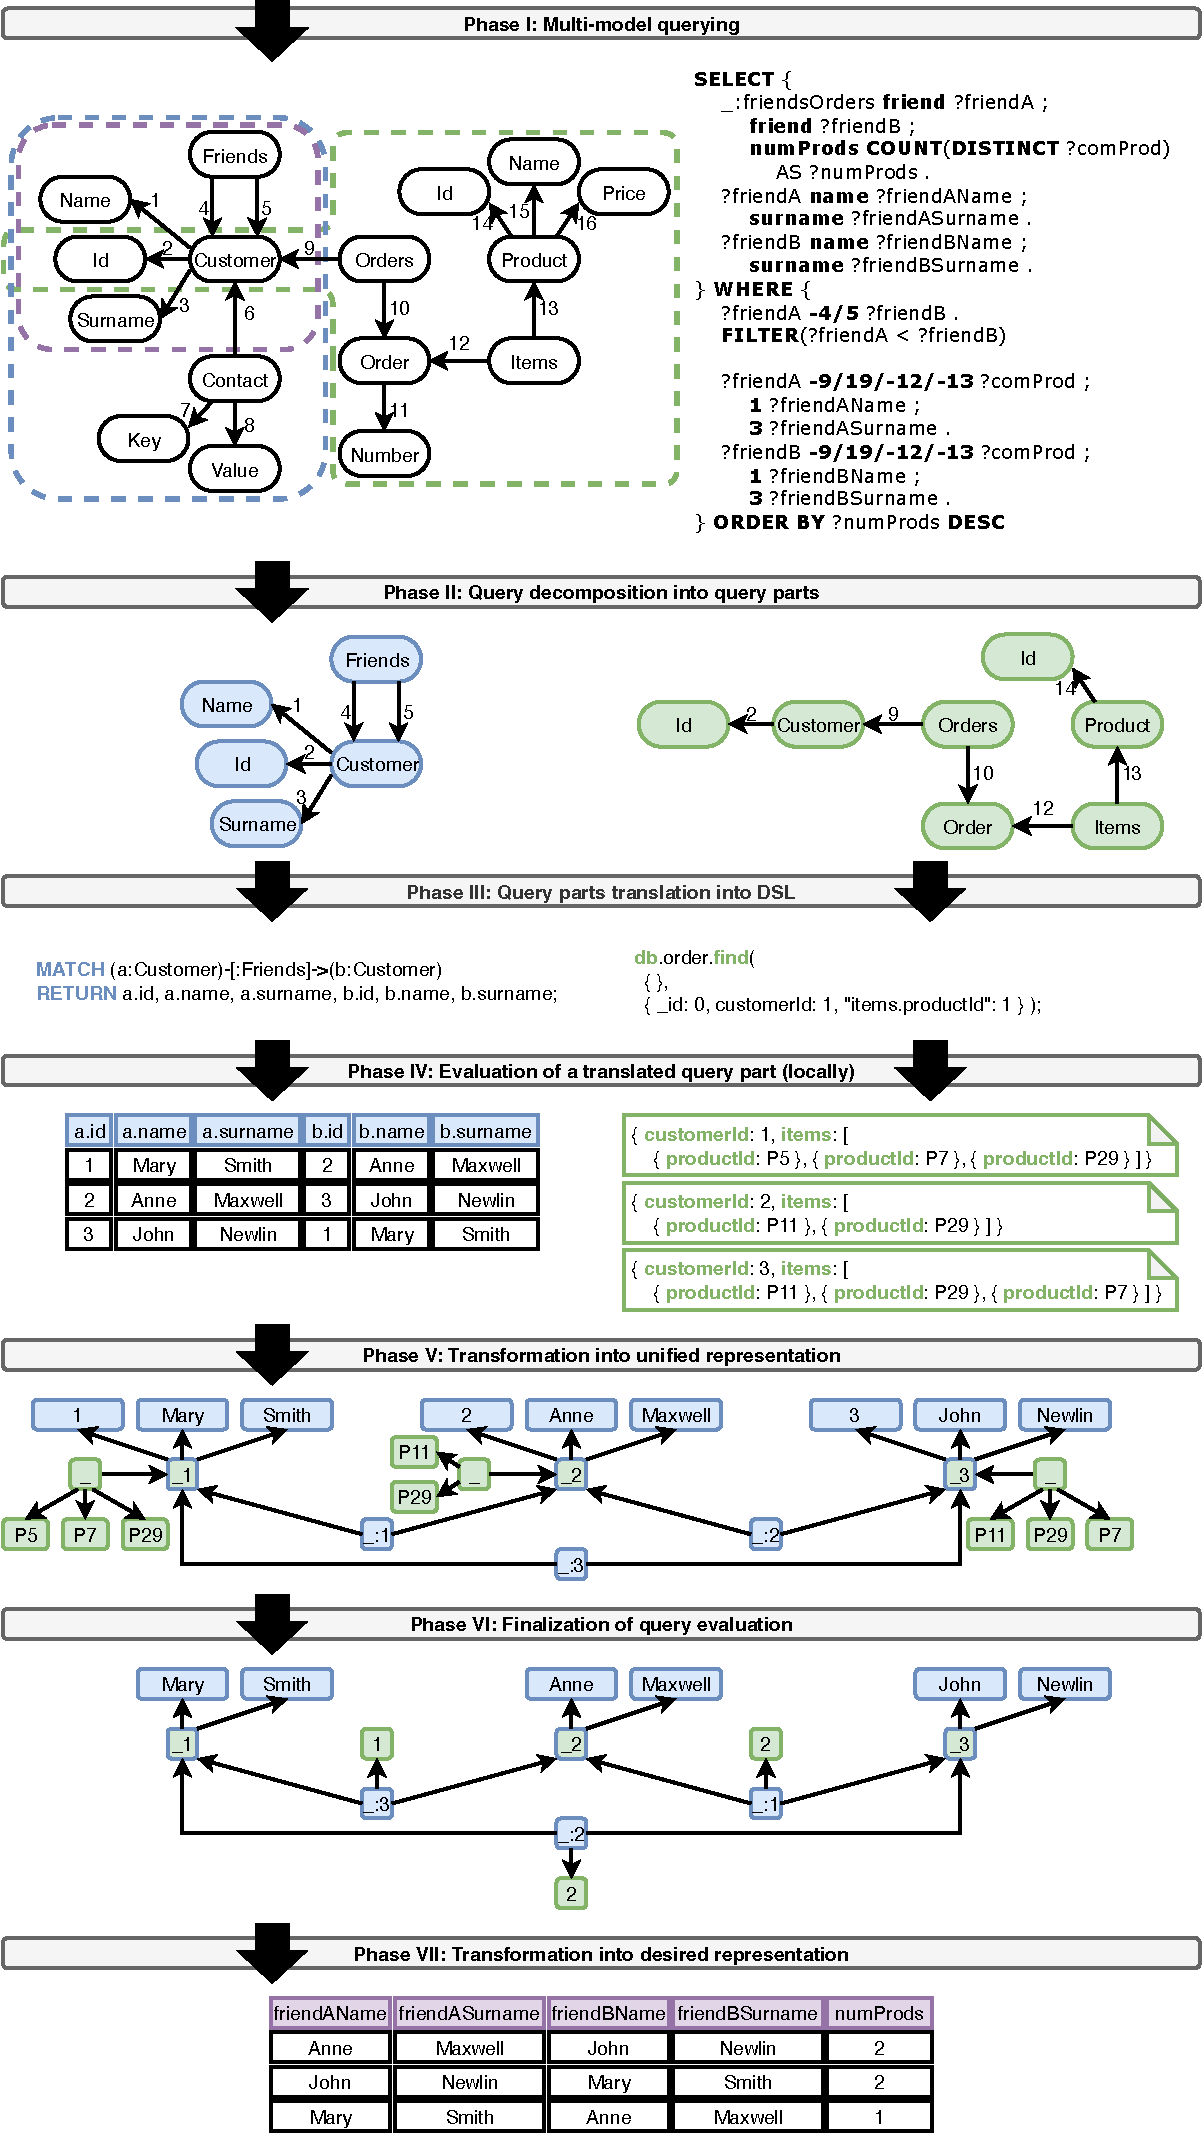
\includegraphics[width=0.9\textwidth]{img/query-workflow.pdf} 
\caption{A diagram showing the full querying workflow~\cite{mm_quecat}.}
\label{fig:queryworkflow}
\end{figure}

\subsection{Database Wrappers}
\label{algorithms:subsection:wrappers}

As we divide the MMQL query into separate query parts, the idea is for each query part to be a self-contained unit of execution which compiles down to a single native database query, regardless of the specific database.
We also wish to design our algorithms to be \textit{database agnostic}, as the spectrum of multi-model databases is vast, and we do not want to confine ourselves to a specific set of them.
Both of these facts motivate the concept of \textit{database wrappers}, which encapsulate the specifics of each database and its native query language behind a generic interface.
As the general idea of the wrappers is encapsulation of database-specific logic, we have two main requirements for the design of this generic interface:

\begin{itemize}
    \item The interface should be general enough to allow the addition of any database system which we may reasonably expect to support;
    \item The interface should abstract away all categorical concepts from the wrappers' implementations where possible to make supporting new databases easier; and
    \item The order in which wrapper interface methods are called should be irrelevant.
\end{itemize}

Perhaps the last goal is worth elaborating on -- since MMQL allows the definition of statements in any order, it is also desirable for our query translation algorithm to be able to process these statements in any order.
For this reason, all methods in the wrapper interface will make the wrapper simply "remember" this operation, and finally, when the entire query is processed, a finalization method will be called on the wrapper, building the native query.
In this way, the database wrappers operate similarly to a builder object in the builder design pattern~\cite{gof}.
With these goals in mind, we propose the following methods for the generic database wrapper interface:

\begin{itemize}
    \item \texttt{defineKind($kindId$, $kindName$)} which is an initialization function, assigning the identifier $kindId$ to the kind name $kindName$. The kind name refers to for example table names in PostgreSQL or collection names in MongoDB. Note that a single kind name can be registered multiple times under different identifiers, in which case its data is retrieved independently multiple times.
    \item \texttt{addProjection($propertyPath$, $kindId$, $variableId$)} which adds projection of a specific property to a query, i.e. given a specific kind, this method will add the specified property of this kind to the native query output.
    \item \texttt{addFilter($variableId$, $filterOp$, $constant$)} which constrains the value of a property identified by $variableId$ to a logical relation specified by $filterOp$ (such as equality or inequality), using $constant$ as the second operand. Note that the variable $variableId$ does not need to exist before this method is called, as the validation is delayed until the moment of generation of the native query. In addition, we also consider an overload \texttt{addFilter($propertyPath$, $kindId$, $filterOp$, $constant$)} which does not require its filtered property to be a part of the projection, instead specifying the path directly. This overload is necessary because of triples which contain constant literals.
    \item \texttt{addFilter($variableId_1$, $filterOp$, $variableId_2$)} which creates a relationship between the values of two variables, eliminating solutions where this relationship is not satisfied. This can be used together with aggregations, whose results have their own variable identifiers.
    \item \texttt{addValueSet($variableId$, $constants$)} which constrains the value of a property identified by $variableId$ to the set of values provided in $constants$.
    \item \texttt{addJoin($kindId_1$, $kindId_2$, $joinProperties$)} which performs a join operation on the two kinds provided. Note that we call it a join operation, but for example, in the case of the graph model, this entails a graph traversal rather than a join in the relational sense.
    \item \texttt{addRecursiveJoin($recursiveJoinPath$)} which performs a series of recursive joins between various kinds in the query part (if recursion is supported). If we have a morphism with repetition, its domain must necessarily be the same as its codomain, otherwise it would not be possible to repeat it. This kind of recursive joining is useful in cases of transitive relationship traversal (for example finding all superiors of a given company employee), and it is generally supported in the relational model with recursive common table expressions\footnote{\url{https://www.postgresql.org/docs/current/queries-with.html}}, and in the graph model with variable length paths\footnote{\url{https://neo4j.com/docs/cypher-manual/current/syntax/patterns/\#cypher-pattern-varlength}}.
    \item \texttt{addAggregation($aggregationType$, $aggregationRootKindId$,\\$rootIdPaths$, $kindId$, $propertyPath$, $variableId$)} which performs an aggregation of the specified type on the specified property of the specified kind. The aggregation may have multiple possible roots (for example averaging the item price for a set of customers, each of whom has made multiple orders with multiple items - should we average the items per order, or per customer?), and for this reason, the aggregation root is also specified, along with one of its identifiers. The result of this aggregation is stored in the variable identified by $variableId$.
    \item \texttt{buildQuery()} which takes the information collected from all method calls on this wrapper and generates the native database query based on it. This method contains the majority of the actual wrapper logic, with the other methods mostly just storing the arguments for processing by this method. The result of this method is a tuple ($nativeQuery$, $variableMap$), where $nativeQuery$ is the built native query in a string representation, and $variableMap$ contains a map of variable identifiers included in the projection to property paths within the native query result.
\end{itemize}

Naturally, not all databases support all of these operations, for example Cassandra does not support joins\footnote{We only consider the built-in capabilities of the given databases, not user-defined procedures.}.
For this reason, each database wrapper also exposes the following properties about the functionality the underlying database has:

\begin{itemize}
    \item \texttt{isJoinSupported} which specifies whether the database supports (inner) joins. For example, most relational databases do, as do graph databases in the form of graph traversals. Document databases may support joins, but for example MongoDB only supports left outer joins. Naturally, the inner join operation can be emulated using the left join operation, but the wrapper implementer may not want to support this due to the involved complexity. Finally, some databases like Cassandra do not support joins of any kind.
    \item \texttt{isOptionalJoinSupported} which specifies whether the database supports optional (left outer) joins. This is necessary because of the \texttt{OPTIONAL} clause in MMQL. In the situation that optional joins are not supported, the joins must be performed at the categorical level.
    \item \texttt{isNonIdFilterSupported} which specifies whether the database supports filtering of properties outside of the identifier set of the root object of a given kind. For example, many key-value databases treat stored values as opaque objects, not allowing filtering based on their value, but only their retrieval.
    \item \texttt{isCountAggregationSupported} which specifies whether the database supports the \texttt{COUNT} aggregation. We also define a corresponding property for each type of aggregation supported in MMQL.
    \item \texttt{isRecursionSupported} which specifies whether the database supports recursive queries, which may necessitate the recursive joining of kinds. Such joins are generally supported in relational and graph databases, and allow the traversal of tree or graph structures in a single query.
\end{itemize}

For each interface method mentioned, we will also define an optional counterpart which means that this operation should be included in the query, but with optional semantics.
In some cases, the implementations will be identical (for example in SQL, adding projection on an optional column will return \texttt{NULL} if that column is not set for a particular row).
However, in some cases, there may be differences (for example in SQL, we would generate an inner join for a non-optional join operation, whereas we would generate a left outer join in the optional case).
When defining the interface methods, we used a set of arguments which must also be explained in detail:

\begin{itemize}
    \item $propertyPath$ is an ordered list of property names, forming a traversal from the kind root to a leaf property. This property path, along with name information (for example, whether the name is dynamic), also carries the property type at each level, in order to allow database wrappers to correctly deal with nested objects and arrays. The argument $rootIdPaths$ is a list of property paths.
    \item $kindId$ is the identifier of the kind to which this operation applies. This identifier can be mapped to the kind name configured in the database wrapper at initialization time. The inclusion of an identifier instead of a name allows us to query the same kind multiple times within a query part, for example joining customers together with other customers based on the equality of their names. Similarly, $kindName$ refers to the name of the kind identified by $kindId$ in its respective database.
    \item $variableId$ identifies the output field of the native query. We cannot generally make assumptions about how the query output may be structured, as this decision is ultimately up to the database wrapper. For this reason, whenever defining a property which should be part of the native query output, we assign it a variable identifier. When the native query is compiled, the database wrapper returns a mapping of variable identifiers to concrete property paths within the query output, allowing us to parse this output into a categorical representation correctly.
    \item $joinProperties$ contains a set of tuples, with each tuple containing a property path within the corresponding kind. These tuples define join points for the join operation. Note that a limitation of our approach is that we only support joins on \textit{equality}. In theory though, joins with more complicated conditions could also be supported. 
    \item $aggregationType$ specifies the type of aggregation which should be performed, like counting or averaging.
    \item $recursiveJoinPath$ is a list of join path segments, where each join path segment may either be a tuple ($kindId_1$, $kindId_2$, $joinProperties$) symbolizing a join between two kinds, a path segment with a repetition specifier ($?$, $*$ or $+$ as in regular expressions), or multiple path segments chained together. In this way, we can represent arbitrary morphism paths with repetitions as sequences of joins between kinds, with some subsequences optionally repeated as necessary. Note that whenever a path segment is repeated, its first kind must be the same as its last kind in order for the repetition to be valid.
\end{itemize}

With the database wrapper interface specified, we can see that in its simplest form, implementing a database wrapper is actually rather straightforward.
In order to support a new database in the most minimal form possible, we can simply implement the function \texttt{addProjection}, at which point we will be able to query any data from this database, even though we would not be able to filter this data or perform joins and aggregations at the database level, forcing them to be executed in a slower way at the instance category level.

\section{Algorithms}

In~\cref{algorithms:section:approach}, we described the high-level steps involved in our proposed approach for the implementation of MMQL.
In this section, we will examine the outlined steps in greater detail, specifying a concrete algorithm for each, as well as discussing the presented algorithms and their weaknesses.

Before we start discussing the particulars of the individual algorithms, we need to discuss one key characteristic of our proposed approach.
As we attempted to divide the whole approach into a number of well-defined, easily digestible algorithms, we were faced with a decision.
On one hand, we could try to propose an algorithm which attempts to translate the query as a whole into native database queries, taking into account all parts of the MMQL query such as projection and ordering.
However, as we discovered during the design process, such an approach would result in a monolithic, very complex algorithm which is hard to reason about, making its modifications or analysis impractical.
For this reason, we opted for a simplification in this matter -- when creating a query plan and dividing the query into query parts, we only consider the contents of the query's \texttt{WHERE} clause, as this clause is actually the only truly necessary part for the retrieval of data from databases.
In this way, we are able to limit the query part translation algorithm to a set of graph patterns and a few other concepts.
This has some implications for the possible performance of our approach, as all query elements outside the scope of the \texttt{WHERE} clause must be handled by the MMQL query engine, which is undoubtedly much less efficient than using native database queries where possible.
However, as a whole, this allowed us to greatly simplify and modularize the proposed algorithms.

In general, we will discuss performance optimization possibilities when presenting the algorithms, but we will not include these optimizations in the algorithms themselves for the sake of simplicity.

\subsection{Query Preprocessing}
\label{algorithms:subsection:preprocessing}

As mentioned in the introduction to this chapter, when constructing native database queries, we will only consider the \texttt{WHERE} clause of the MMQL query.
However, before we proceed with the main parts of the querying process, we need to perform a couple of additional steps first.
One thing which needs to be done is general adjustments to the query structure to make its processing easier in the following steps.
However, as the \texttt{WHERE} clause has the semantics of inducing a schema category, we will also need to construct this schema category for further usage.
In addition to constructing this schema category, we will also need to construct the corresponding mappings.
Lastly, query validation should be a part of this process, like the validation of variable types.
We will not present any validation algorithms as they would be relatively straightforward, and for the rest of this chapter, we will assume that input queries are well formed and valid.
The full query preprocessing algorithm is shown in~\cref{algo:alg:preprocessing}, and we will shortly discuss its constituent parts in greater detail.

\subsubsection{Query Modifications}

In~\cref{mmql} during the introduction of MMQL, we mentioned its power in the form of graph patterns, including constructs like ending triples with a semicolon instead of a period to repeat the same subject in multiple triples.
However, as these constructs are simply syntactic sugar, we convert them to sets of triples with an explicitly specified subject to simplify their further processing (lines 1-9 in \cref{algo:alg:preprocessing}).

\begin{algorithm}
\small
\DontPrintSemicolon
\SetKwProg{Fn}{function}{:}{}
\SetKw{return}{return}

\KwIn{$\mathbf{SELECT}$  -- query SELECT clause\;} 
\myinput{$\mathbf{WHERE}$ -- query WHERE clause\;}

\ForEach{\textup{graph pattern $P$ in $SELECT \cup WHERE$}}{
    \If{\textup{$P$ has repeated subject $subject$ and morphism $morphism$}}{
        delete $P$ from query

        \ForEach{\textup{$object$ in $P$}}{
            add triple $subject$ $morphism$ $object$ to query
        }
    }
    \ElseIf{\textup{$P$ has repeated subject $subject$}}{
        delete $P$ from query
        
        \ForEach{\textup{$morphism$, $object$ in $P$}}{
            add triple $subject$ $morphism$ $object$ to query
        }
    }
}

\ForEach{\textup{triple $subject$, $morphism$, $object$ in $WHERE$}}{
    \If{\textup{$morphism$ is compound and not repeated}}{
        $b$ := getBaseMorphisms($morphism$)
        
        delete triple $subject$ $morphism$ $object$ from $WHERE$

        $prevVar$ := $subject$
        
        \ForEach{\textup{$baseMorphism$ in $b$}}{
            \If{\textup{$baseMorphism$ is the last element in $b$}}{
                $newVar$ := $object$
            }
            \Else{
                $newVar$ := getUniqueVarName()
            }
            
            add triple $prevVar$ $baseMorphism$ $newVar$ to $WHERE$
        }
    }
}

\ForEach{\textup{triple $subject$, $morphism$, $object$ in $WHERE$}}{
    \If{\textup{$morphism$ is base}}{
        \If{\textup{$morphism$ is $- oppositeMorphism$}}{
            delete triple $subject$ $morphism$ $object$

            add triple $object$ $oppositeMorphism$ $subject$
        }
    }
}

\caption{Query Preprocessing Algorithm.}
\label{algo:alg:preprocessing}
\end{algorithm}

The most interesting part of the query preprocessing step is \textit{compound morphism decomposition} (lines 10-20 in \cref{algo:alg:preprocessing}).
Recall that in MMQL, we may specify compound morphisms using the syntax \texttt{55/31}, meaning the traversal of morphism with signature \texttt{55}, followed by the traversal of morphism with signature \texttt{31}.
Again, as we attempt to make the query processing simple, we decompose all compound morphisms into base morphisms\footnote{For the purposes of the algorithms in this chapter, we will consider base morphisms to be traversals of a base morphism in any direction.}, inserting technical temporary variables with unique names in between the base morphisms.
An example of this can be seen in~\cref{algo:figure:decomposition}, where we can see a triple containing a compound morphism, and the decomposed representation of this triple.
As far as MMQL is concerned, both of these constructs are semantically equivalent.
Finally, for each morphism, we can also traverse it in the opposite direction with the MMQL unary minus operator.
Without loss of generality, we can reverse the direction of traversal for base morphisms along with swapping the subject and object, which simplifies further processing of these opposite-direction traversals (lines 21-25 in \cref{algo:alg:preprocessing}).

\begin{figure}[ht]
\begin{code}
WHERE {
    // Compound morphism before preprocessing
    ?customer 55/31 ?orderNumber .

    // Decomposed compound morphism with inserted variable
    ?customer 55 ?51d747110d95 .
    ?51d747110d95 31 ?orderNumber .
}
\end{code}
\caption{Compound morphism decomposition.}\label{algo:figure:decomposition}
\end{figure}

Note that compound morphism decomposition only applies to compound morphisms without repetition.
When morphisms with repetition are encountered, they are left intact, as it may be necessary to form recursive queries in this instance, and it is not possible to decompose morphisms with infinite upper bound repetition.

The inquisitive reader may raise the question of optimization -- is it possible for the query engine to omit "useless" data along the path of the compound morphism, only retrieving the data necessary for the query variables?
However, recall~\cref{categorical:chapter} where we introduced the notion of the schema and instance category.
The instance category must conform to its corresponding schema category, meaning that if our schema category has base morphisms \texttt{55} and \texttt{31}, these morphisms must also exist as instance morphisms, making this kind of optimization impossible if we intend to stick with the categorical model throughout the process.
Not all hope is lost though, as there is a way to make this optimization work.
If the query engine notices that a particular set of morphisms is only ever traversed together in a compound morphism, it could perform a contraction of these morphisms in the schema category, defining a new schema category where this compound morphism is transformed into a single base morphism.
In this fashion, the instance category would now contain the formerly compound morphism as a base morphism, allowing the query engine to omit irrelevant data from the query plan.

\subsubsection{Constructing the Schema Category}

As we mentioned in the introduction of this subsection, before we may continue with the rest of the process, we must first construct the schema category induced by the \texttt{WHERE} clause, which will be used in the following subsections.
The original schema category which the query was made with is therefore only used as the input for the algorithm for the construction of the schema category induced by the \texttt{WHERE} clause, which we will introduce shortly.
The same applies to the original mappings, which must also be adjusted.
However, before we explain \textit{how} this is done, we should mention \textit{why} it needs to be done.
In fact, if we have a query which contains a maximum of one variable per schema object, this step is totally unnecessary.
The reason for the existence of this step is queries which have multiple variables corresponding to the same schema object (for example, recall~\cref{mmql:figure:samevar}, showing a query selecting two different customers who purchased an item with the same name).
In this case, we need a way to separate the values of both variables, as their possible sets of values may not be the same.

To solve the issue of multiple variables per schema object, we propose a modification to the original schema category.
We will not provide an explicit algorithm for this, as its creation from the following definitions is straightforward.
Let $\mathbf{S}$ = $(\mathcal{O}_\mathbf{S}, \mathcal{M}_\mathbf{S}, \circ_\mathbf{S})$ be the original schema category (recall~\cref{categorical:section:schema}), and let $\mathbf{Var}_{WHERE}$ be the set of variables in the query \texttt{WHERE} clause.
We will define $\mathbf{S}_{WHERE}$ := $(\mathcal{O}_{\mathbf{S}_W}, \mathcal{M}_{\mathbf{S}_W}, \circ_{\mathbf{S}_W})$
For each $var \in \mathbf{Var}_{WHERE}$ and $o \in \mathcal{O}_\mathbf{S}$, we define a schema object $o_{var} \in \mathcal{O}_{\mathbf{S}_W}$ whose instances will contain the values of variable $var$.
Additionally, as the query does not need to contain all (or any) identifiers of any particular schema object which is part of the query, we also add all schema objects necessary for all identifiers of all objects $o_{var} \in \mathcal{O}_{\mathbf{S}_W}$ to $\mathcal{O}_{\mathbf{S}_W}$.
These additional objects are inserted separately for each $o_{var} \in \mathcal{O}_{\mathbf{S}_W}$, they are not shared in the case that multiple variables refer to the same schema object in $\mathbf{S}$.

For each $o_{var1}, o'_{var2} \in \mathcal{O}_{\mathbf{S}_W}$ and $m = (s, o, o', min, max) \in \mathcal{M}_\mathbf{S}$, if the triple \texttt{?var1 s ?var2} exists in the \texttt{WHERE} clause, then we define\\ $m_{var12} := (s_{var12}, o_{var12}, o'_{var12}, min, max) \in \mathcal{M}_{\mathbf{S}_W}$.
In addition, just as we did with schema objects, we will define the required morphisms to satisfy all identifiers of all $o_{var} \in \mathcal{O}_{\mathbf{S}_W}$ to be part of $\mathcal{M}_{\mathbf{S}_W}$.
Using these definitions, we will also consider morphism signatures $s$ to be equivalent to $s_{var12}$ when used in triples of the form \texttt{?var1 s ?var2} in the rest of this chapter when working with $\mathbf{S}_{WHERE}$.
This allows us to reason more simply about the query processing algorithms, as we can keep using signatures specified in the query to refer to corresponding signatures from $\mathbf{S}_{WHERE}$, since given a triple, this mapping is always unambiguous.

Finally, we define $\circ_{\mathbf{S}_W}$ to be the natural extension of $\circ_\mathbf{S}$ over $\mathcal{M}_{\mathbf{S}_W}$.
We show an example of the construction of this induced schema category using a schema category shown in \cref{algo:fig:induced_cat_original} and a query shown in \cref{algo:fig:induced_query}, with the schema category induced by the query's \texttt{WHERE} clause being shown in \cref{algo:fig:induced_cat_new}.
Note that the \texttt{Surname} schema object is missing, as it is not part of the query's \texttt{WHERE} clause, nor is it part of any object's $ids$.

\begin{figure}
\centering
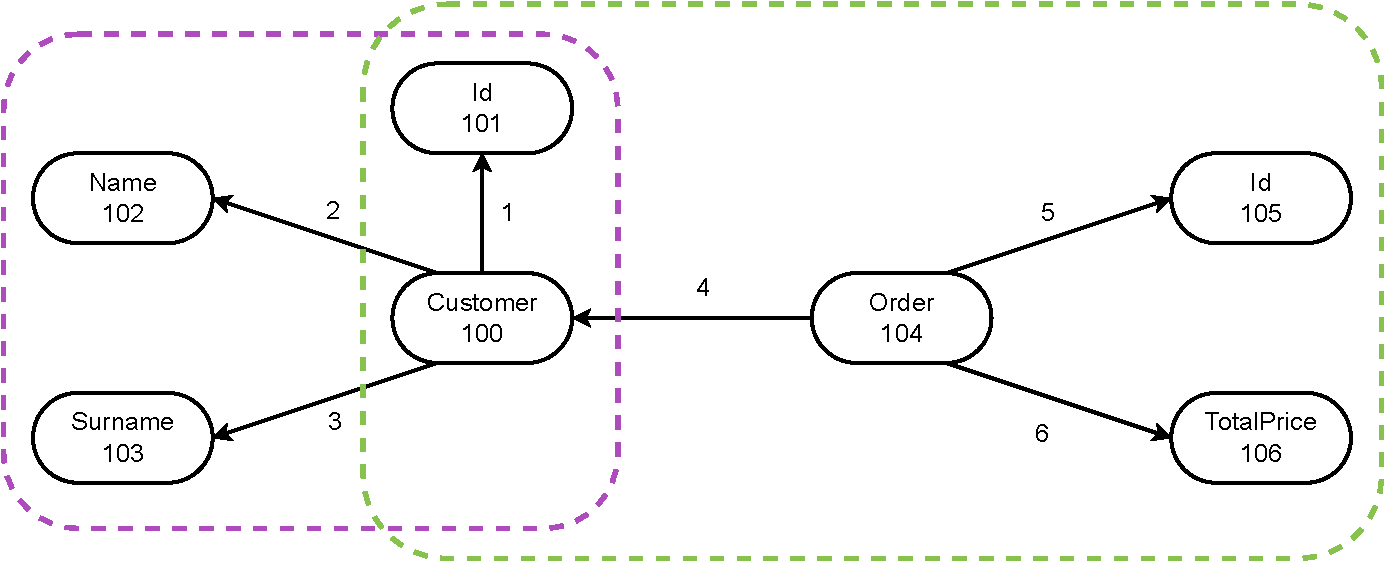
\includegraphics[width=\textwidth]{img/induced-category-original.pdf} 
\caption{A sample schema category showing a set of customers in a relational database, and a set of orders in a document database, with each order containing the identifier of the ordering customer.}
\label{algo:fig:induced_cat_original}
\end{figure}

\begin{figure}
\begin{code}
SELECT {
    _:shared name ?sharedName ;
        price ?sharedPrice .
}
WHERE {
    ?customer1 2 ?sharedName ;
        -4 ?order1 .

    ?customer2 2 ?sharedName ;
        -4 ?order2.

    ?order1 6 ?sharedPrice .
    ?order2 6 ?sharedPrice .
}
\end{code}
\caption{A query returning two customers with the same name who placed an order with the same total price, corresponding to the schema category shown in \cref{algo:fig:induced_cat_original}.}\label{algo:fig:induced_query}
\end{figure}

\begin{figure}
\centering
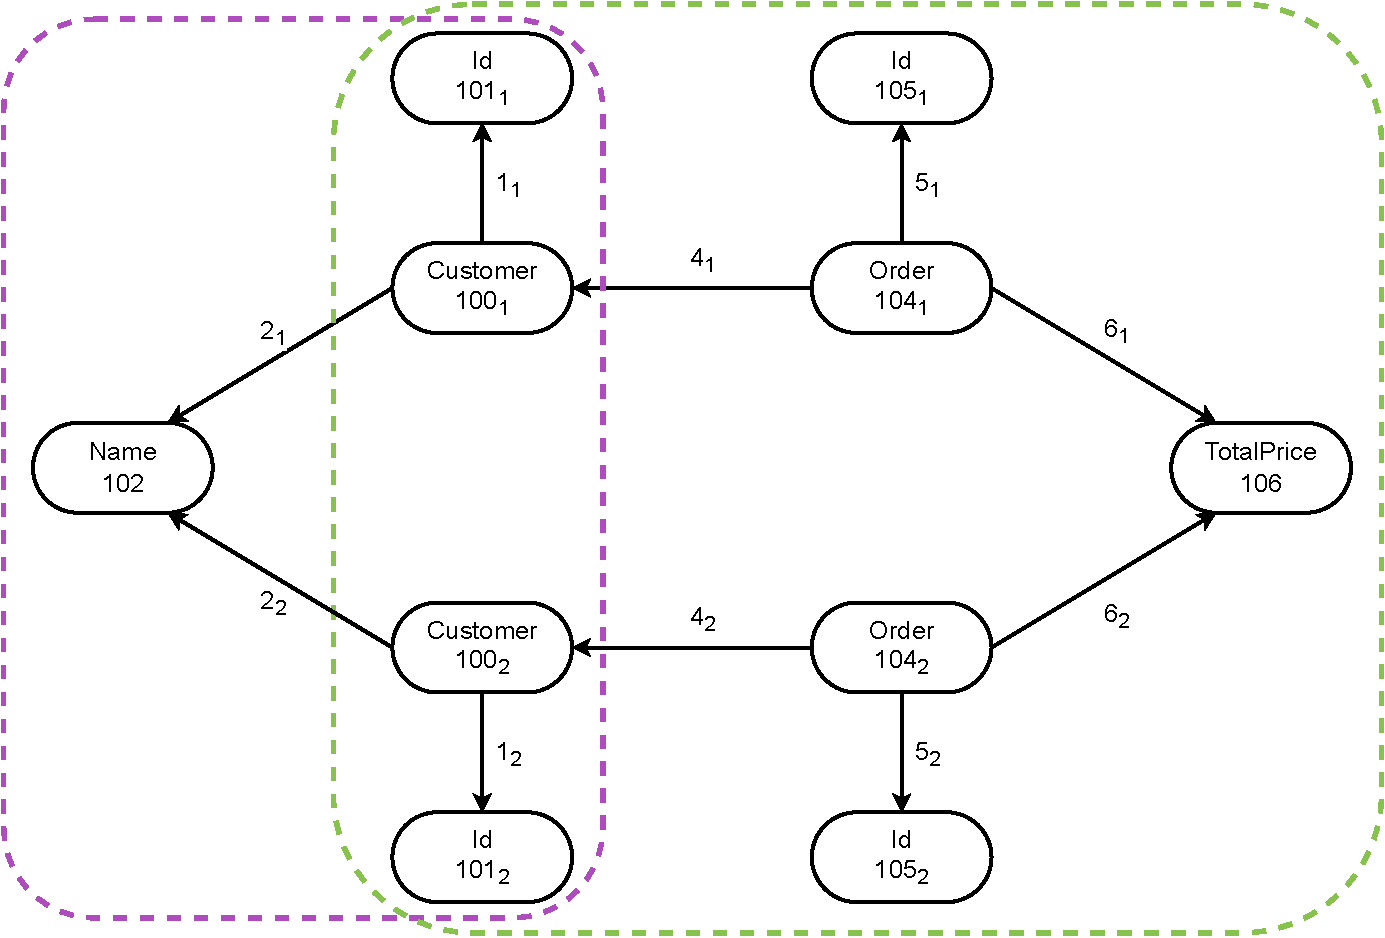
\includegraphics[width=\textwidth]{img/induced-category-new.pdf} 
\caption{Schema category induced by the WHERE clause of the query shown in \cref{algo:fig:induced_query}.}
\label{algo:fig:induced_cat_new}
\end{figure}

We need to mention that the \texttt{WHERE} clause may contain the \texttt{OPTIONAL}, \texttt{UNION} and \texttt{MINUS} clauses in addition to graph patterns and filters.
As far as the generation of the new schema category goes, \texttt{OPTIONAL} is quite simple, as we simply consider its contents the same way as non-optional graph patterns, save for modifying the morphism cardinality at join points to have a minimum of zero, as the optional parts may or may not exist.
It is remarkably similar for \texttt{MINUS}, where we can treat the forbidden pattern as an optional pattern, using it to filter the final result set.
In the case of \texttt{UNION}, we simply consider both of its operands to be optional as far as the schema category is concerned.

As for nested queries, they are evaluated recursively from the most nested to the least nested, and their results are joined to the containing query's \texttt{WHERE} clause.
This means that at the level of the schema category, we simply need to define the appropriate schema objects corresponding to the results of the nested query.

\subsubsection{Constructing New Mappings}

With the new schema category $\mathbf{S}_{WHERE}$ in hand, we naturally also need to adjust the set of mappings $\mathfrak{M}$ corresponding to $\mathbf{S}$ to be valid for $\mathbf{S}_{WHERE}$.
This is necessary because these modified mappings $\mathfrak{M}_{WHERE}$ will be used for the generation of query plans and the translation of query parts to native database queries, both of which operate on the $\mathbf{S}_{WHERE}$ schema category.
Before continuing, it is recommended that the reader is intimately familiar with the concepts introduced in~\cref{categorical:section:mapping}.
It is also worth remembering that for queries with at most one variable per schema object, this operation is effectively a no-op, and its purpose is to correctly handle queries with multiple variables per one schema object.

As we mentioned earlier, we restrict our approach to queries for which every property selection from a kind must necessarily contain the entire property path from the root.
For this reason, it is sufficient to examine only kinds whose root objects are present in the query.

Given $\mathfrak{M}$, let us define $\mathfrak{M}_{WHERE}$ in the following way.
For each mapping $\mathfrak{m} \in \mathfrak{M}$ with root object $o$, discard it if its root object is not part of the query.
Otherwise, for each $o_{var} \in \mathcal{O}_{\mathbf{S}_W}$, we define $\mathfrak{m}_{var} \in \mathfrak{M}_{WHERE}$.
For each property $\phi \in \mathfrak{m}$, we define the corresponding property $\phi' \in \mathfrak{m}_{var}$ recursively by replacing occurrences of signatures $s \in \mathbf{S}$ with signatures $s_{varxy} \in \mathbf{S}_{WHERE}$ for the corresponding objects $o_{varx}, o_{vary} \in \mathbf{S}_{WHERE}$.
This formulation seems complicated, but when explained with plain words, it is actually rather straightforward -- for each schema object in $\mathbf{S}_{WHERE}$ which is the root of some kind's mapping, we are simply constructing an equivalent mapping, but using the new variable-specific objects and morphisms from $\mathbf{S}_{WHERE}$.
For example, let us consider a query selecting two different customers, with the customer kind having its own mapping.
This definition would create two instances of this mapping, each for one of the customer variables, in such a way that when querying the customers' data from the database, the correct data ends up in the correct customers' instance objects, taking into account that some may be shared due to the shape of the query.
We can see an example of such mappings in \cref{algo:fig:induced_cat_mappings}, which correspond to the schema category shown in \cref{algo:fig:induced_cat_new}.

\begin{figure}[ht]
\centering
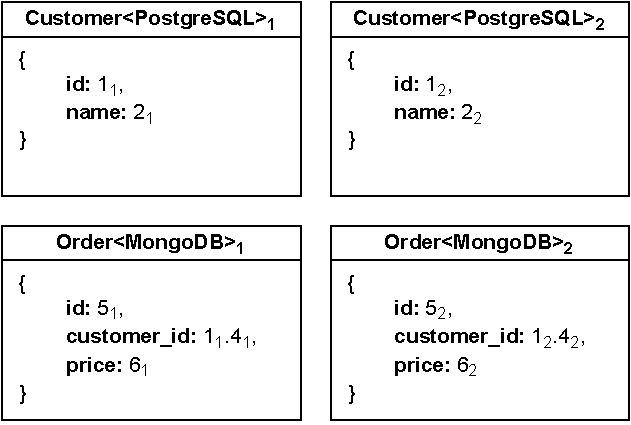
\includegraphics[width=0.75\textwidth]{img/induced-category-mappings.pdf} 
\caption{Mappings corresponding to the induced schema category shown in \cref{algo:fig:induced_cat_new}.}
\label{algo:fig:induced_cat_mappings}
\end{figure}

Note that it may be necessary for a single property $\phi$ to produce multiple properties $\phi'$, $\phi''$ and so on.
This can happen in the specific cases of nested arrays in the mapping, as we are able to bind multiple distinct variables to different elements of the array.
We do not need to give this scenario any special consideration, as long as we presume that given $\phi'$ or $\phi''$, we are able to determine $\phi$, allowing us to correctly construct the appropriate database query during the translation of query parts.

\subsection{Query Plan}
\label{algo:subsection:queryplan}

Now that the query has been preprocessed, the query engine must first create a set of query plans dictating how the query will be executed (recall Phase II in \cref{fig:queryworkflow}).
In simple terms, we consider a query plan to be a plan of which data will be retrieved from which database, and in what way.
When we consider the situation of no data redundancy, we only need to consider a single query plan on the level of MMQL, as there is only one database from which we can retrieve any given kind.
Naturally, the databases' query planners will come into play under the covers, and during the execution of native database queries, the database planners will certainly consider a number of different plans.
However, in the context of MMQL, the query planner only needs to decide where to retrieve the data from, and the optimization of native queries is left up to the databases themselves.
When we consider data redundancy, there will be multiple query plans generated on the MMQL side.

More formally, we consider a query plan to be a set of query parts, such that each distinct base morphism which is part of the MMQL query \texttt{WHERE} clause, is assigned to exactly one query part.
A query part is a set of mappings, assigning base morphisms to kinds defined in mappings.
This means that for each morphism in the query, we make a decision on which kind this morphism should be retrieved from.
The algorithm for the creation of query plans is shown in~\cref{algo:alg:queryplan}.
In simple terms, for each base morphism in the query, it retrieves the set of kinds of which this morphism is a part (lines 1-7), and then generates a set of query plans by Cartesian product of all morphism-kind assignments (lines 8-12).

\begin{algorithm}
\small
\DontPrintSemicolon
\SetKwProg{Fn}{function}{:}{}
\SetKw{return}{return}

\KwIn{$\mathbf{WHERE}$  -- query WHERE clause\;} 
\myinput{$\mathfrak{M}_{WHERE}$  -- set of mappings adjusted for the schema category induced by the WHERE clause\;}

\tcp{Map listing the set of possible source kinds for each morphism}
$morphismKindMap$ := \{\}

$queryPlans$ := [ ]

\ForEach{\textup{triple $subject$ $morphism$ $object$}}{
    \ForEach{\textup{mapping $\mathfrak{m}$ in $\mathfrak{M}_{WHERE}$}}{
        $namePath$ := getPropertyPath($morphism$, $\mathfrak{m}$)

        \If{\textup{$namePath$ is not NULL}}{
            $morphismKindMap$.append($morphism$, $\mathfrak{m}$)
        }
    }
}

$kindAssignments$ := cartesianProduct($morphismKindMap$)

\ForEach{\textup{$kindAssignment$ in $kindAssignments$}}{
    $queryPlan$ := createQueryPlan($kindAssignments$)

    \If{\textup{$queryPlan$ is not NULL}}{
        $queryPlans$.append($queryPlan$)
    }
}


\caption{Query Plan Generation Algorithm.}
\label{algo:alg:queryplan}
\end{algorithm}

There are a couple interesting functions being called in this algorithm which are worth mentioning.
The first of them is \texttt{getPropertyPath}, which given a morphism and a kind's mapping, returns an ordered list of properties which form a traversal from the kind root to the morphism within the kind.
If the morphism does not exist in the kind, this function returns \texttt{NULL}, which is why we can see this function being used to check whether a morphism lies in a given kind.

The next interesting function is \texttt{createQueryPlan}, which may be seen in \cref{algo:alg:createqueryplan}.
This function accepts a mapping of morphisms to their source kinds, and returns a query plan for this mapping.
This function's job is to divide the query into query parts, forming the query plan.
It also validates the query plan, as it only makes sense to assign a morphism to be selected from a kind when the entire property path to this morphism is also being selected from the same kind.
This has a very important consequence for the set of queries which our approach is able to process, as given this constraint, any MMQL query which is only operating on a subforest of a kind's access path which does not include the kind root object is not valid.
For example, given the schema category and access path shown in~\cref{fig:mappings}, a query only selecting order items and their names, but not containing any variable for the \texttt{Order} schema object, would produce zero valid query plans as proposed.
This is fixable by adding special cases for such queries to the algorithm, which might insert the necessary variables for a valid query plan to be generated.
However, we omitted these special cases for the sake of simplicity.

\begin{algorithm}
\small
\DontPrintSemicolon
\SetKwProg{Fn}{function}{:}{}
\SetKw{return}{return}
\SetKw{continue}{continue}

\Fn{\textup{createQueryPlan($kindAssignments$)}}{
\KwIn{$kindAssignments$ -- the source kind for each morphism\;}
    \ForEach{\textup{$morphism$, $kind$ in $kindAssignment$}}{
        $namePath$ := getNamePath($morphism$, $kind$)
        
        $isPlanValid$ := isPathInKind($kindAssignment$, $kind$)

        \If{\textup{NOT $isPlanValid$}}{
            \return{\textup{NULL}}
        }
    }

    $queryParts$ := getQueryParts($kindAssignments$)

    \tcp{A query plan is a list of query parts}
    \return{$queryParts$}
}


\caption{Function \texttt{createQueryPlan} from~\cref{algo:alg:queryplan}.}
\label{algo:alg:createqueryplan}
\end{algorithm}

Additionally, we have the \texttt{getQueryParts} function, which performs the actual division of the query into query parts.
We consider a query part to be a maximal connected component of kinds from the same database in the query in the case that the database's wrapper supports joins, or a single kind in the case that joins are not supported.
The reason for this is that we need each query part to be convertible to a single native database query, and if joins are not supported at the database level (like in Cassandra, a columnar database), each kind must be separated into its own query part.
This function is shown in~\cref{algo:alg:getqueryparts}.
There we can see a few more functions worth explaining being used, specifically \texttt{getConnectedComponents} which returns kinds contained within a given query part grouped by reachability, i.e. if there are multiple kinds within this query part which are not directly connected.
This can happen if we are selecting multiple kinds from the same database, but in between them is a kind from a different database.
There is also the \texttt{getDBWrapper} function, which returns a database wrapper for a given query part, as described in~\cref{algorithms:subsection:wrappers}.

\begin{algorithm}[ht]
\small
\DontPrintSemicolon
\SetKwProg{Fn}{function}{:}{}
\SetKw{return}{return}
\SetKw{continue}{continue}

\Fn{\textup{getQueryParts($kindAssignments$)}}{
\KwIn{$kindAssignments$ -- the source kind for each morphism\;}
    \tcp{Initial query parts are kinds grouped by their database}
    $queryParts$ := groupBy($kindAssignments$, $x$ $=>$ $x$.database)

    \tcp{If the kinds for a given query part do not form a single connected component, split this query part such that each new query part forms a connected component}
    \ForEach{\textup{$queryPart$ in $queryParts$}}{
        $disjointKindSets$ := getConnectedComponents($queryPart$)

        $queryParts$.remove($queryPart$)

        $queryParts$.extend($disjointKindSets$)
    }

    \tcp{If the database for this query part does not support joins, separate each kind into its own query part}
    \ForEach{\textup{$queryPart$ in $queryParts$}}{
        $W$ := getDBWrapper($queryPart$)

        \If{\textup{not $W$.isJoinSupported}}{
            $queryParts$.remove($queryPart$)

            \tcp{This is a simplified way of expressing that the morphism mappings for each kind in queryPart are split into a separate query part}
            \ForEach{\textup{$kind$ in $queryPart$}}{
                $queryParts$.append($kind$)
            }
        }
    }

    \return{$queryParts$}
}

\caption{Function \texttt{getQueryParts} from~\cref{algo:alg:createqueryplan}.}
\label{algo:alg:getqueryparts}
\end{algorithm}

The perceptive reader may have noticed that the presented algorithm does not take into account morphisms with repetition, which is intentional.
When we are dealing with morphisms with repetitions, things get considerably more complex, therefore they were omitted from the algorithms for the sake of simplicity.
Repeated morphisms may require special support on the database level, which is why the database wrappers contain the \texttt{isRecursionSupported} property, telling us whether we can form recursive queries in this database.
For example, this is possible in most graph databases with their path matching capabilities.
If recursion is not supported on a database level or the repeated morphism is a compound morphism crossing database boundaries, the MMQL query engine would have no choice but to emulate this functionality by itself, and perform the required joins at the level of the instance category.
This is not only extremely inefficient, but also needlessly complicated, which is why we do not present a full algorithm for this scenario.

Another thing missing from the presented algorithm is handling of \texttt{OPTIONAL}, \texttt{UNION} and \texttt{MINUS} clauses, which is intentional.
When constructing a query plan, we consider optional graph patterns as if they were not optional, assigning source kinds to morphisms.
Similarly, both \texttt{UNION} operands are considered to be optional by the query planner, as either one of them may or may not exist in any given instance.
Finally, the second operand of \texttt{MINUS} clauses is treated as if it was optional, attempting to match the pattern in the data, and removing the matching solutions.

As an example, recall the query from \cref{algo:fig:induced_query}, whose \texttt{WHERE} clause induced the schema category presented in \cref{algo:fig:induced_cat_new}.
We can see the division of the triples from this query's \texttt{WHERE} clause into query parts in \cref{algo:fig:induced_parts}.
Note that because PostgreSQL supports inner joins, both customers' data can be queried together in a single query part, but because MongoDB does not support inner joins natively\footnote{MongoDB does support the left join operation, which makes it possible to implement an inner join as well, but for the purposes of this example, we consider MongoDB as not supporting inner joins.}, the queries for the two orders need to be separated into two query parts.
The reader may have also noticed that there are some extra triples selecting the customers' identifiers, the addition of which we will discuss in \cref{algo:subsection:joinplan}.

\begin{figure}[ht]
\begin{code}[codes={\catcode`$=3\catcode`_=8}]
Query Part 1 (Customer<PostgreSQL>$_1$, Customer<PostgreSQL>$_2$) {
    ?customer1 $2_1$ ?sharedName .
    ?customer1 $1_1$ ?customerId1 .

    ?customer2 $2_2$ ?sharedName .
    ?customer2 $1_2$ ?customerId2 .
}
Query Part 2 (Order<MongoDB>$_1$) {
    ?order1 $4_1$ ?customer1 .
    ?customer1 $1_1$ ?customerId1 .
    ?order1 $6_1$ ?sharedPrice .
}
Query Part 3 (Order<MongoDB>$_2$) {
    ?order2 $4_2$ ?customer2 .
    ?customer2 $1_2$ ?customerId2 .
    ?order2 $6_2$ ?sharedPrice .
}
\end{code}
\caption{Decomposition of triples into query parts based on the query shown in \cref{algo:fig:induced_query}.}\label{algo:fig:induced_parts}
\end{figure}

\subsection{Join Plan}
\label{algo:subsection:joinplan}

With a set of query plans generated by the algorithm presented in the previous subsection, one may think that we are ready to select the best query plan and continue with query execution.
However, there is one more thing that needs to be done beforehand, as it may have an impact on the choice of the best query plan.
We are talking about \textit{join plans} -- since we are dealing with multi-model data, it is likely that we will have a query with multiple query parts, with the necessity of joining their results together to get the full query result.

In general, join order optimization is a known hard problem~\cite{join_order}, with multi-model join optimization is even harder with relatively little related work to fall back on, which is why attempting to solve it would be outside the scope of this thesis.
For this reason, in this subsection, we will discuss join plans in a slightly different fashion.
For our purposes, a join plan is a set of join points in the query, where each join point consists of neighboring kinds, as well as the \textit{join identifier}.
The join identifier is one of the $ids$ (recall~\cref{categorical:section:schema}) of the schema object which the given kinds need to be joined on.

In general, the properties which are a part of the $ids$ of any given schema object do not need to be a part of the query, even if the object itself is a part of it.
However, if this object happens to be the join point between two kinds, this would pose an issue, because we need one of that object's identifiers in order to determine how to join the data from both kinds.
For this reason, if none of the object's identifiers are a part of the query, we will need to insert the selection of at least one such identifier to make the join possible.
Note that there can even be multiple objects which are part of a single join point between two query parts, which is why we need to consider all of them.
Therefore, in this subsection, we present~\cref{algo:alg:joinplan}, where we show our proposed approach of finding all join points for a given query plan, and the selection of the necessary identifiers.

The join plan algorithm identifies join points by looking for specific patterns in the query plan (line 5 in \cref{algo:alg:joinplan}).
These patterns involve two neighboring query parts, having a triple from each query part, with both triples sharing a schema object.
This shared schema object which forms the intersection of the query parts must be part of both triples, but the direction of the triples is irrelevant, i.e. the intersection object may be either the subject or object of the given triples.
Once the intersection object is found, its identifiers are examined, and an identifier is selected which may be queried using both kinds at the join point.
Then, the selection of this identifier from the intersection object is added to both query parts in the form of triples with unique variable names (if not already present).

A special case to consider is when the intersection object has a signature of $\epsilon$, meaning the object is identified only by its value.
This means that we are joining two query parts by the value of an attribute, like joining two different customers on the equality of their name.
In this case, no extra work is needed, as the value necessary for the join is already being selected.

\begin{algorithm}[ht]
\small
\DontPrintSemicolon
\SetKwProg{Fn}{function}{:}{}
\SetKw{return}{return}
\SetKw{break}{break}

\KwIn{$queryPlan$  -- the query plan for which we need to create a join plan\;}

\ForEach{\textup{neighboring query parts $q1$, $q2$ in $queryPlan$}}{
    \ForEach{\textup{triple $t1$ in $q1$, triple $t2$ in $q2$}}{
        $m1$ := $t1$.morphism

        $m2$ := $t2$.morphism
        
        \tcp{The parentheses in this pattern mean schema objects, and the labeled dashes represent morphisms. We match the pattern regardless of the direction of traversal of the morphism, which is why they are depicted as undirected.}
        \If{\textup{$t1$ and $t2$ match the pattern () -$m1$- ($I$) -$m2$- ()}}{
            $ids$ := getIds($I$)

            $k1$ := getKind($t1$)

            $k2$ := getKind($t2$)

            \ForEach{\textup{$id$ in $ids$}}{
                \If{\textup{$id$ is $\epsilon$}}{
                    $queryPlan$.joinPoints.add(($q1$, $q2$, $I$, $id$))

                    \break
                }
            
                \If{\textup{$id$ can be selected from $k1$ and $k2$}}{
                    $r1$ := getRootObject($k1$)

                    $r2$ := getRootObject($k2$)
                
                    \ForEach{\textup{$prop$ in $id$}}{
                        \If{\textup{$prop$ is not selected from $I$ in $q1$}}{
                            add triples selecting $prop$ from $I$ to $q1$
                        }

                        \If{\textup{$prop$ is not selected from $I$ in $q2$}}{
                            add triples selecting $prop$ from $I$ to $q2$
                        }
                    }

                    $queryPlan$.joinPoints.add(($q1$, $q2$, $I$, $id$))

                    \break
                }
            }
        }
    }
}

\caption{Join Plan Algorithm.}
\label{algo:alg:joinplan}
\end{algorithm}

Finally, we mentioned earlier in this subsection that we do not attempt to solve the hard problem of multi-model join order optimization.
In our implementation of the core parts of these algorithms (described in~\cref{quecat}), we will mention that we are using software called MM-evocat~\cite{evocat}, which provides us with the functionality of merging instance categories together.
For this reason, we do not need to worry about coming up with a basic replacement for a join order optimizer, because if we send query parts to MM-evocat to process in parallel, MM-evocat decides the order of the joins, relieving us of the responsibility.

\subsection{Picking the Best Query Plan}
\label{algo:subsection:bestplan}

As a result of our work in the last subsection, we now have a set of query plans, each of which has an associated join plan (which does not define the order of joins, but rather the set of joins itself).
The next thing we need to do is we need to pick a query plan.
However, this turns out to be much more complicated than it sounds.
Single-model query planning and optimization are already known to be a hard problem~\cite{query_optimization}.
When we move into the world of multi-model data, polystores like BigDAWG\footnote{\url{https://bigdawg.mit.edu/}} include multi-model query planners and optimizers, but these do not fit neatly to our problem domain due to the number of extra considerations owing to our categorical data representation.
For this reason, proposing an approach for the problem of multi-model query planning and optimization is outside the scope of this thesis.
However, for the benefit of future work on this subject, we will discuss the possible inputs which could be used for the development of a suitable multi-model query planner for MMQL.

When it comes to the information we already have, the query planner could take into account various features of the query plans themselves.
For example, the number of databases used in the query may be relevant, as it is likely that a query which utilizes 4 databases to retrieve the same data as a query utilizing only 2 databases may be less performant.
The specific databases used may also be relevant, as the query planner could use information about the current load on the databases to select a plan which utilizes databases which are not overloaded.
Another piece of information for a multi-model query planner to consider is the amount of work necessary to perform additional work on the MMQL query engine side, like projection, ordering, or deferred statements which will be introduced shortly in~\cref{algo:subsection:translation}.
The cost of these tasks is prohibitively high, especially for large amounts of data, which is why they should be avoided at all costs.

In addition, a multi-model query planner working with multiple databases can rely on the single-model query planners native to those databases.
Most databases expose some kind of functionality which allows users to access information about the query planner.
For example, SQL has the \texttt{EXPLAIN} keyword, which when used together with a query, will return information like the total plan cost (generally expressed in abstract units, but sometimes also in units like the approximate number of disk accesses necessary), information about which indexes the query is using, or the approximate number of rows which may be returned by the query.
In this way, the query planner might avoid slow queries which do not have indexes available, and prefer faster queries which are able to use indexes.
Similarly, the Neo4j query planner can estimate the number of rows returned by various stages of the query.
Examples of the outputs of the PostgreSQL and Neo4j query planners can be seen in \cref{attachment:plannerpostgresql} and \cref{attachment:plannerneo4j} respectively.
Note that in order to make use of the generated native queries, the query planner would need to defer the choice of best plan one step further in the process, meaning query translation would need to happen for each generated query plan, and only then would the best plan be selected.

For some databases, the information returned by their query planner may be less useful however.
For example in MongoDB, the query planner is able to say whether a given query will use an index without actually executing the query, but does not give any kind of cost estimate.
To get the cost associated with a given query, one must execute the query using an explain command, which runs the query and only then returns the cost.
We can see examples of both modes of operation of the MongoDB query planner in \cref{attachment:explainmongodb}.
In general, a multi-model query planner should ideally take into account all of this information to make an educated guess about the cost of each query plan, selecting the plan with the lowest cost for execution.
Similarly, such a query planner should expose information about its decision making process to allow users to better understand the query plans, and potentially add indexes to the relevant databases to make queries more performant.

\subsection{Translation}
\label{algo:subsection:translation}

Now that we have constructed and selected a query plan consisting of query parts, we need to translate each query part into a corresponding native database query (recall Phase III in \cref{fig:queryworkflow}).
Even though we already mentioned this, it is such a crucial fact that we will remind the reader of this again -- the query plan only concerns the \texttt{WHERE} clause of the query, describing a way to get to the result of this clause.
This is an important fact to keep in mind throughout this subsection, as we will be operating with the newly defined schema category $\mathbf{S}_{WHERE}$, however this schema category \textit{does not} represent the result of the query, but the result of only the query's \texttt{WHERE} clause.
The following subsections will then transform the result of the \texttt{WHERE} clause into the result of the entire query.
We also recommend that the reader is familiar with the concept of \textit{database wrappers}, introduced in~\cref{algorithms:subsection:wrappers}.

The query part translation algorithm is relatively simple at its core -- for each query part in the selected query plan, iterate over the set of statements within this query part, and call the necessary function on the query part's corresponding database wrapper to produce a native database query.
We should note that we have not defined what it means for a statement to be within a query part, as a query part is defined as a set of morphism-kind mappings.
If the statement is a triple, we simply mean that the triple's morphism (base or compound) is located entirely within that query part.
If a triple cannot be assigned cleanly to a single query part as it crosses query part boundaries, we consider this triple to be part of a set of \textit{deferred statements} to be executed at a later point, which are described in more detail in~\cref{algo:subsection:projection}.
Similarly, \texttt{FILTER} statements may also cross query part boundaries, leading to them not being part of any single query part, instead being deferred for later execution.

Along with building the native query via the database wrapper, a mapping builder is also used to construct the mapping which specifies how the result of this query maps to the categorical representation, specifically to the $\mathbf{S}_{WHERE}$ schema category described earlier in this chapter.
The base algorithm for the processing of query parts is shown in~\cref{algo:alg:translation}, where we can see the enumeration of all possible statements.
The statements are processed one-by-one in an arbitrary order, incrementally giving the database wrapper and mapping builder commands about the things which the native database query needs to accomplish.

\begin{algorithm}[ht]
\small
\DontPrintSemicolon
\SetKwProg{Fn}{function}{:}{}
\SetKw{return}{return}
\SetKw{break}{break}

\KwIn{$queryPlan$  -- the query plan for which we need to translate query parts into native queries\;}

\ForEach{\textup{$queryPart$ in $queryPlan$}}{
    $W$ := getDBWrapper($queryPart$)

    $MB$ := MappingBuilder()

    \ForEach{\textup{$kind$ in $queryPart$}}{
        $W$.defineKind(getId($kind$), $kind$.name)
    }

    processProjectionTriples($queryPart$, $W$, $MB$)

    processJoinTriples($queryPart$, $W$)
    
    processValuesStatements($queryPart$, $W$)
    
    processFilterStatements($queryPart$, $W$)

    \;

    $queryPart$.nativeQuery, $variableMap$ := $W$.buildQuery()

    $queryPart$.mapping := $MB$.buildMapping($variableMap$)
}

\caption{Query Part Translation Algorithm.}
\label{algo:alg:translation}
\end{algorithm}

\subsubsection{Translating Graph Patterns}

As we can see in~\cref{algo:alg:translation}, the core of the algorithm itself is not that complicated.
However, the most crucial work is hidden in the functions called by this algorithm, with \texttt{processProjectionTriples} and \texttt{processJoinTriples} being the most important of them all.
Without other clauses, MMQL would still function as a unified multi-model query language, albeit limited in certain aspects.
For this reason, we will examine the \texttt{processProjectionTriples} and \texttt{processJoinTriples} functions in more detail.
Note that earlier, we specified that a triple only belongs to a query part if all of its constituent base morphisms do.
For this reason, we do not need to worry about triples which must be deferred in these functions.

In \cref{algo:alg:processprojectiontriples}, we can see the details of the \texttt{processProjectionTriples} function.
This function processes the set of triples within a single query part, transforming graph patterns into database wrapper function calls.
Recall that in \cref{algorithms:subsection:preprocessing}, we preprocessed triples with base morphisms to always traverse their morphisms in-order, meaning we do not have to worry about reverse traversals outside repeated compound morphisms.
This means that we can be confident that for any given triple, its subject is always a variable, and the object is either a variable or a constant.
We also do not consider triples whose object is non-terminal, meaning it is either a constant or a variable with a primitive value, as these triples are later processed during the processing of join triples.
We recognize three main situations when it comes to the set of triples within a query part:

\begin{enumerate}
    \item The triple's $morphism$ contains repetitions, but the entirety of $morphism$ lies within a single query part. In this case, $morphism$ needs to be translated into a combination of recursive joins and a projection, or it needs to be deferred if recursion is not supported. This would be implemented by the \texttt{processRepeatedMorphism} function, although we omit this function from the algorithms shown, as its implementation would be too long.
    \item The triple's $object$ is a constant $c$, in which case we need to add a filter to the triple's containing kind, forcing the specified property value to be equal to $c$. In case that non-identifier filtering is not supported (such as in key-value databases), this filtering must be deferred.
    \item The triple's $object$ is a variable, in which case we need to add projection of this variable to the corresponding kind.
\end{enumerate}

\begin{algorithm}[ht]
\small
\DontPrintSemicolon
\SetKwProg{Fn}{function}{:}{}
\SetKw{return}{return}
\SetKw{break}{break}
\SetKw{continue}{continue}

\Fn{\textup{processProjectionTriples($queryPart$, $W$, $MB$)}}{
\KwIn{$queryPart$  -- the query part being translated\;}
\myinput{$W$  -- database wrapper for this query part\;}
\myinput{$MB$  -- mapping builder for this query part\;}

\ForEach{\textup{triple $subject$ $morphism$ $object$ in $queryPart$}}{
    \If{\textup{$morphism$ is base}}{
        \If{\textup{$object$ is not terminal}}{
            \continue
        }
        
        $kind$ := getKind($morphism$)
        
        $path$ := getPropertyPath($morphism$, $kind$.mapping)
        
        \If{\textup{$object$ is constant}}{
            $pathMorphism$ := getPathMorphism($path$)
            
            \If{\textup{not $W$.isNonIdFilterSupported and $pathMorphism$ not in getRootObject($kind$).ids}}{
                defer triple as a deferred statement
            }
            \Else{
                $W$.addFilter($path$, getId($kind$), $=$, $object$)
            }
        }
        \Else{ \tcp{$object$ is a variable}
            $varId$ := getVarId($object$)

            $kindId$ := getId($kind$)
        
            $W$.addProjection($path$, $kindId$, $varId$)

            $MB$.defineVariable($varId$, $path$)
        }
    }
    \Else{
        processRepeatedMorphism($triple$, $queryPart$, $W$, $MB$)
    }
}
}

\caption{Function \texttt{processProjectionTriples} from \cref{algo:alg:translation}.}
\label{algo:alg:processprojectiontriples}
\end{algorithm}

We also mentioned the \texttt{processJoinTriples} function, which we can see in \cref{algo:alg:processjointriples}.
This function also processes the set of triples in the query part, just like \texttt{processProjectionTriples}, but instead of looking for patterns requiring projection, it looks for the required join points in this query part.
Recall that in \cref{algo:subsection:joinplan}, we introduced the join plan generation algorithm, which looked for join points between query parts.
The algorithm within the \texttt{processJoinTriples} function is remarkably similar in its structure, but with one key difference.
At the level of joining query parts, we solved the join problem by selecting the required $ids$ from each query part, relying on the algorithm which converts query part results into an instance category to do the joining using these identifiers.
In this case, the join is happening at the native database level, which means that rather than selecting the correct object identifiers, we need to actually generate the database join.
For this reason, we find all the join points between two kinds in the query part, and for each join point, we create joins using the correct identifiers.
Also note that we do not need to use the mapping builder in any way in this function, as we are only performing the work required to join the kinds together at the native query level, but we are not modifying the results of the query.

\begin{algorithm}[ht]
\small
\DontPrintSemicolon
\SetKwProg{Fn}{function}{:}{}
\SetKw{return}{return}
\SetKw{break}{break}
\SetKw{continue}{continue}

\Fn{\textup{processJoinTriples($queryPart$, $W$)}}{
\KwIn{$queryPart$  -- the query part being translated\;}
\myinput{$W$  -- database wrapper for this query part\;}

\ForEach{\textup{triples $t1, t2$ in $queryPart$}}{
    $m1$ := $t1$.morphism

    $m2$ := $t2$.morphism
    
    \If{\textup{$t1$ and $t2$ match the pattern () -$m1$- ($I$) -$m2$- ()}}{
        $ids$ := getIds($I$)

        $k1$ := getKind($t1$)

        $k2$ := getKind($t2$)

        \If{\textup{$k1$ = $k2$}}{
            \continue
        }

        \ForEach{\textup{$id$ in $ids$}}{
            \If{\textup{$id$ is $\epsilon$}}{
                $path_{k1}$ := getPropertyPath($t1$, $k1$.mapping)
                
                $path_{k2}$ := getPropertyPath($t2$, $k2$.mapping)

                $W$.addJoin(getId($k1$), getId($k2$), ($path_{k1}$, $path_{k2}$))

                \break
            }
        
            \If{\textup{$id$ can be selected from $k1$ and $k2$}}{
                $joinProperties$ := [ ]
            
                \ForEach{\textup{$prop$ in $id$}}{
                    $path_{k1}$ := getPropertyPath($prop$, $k1$.mapping)
                    
                    $path_{k2}$ := getPropertyPath($prop$, $k2$.mapping)

                    $joinProperties$.add(($path_{k1}$, $path_{k2}$))
                }

                $W$.addJoin(getId($k1$), getId($k2$), $joinProperties$)

                \break
            }
        }
    }
}
}

\caption{Function \texttt{processJoinTriples} from \cref{algo:alg:translation}.}
\label{algo:alg:processjointriples}
\end{algorithm}

Finally, even though we do not show their handling in the algorithm for simplicity, we need to discuss paths containing morphism repetitions using the $?$, $*$ and $+$ MMQL operators.
In the case that such a morphism spans multiple query parts, we have no choice but to defer its processing to the instance category level, retrieving all instances of all kinds along the morphism path using native queries, and creating the corresponding instance morphisms manually.
However, it is entirely possible for a morphism path with repetition to fit within a single query part -- imagine an example scenario where we have a set of employees, and each employee also has a superior identifier containing the identifier of that employee's direct superior.
In such a scenario, we may want to retrieve the set of all superiors for a given employee, transitively, which is certainly possible natively if the employees are stored in a relational table or a graph.
For these cases, the database wrapper contains the \texttt{isRecursionSupported} field, which specifies whether we can process recursive queries at a native level.
If so, then we can define recursive queries using the \texttt{addRecursiveJoin($recursiveJoinPath$)} method of the database wrapper.
The argument to this method is essentially a path consisting of joins between two kinds, where parts of the path may be repeated.
For each join point, we must define the property paths for properties on both sides of the join point, just like when we were defining single joins.
Additionally, recall that in the case of any repetitions, the source and destination kind must be the same to satisfy MMQL type constraints.
This means that the concept of repeated paths works well with the other concepts like projection or selection, since adding projection for a given kind will naturally extend this projection to all instances of this kind, regardless of the number of repetitions used to arrive to them.

Now that we know how to process projection and join triples, we can look at \cref{algo:fig:induced_native}, where we can see the native queries generated for the query parts shown in \cref{algo:fig:induced_parts}.
Notice that the native queries are identical for both MongoDB query parts in this case, which means that the data will be retrieved twice, but inserted into different instance objects and morphism each time.
Naturally, retrieving the same data twice is redundant (although in the general case, the data for multiple variables corresponding to the same schema object can be different), therefore the MongoDB query could be executed only once as an optimization, and its results could be used for both MongoDB query parts.

\begin{figure}[ht]
\begin{code}
// PostgreSQL query for Query Part 1
SELECT customer1.id AS customerId1,
    customer2.id AS customerId2,
    customer1.name AS sharedName
FROM customer AS customer1
    JOIN customer AS customer2
    ON customer1.name = customer2.name;

// MongoDB query for Query Parts 2 and 3
db.orders.aggregate([
    {
        "$project": {
            "id": 0,
            "price": 1,
            "customer_id": 1
        }
    }
])
\end{code}
\caption{Native queries generated for the query parts shown in \cref{algo:fig:induced_parts}.}\label{algo:fig:induced_native}
\end{figure}

\subsubsection{Translating Filtering Conditions}

In MMQL, we support three kinds of filtering operations: \texttt{WHERE} clauses containing logic expressions, \texttt{VALUES} clauses containing a set of possible values for a given variable, and triples with a constant on one end, forcing the value of a particular property to be equal to that constant.
We already addressed the triples with constants in \cref{algo:alg:processprojectiontriples}, which means that we still have to deal with \texttt{VALUES} and \texttt{WHERE} clauses.

Firstly, let us deal with the simpler case of \texttt{VALUES} clauses, which accept a single variable and a set of allowed values for this variable.
The translation of this construct is quite simple, given that non-identifier filtering is supported by the underlying database.
If this kind of filtering is not supported, naturally the processing of this clause will need to be deferred and emulated at the instance category level.
The function \texttt{processValuesStatements} is shown in \cref{algo:alg:processvaluesstatements}.

\begin{algorithm}[ht]
\small
\DontPrintSemicolon
\SetKwProg{Fn}{function}{:}{}
\SetKw{return}{return}
\SetKw{break}{break}
\SetKw{continue}{continue}

\Fn{\textup{processValuesStatements($queryPart$, $W$)}}{
\KwIn{$queryPart$  -- the query part being translated\;}
\myinput{$W$  -- database wrapper for this query part\;}

\ForEach{\textup{VALUES statement $values$ in $queryPart$}}{
    $variable$, $constantList$ := $values$

    $W$.addValueSet(getVarId($variable$, $constantList$))
}
}

\caption{Function \texttt{processValuesStatements} from \cref{algo:alg:translation}.}
\label{algo:alg:processvaluesstatements}
\end{algorithm}

With the \texttt{VALUES} statement out of the way, the last filtering condition we need to handle is \texttt{FILTER} statements, which are the most complicated.
Not only do we have a set of possible logical operators to consider, but operands of a \texttt{FILTER} statement can be either \textit{variables}, \textit{constants}, or \textit{aggregations} which we didn't have to consider earlier.
In the cases of aggregations, we must first check if the required aggregation is supported by the underlying database, and defer this filter in the case that it is not.
If the aggregation is supported, an aggregation root is selected as the lowest possible aggregation root in the access path, meaning if there are multiple nested levels of arrays, the most nested one is always selected (as per the semantics of MMQL).
It is worth pointing out that in cases where the aggregation root is outside the query part containing the aggregated variable, this aggregation must necessarily be deferred.
Each aggregation call on the database wrapper creates a new variable with the results of the aggregation, and this variable is then used in the filter call on the database wrapper.

The function \texttt{processFilterStatements} can be seen in \cref{algo:alg:processfilterstatements}.
Note that symmetric cases where the order of operands is swapped is not covered by the function, as these cases are solved by simply swapping the order of operands (for example filters with a variable and a constant are symmetric to filters with a constant and a variable).
In addition the shown function omits the checks which verify that the appropriate aggregation type is available via this database wrapper.
In the case that the aggregation type is unavailable, this filter is deferred.
This function also uses the helper function \texttt{createAggregation}, whose purpose is to create the appropriate aggregation and return the variable identifier for its result.
Its implementation is shown in \cref{algo:alg:createaggregation}.
We will point out that a function \texttt{findAggregationRoot} is called in this function, which given the assumption that the aggregation root for this aggregation is located within the same query part, returns the kind containing the aggregation root, as well as the path to the root within the kind.
The last function worth mentioning is \texttt{getPathsForProps}, which simply returns a property path for each of the provided morphism signatures, effectively just locating them within their source kind.

\begin{algorithm}[ht]
\small
\DontPrintSemicolon
\SetKwProg{Fn}{function}{:}{}
\SetKw{return}{return}
\SetKw{break}{break}
\SetKw{continue}{continue}

\Fn{\textup{processFilterStatements($queryPart$, $W$)}}{
\KwIn{$queryPart$  -- the query part being translated\;}
\myinput{$W$  -- database wrapper for this query part\;}

\ForEach{\textup{FILTER statement $filter$ in $queryPart$}}{
    $lhs$, $op$, $rhs$ := $filter$

    \If{\textup{$lhs$ is variable and $rhs$ is constant}}{
        $W$.addFilter(getVarId($lhs$), $op$, $rhs$)
    }
    \ElseIf{\textup{$lhs$ is variable and $rhs$ is variable}}{
        $W$.addFilter(getVarId($lhs$), $op$, getVarId($rhs$))
    }
    \ElseIf{\textup{$lhs$ is aggregation $aggregationType$ over $lhsVar$}}{
        $lhsAggregationVarId$ := createAggregation($queryPart$, $aggregationType$, $lhsVar$)
    
        \If{\textup{$rhs$ is constant}}{
            $W$.addFilter($lhsAggregationVarId$, $op$, $rhs$)
        }
        \ElseIf{\textup{$rhs$ is variable}}{
            $W$.addFilter($lhsAggregationVarId$, $op$, getVarId($rhs$)
        }
        \ElseIf{\textup{$rhs$ is aggregation $aggregationTypeRhs$ over $rhsVar$}}{
            $rhsAggregationVarId$ := createAggregation($queryPart$, $aggregationTypeRhs$, $rhsVar$)

            $W$.addFilter($lhsAggregationVarId$, $op$, $rhsAggregationVarId$)
        }
    }
}
}

\caption{Function \texttt{processFilterStatements} from \cref{algo:alg:translation}.}
\label{algo:alg:processfilterstatements}
\end{algorithm}

\begin{algorithm}[ht]
\small
\DontPrintSemicolon
\SetKwProg{Fn}{function}{:}{}
\SetKw{return}{return}
\SetKw{break}{break}
\SetKw{continue}{continue}

\Fn{\textup{createAggregation($queryPart$, $aggregationType$, $aggregationVar$, $W$)}}{
\KwIn{$queryPart$  -- the query part being translated\;}
\myinput{$aggregationType$  -- the type of aggregation to perform\;}
\myinput{$aggregationVar$  -- the variable being aggregated\;}
\myinput{$W$  -- database wrapper for this query part\;}

$aggregationRootPath$, $aggregationRootKind$ := findAggregationRoot($queryPart$, $aggregationVar$)

$kind$ := getKind($aggregationVar$)

$propertyPath$ := getPropertyPath($aggregationVar$, $kind$.mapping)

$aggregationRootObj$ := getSchemaObject($aggregationRootPath$)

\ForEach{\textup{$id$ in $aggregationRootObj$.ids}}{
    \If{\textup{$id$ can be selected from $aggregationRootKind$}}{
        $rootIdPaths$ := getPathsForProps($id$, $aggregationRootKind$.mapping)

        $variableId$ := generateNewVariableId()
    
        $W$.addAggregation($aggregationType$, $aggregationRootKind$, $rootIdPaths$, getId($kind$), $propertyPath$, $variableId$)

        \return{$variableId$}
    }
}
}

\caption{Function \texttt{createAggregation} from \cref{algo:alg:processfilterstatements}.}
\label{algo:alg:createaggregation}
\end{algorithm}

\subsubsection{Translating Set Operations}

The reader has surely noticed that yet again, we omitted the handling of the \texttt{OPTIONAL}, \texttt{UNION} and \texttt{MINUS} clauses for simplicity, which is why we will mention how they would tie into the translation algorithm.
In general, we can distinguish two main scenarios -- either the entirety of a given clause is within a single query part, or there is only a part of it.
In the case that any of these clauses cross query part boundaries, we duplicate the clause to each query part, preserving only the statements which correspond to the respective query part.

In \cref{algorithms:subsection:wrappers}, we mentioned the existence of optional overloads of various database wrapper methods.
The purpose of these optional overloads is the handling of the \texttt{OPTIONAL} clause, as we cannot use an inner join to create optional relationships between kinds, we must use an outer join variant instead.
For this reason, all statements within an \texttt{OPTIONAL} clause are handled in the same fashion as their non-optional variants, but we call the optional overloads of wrapper methods instead of the non-optional ones.

In the case of \texttt{UNION}, we can simply treat both of its operands as optional, retrieving the relevant data if it is present.
However, there is a need to filter out solutions for which neither side of the union expression contains a match.
If the entire \texttt{UNION} clause is located within a single query part, this constraint may be expressed at the native query level in a relatively straightforward way, enforcing the presence of the relevant optional properties in the result.
If this is not the case, then this constraint needs to be deferred to the categorical level.

As for \texttt{MINUS}, we need to handle the situation differently based on whether we can evaluate the entirety of the clause within a single query part.
If so, then we join the second operand of the \texttt{MINUS} clause to its first using an optional join, subsequently adding a filter removing all solutions whose optional joins yielded a non-empty value.
Otherwise, we again need to defer the elimination of invalid solutions to the categorical level.

\subsubsection{Mapping Builder}

Lastly, we will briefly mention the functionality of the mapping builder we are using in the translation algorithm shown in \cref{algo:alg:translation}.
The job of the mapping builder is to construct a mapping (recall \cref{categorical:section:mapping}) which maps the result of each query part to the categorical representation.
We can imagine this as being equivalent to defining a database view returning exactly the results of our query, and creating a mapping treating this database view as a single kind.

The interface of the mapping builder is quite simple, providing two methods:

\begin{itemize}
    \item \texttt{defineVariable($variableId$, $propertyPath$, $kind$)} which associates the variable identified by $variableId$ with the property represented by the path $propertyPath$ in $kind$. The mapping builder simply stores this information until \texttt{buildMapping} is called.
    \item \texttt{buildMapping($variableMap$)} which accepts a $variableMap$, mapping variable identifiers to property paths within the native query result. Using this mapping, the builder now has the original property path (including categorical information like the morphism signatures along the path) and the property path within the native query result. Given both of these, the mapping builder can construct a mapping which simply assigns the appropriate categorical identifiers to paths in the native result.
\end{itemize}

The purpose of the design of the mapping builder is the simple fact that we cannot make general assumption about the allowed variable names or naming conventions for any given database, meaning we cannot simply ask a database to name a given query output a certain way.
For this reason, we leave the ultimate naming of constituent parts of the query part result up to the database wrapper, using variable identifiers instead.
When defining a projection, we assign a variable identifier to this projection in the database wrapper.
Upon building the native query, the database wrapper returns the final variable map, and this map is used to construct the categorical mapping for the native query result.
Note that the path returned by the builder has the same structure (meaning length and types of constituent properties) as the property path used to define the variable, which is why the internals of the mapping builder are actually relatively straightforward.

\subsection{Joining Data}
\label{algo:subsection:joiningdata}

With a query plan formed and selected, in the previous subsection we compiled each query part into a native database query intended to be executed with a specific database.
We also mentioned the need to build a corresponding mapping for each query part, but we did not elaborate further, instead referring to this subsection, where we will describe in detail how data retrieved as the result of a native database query is transformed into the categorical model, and how their results are joined together.
For reference, this part of the algorithm corresponds to phases IV and V from \cref{fig:queryworkflow}.

The first part of this problem is the transformation of data in the context of a particular data model to an instance category conforming to a specific schema category.
An algorithm for this model-to-category transformation was proposed by Pavel Koupil and Irena Holubov{\'a}~\cite{unified_representation} (presented as Algorithm 1 in their paper).
This algorithm, given a schema category and a mapping describing how a particular kind maps to the schema category (recall~\cref{categorical:chapter}), transforms data in the shape of this mapping's access path to an instance category.
We will not describe this algorithm in more detail, as only its inputs and outputs are relevant for our purposes, and we instead refer the reader to the original source for more details.
The input mapping for this algorithm needs to be constructed in such a way that its structure describes exactly the structure of the data returned by the native database query, specifying how each property maps to a schema object.
The most obvious idea would be to perhaps include this logic in the database wrappers themselves, as the wrappers are the ones building the native queries, and therefore will have the information necessary to also build this mapping.
However, this would prove impractical, as the main purpose of database wrappers as described in~\cref{algorithms:subsection:wrappers} is to isolate the logic specific to each database to a minimal unit, making their implementation as straightforward as possible to allow easy extension for new database systems.
Adding the mapping building logic to the database wrappers would therefore directly contradict this idea, as it would now be necessary for each implementer of a database wrapper to work with categorical concepts, which is not necessary as proposed in~\cref{algorithms:subsection:wrappers}.

Since adding the mapping building logic to database wrappers themselves does not seem like a good idea, we instead introduced the concept of a \textit{mapping builder}, which is shown in the algorithms presented in~\cref{algo:subsection:transform}.
This mapping builder constructs the mapping by being invoked together with the abstract database wrapper by the algorithms.
When this mapping is constructed together with the native database query for a given query part, the aforementioned model-to-category algorithm is executed, resulting in an instance category containing the results of the native query.

As described in the original source of the model-to-category transformation algorithm, instances of each kind are inserted to the instance category one-by-one.
This begs the question of what happens when we have multiple kinds (note that a kind in this context refers to the mapping created for each query part, not the original kinds in the queried schema category) which need to be joined together in the instance category.
Luckily for us, this is achievable for instance categories using \textit{pullbacks}, which are a generalization of the Cartesian square and intersection~\cite{pullbacks}\cite{multi_model_new_next}.
Using the example presented by Pavel Koupil and Irena Holubov{\'a}~\cite{unified_representation}, let us consider the following query: “For each customer who lives in Prague, find a friend who ordered the most expensive product among all customer’s friends."
We can see the decomposition of this query into query parts, as well as the generated native database query for each query part, in~\cref{fig:querydecomposition}.

\begin{figure}
\centering
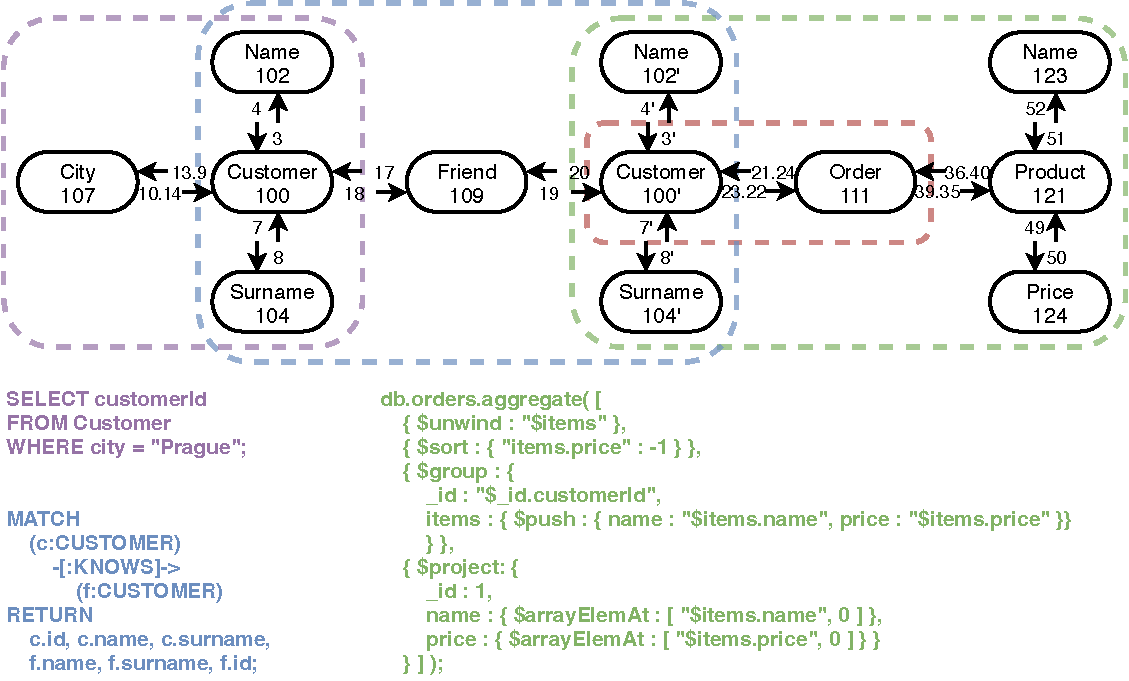
\includegraphics[width=\textwidth]{img/fig_query-decomposition.pdf} 
\caption{Query decomposition into relational (purple), graph (blue) and document (green) query parts, showing the corresponding generated native database queries for each query part~\cite{unified_representation}.}
\label{fig:querydecomposition}
\end{figure}

In~\cref{fig:querypullbacks}, we can then see how the categorical results for each query part will be joined together with pullbacks.
The first pullback joins the relational data with graph data ($P_1 = result_{REL} \bowtie_{100} result_{GRAPH}$), while the second one joins the document data with the result of the first pullback ($P_2 = P_1 \bowtie_{100'} result_{DOC}$).
As described in~\cref{algo:subsection:joinplan}, the join ordering problem is known to be hard, doubly so in multi-model scenarios, therefore it falls outside the scope of this thesis, and we leave it as part of future work on this topic.

\begin{figure}
\centering
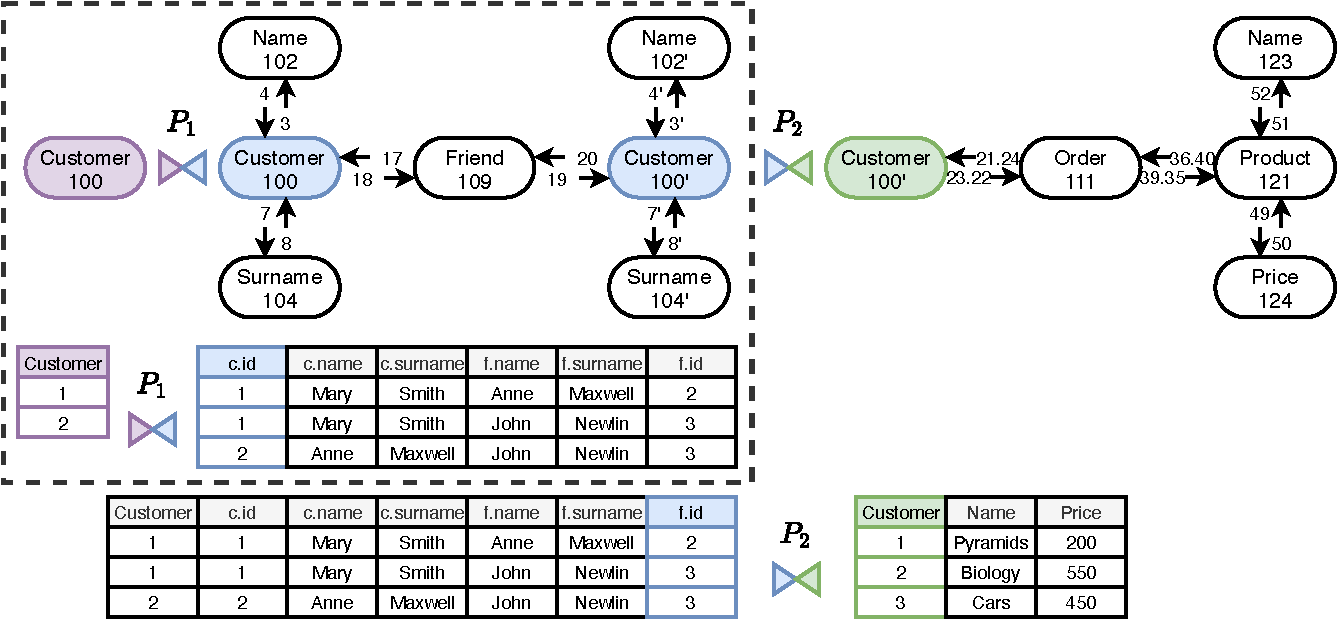
\includegraphics[width=\textwidth]{img/fig_query-join.pdf} 
\caption{Joining of query parts from~\cref{fig:querydecomposition} using pullbacks~\cite{unified_representation}.}
\label{fig:querypullbacks}
\end{figure}

\begin{figure}
\begin{code}
// PostgreSQL query
1,4,Alice
2,3,Bob
5,6,Charlie

// MongoDB query
{ customer_id: 1, price: 30 },
{ customer_id: 2, price: 25 },
{ customer_id: 3, price: 25 },
{ customer_id: 4, price: 30 },
{ customer_id: 5, price: 50 },
{ customer_id: 6, price: 10 }
\end{code}
\caption{Native query results for the queries shown in \cref{algo:fig:induced_native}.}\label{algo:fig:induced_results}
\end{figure}

For another example, we will remind the reader of the query in \cref{algo:fig:induced_query}.
Recall that in \cref{algo:fig:induced_native}, we showed the generated native queries for this MMQL query.
In \cref{algo:fig:induced_results}, we can see the results of these native queries as returned by the respective databases.
With these results, after their transformation to an instance category, we can expect to see the instance morphism $4_1$ to contain the following relations, showing relations between active domain rows of instance objects (each object active domain row is a set of tuples (signature, value)):

\begin{itemize}
    \item \texttt{(\{(6,30)\}, \{(1,1),(2,Alice)\})}
    \item \texttt{(\{(6,25)\}, \{(1,2),(2,Bob)\})}
\end{itemize}

As we can see in the first row, there is an order with a total price of $30$ which was placed by a customer with an ID of $1$ named Alice.
Let us also look at the instance morphism $4_2$:

\begin{itemize}
    \item \texttt{(\{(6,30)\}, \{(1,4),(2,Alice)\})}
    \item \texttt{(\{(6,25)\}, \{(1,3),(2,Bob)\})}
\end{itemize}

We can see that a different customer named Alice with an ID of 4 has also placed an order with a total price of $30$, and similarly, two different customers named Bob with IDs $2$ and $3$ have both placed an order with a total price of $25$.
There were also two customers named Charlie, but their orders do not have the same price, which is why they are excluded.

This approach for merging instance categories, coupled with the model-to-category transformation, leaves us with a single instance category representing the result of the MMQL \texttt{WHERE} clause.

\subsection{Projection}
\label{algo:subsection:projection}

With the instance category representing the result of the \texttt{WHERE} clause in hand, meaning we have already processed the selection part of the query, we also need to process the projection part, meaning the \texttt{SELECT} clause.
However, before we do that, there is one more thing which needs to happen -- \textit{execution of deferred statements}.
To get an overview of how this fits into the overall approach, we refer the reader to \cref{fig:queryworkflow}, whose Phase VI corresponds to the contents of this subsection.

\subsubsection{Deferred Statements}

As mentioned in~\cref{algo:subsection:transform}, there are certain MMQL statements which cross database boundaries, and therefore cannot be executed at the database level.
For example, we could have a \texttt{FILTER} statement demanding the equality of two variables whose values come from different databases.
Such statements must necessarily be processed by the MMQL query engine, and in the constraints of our approach where each query part is an executable unit independent of other query parts, this is unavoidable.
There is a possibility that for approaches which introduce dependencies between queries, a certain part of this may be optimized, for instance possibly adding a constraint to a query based on the results of another query.
However, as this is purely an optimization, we opted not to include this in our approach.

When it comes to the set of features which may possibly be a deferred statement, we have a few options, except for which all statements are \textit{not} deferred:

\begin{itemize}
    \item \textit{Triples} with repeated compound morphisms may be deferred statements in cases where the compound morphism being repeated crosses query part boundaries;
    \item \texttt{FILTER} statements may be deferred in cases where both operands of the included logic expression are variables or aggregations of variables, each of which is queried from a different database, or in cases where a required aggregation is not supported by the corresponding database; and
    \item \texttt{FILTER} and \texttt{VALUES} statements in query parts whose database wrappers define the \texttt{isNonIdFilterSupported} property to be false.
\end{itemize}

The processing of deferred statements essentially means their emulation by the query engine using the instance category corresponding to the query's \texttt{WHERE} clause.
We will not provide an explicit implementation of this algorithm, as its implementation would be lengthy and its inclusion in this thesis redundant, and all of the necessary operations are straightforward emulation of the statements.
Lastly, we will point out that the set of deferred (or deferrable) statements will vary depending on the design of the supporting algorithms for MMQL, as MMQL itself does not necessitate the deferral of any statements, opening the door to future optimizations.

\subsubsection{Projection Algorithm}

After the processing of deferred statements, we are ready to approach the main topic of this subsection, which is projection to the desired representation.
In this step, we take the instance category corresponding to the \texttt{WHERE} clause of the query, and transform it into an instance category corresponding to the \texttt{SELECT} clause, which induces its own schema category.
It is worth mentioning the construction of this schema category, as we will need the morphisms contained within to have correct cardinalities.
This can be achieved by iterating over the morphisms defined in the \texttt{SELECT} clause, and for each of them, finding all paths in the schema category induced by the \texttt{WHERE} clause between the subject and object of the triple where the morphism is defined, disregarding paths containing cycles.
We do not consider paths with cycles, as a cycle starting and ending with the same variable necessarily cannot have any effect on the cardinality of the final morphism, as it forms an identity function.
Note that there can indeed be multiple paths, for example if we consider two customers who each have a home address listed, we may have a query expressing the fact that both customers who ordered a specific item live at the same address, giving us two paths between the item ordered and the customer address.
For each morphism, we must examine all paths, selecting the minimal and maximal cardinality of the entire path, and then select the minimal value of the sets of minimal and maximal cardinalities to get the final minimal and maximal cardinality of the morphism.
This is because if multiple paths exist between the same two variables, a particular result will only be included in the instance category only if all of the paths match (unless some of those paths are optional and generated by the \texttt{OPTIONAL} clause, however we still need to consider them for the minimal and maximal calculation).
The algorithm generating the schema category induced by the \texttt{SELECT} clause can be seen in~\cref{algo:alg:projectionschema}.
We will point out the function \texttt{getPathsInSchema} used in line 10 of the aforementioned algorithm, which finds all paths in the schema category between two schema objects, provided to the function using the \texttt{src} and \texttt{dst} arguments for source and destination respectively.

\begin{algorithm}[ht]
\small
\DontPrintSemicolon
\SetKwProg{Fn}{function}{:}{}
\SetKw{return}{return}
\SetKw{break}{break}

\KwIn{$\mathbf{S}_{WHERE}$  -- schema category induced by the WHERE clause\;}
\myinput{$SELECT$  -- SELECT clause of the MMQL query\;}

$\mathbf{S}_{SELECT}$ := $\emptyset$

\ForEach{\textup{triple $subject$ $morphism$ $object$ in $SELECT$}}{
    \ForEach{\textup{$var$ in [$subject$, $object$]}}{
        $oldObj$ := $\mathbf{S}_{WHERE}$.getObjectFromVar($var$)
        
        $newObj$ := $\mathbf{S}_{SELECT}$.getObjectByKey($oldObj$.key)
        
        \If{\textup{$newObj$ is NULL}}{
            $\mathbf{S}_{SELECT}$.objects.add($oldObj$)
        }
    }

    $newMorphism$ := $\mathbf{S}_{SELECT}$.getMorphism($morphism$)

    \If{\textup{$newMorphism$ is NULL}}{
        $paths$ := getPathsInSchema($\mathbf{S}_{WHERE}$, src=$subject$, dst=$object$)

        \ForEach{\textup{$path$ in $paths$}}{
            \If{\textup{$path$ contains cycles}}{
                $paths$.remove($path$)
            }
        }

        $minCards$ := [ ]

        $maxCards$ := [ ]
        
        \ForEach{\textup{$path$ in $paths$}}{
            $minCards$.add(getMinCardinality($path$))
            
            $maxCards$.add(getMaxCardinality($path$))
        }

        $minCard$ := min($minCards$)

        $maxCard$ := min($maxCards$)

        $newMorphism$ := Morphism($morphism$, $subject$, $object$, $minCard$, $maxCard$)

        $\mathbf{S}_{SELECT}$.morphisms.add($newMorphism$)
    }
}

\caption{Projection Schema Algorithm.}
\label{algo:alg:projectionschema}
\end{algorithm}

With the schema category for the \texttt{SELECT} clause in hand, we can proceed to projecting the actual data, using the algorithm shown in~\cref{algo:alg:projectioninstance}.
This algorithm receives two inputs -- the instance category for the \texttt{WHERE} clause constructed in previous steps, and the schema category induced by the \texttt{SELECT} clause.
Its output is then data in the form of an instance category corresponding to the \texttt{SELECT} clause.
This algorithm copies over data from instance objects for the \texttt{WHERE} clause to instance objects for the \texttt{SELECT} clause (since variable projection does not modify the set of values).
It is worth explaining the notation \texttt{map($path$, $x$ $=>$ ...)} used on line 14 of \cref{algo:alg:projectioninstance}, which means the application of the lambda function in the second argument to \texttt{map} on each element of \texttt{$path$}.

\begin{algorithm}[ht]
\small
\DontPrintSemicolon
\SetKwProg{Fn}{function}{:}{}
\SetKw{return}{return}

\KwIn{$\mathbf{I}_{WHERE}$  -- instance category containing the results of the WHERE clause\;}
\myinput{$\mathbf{S}_{SELECT}$  -- schema category induced by the SELECT clause\;}

$\mathbf{I}_{SELECT}$ := $\emptyset$

\ForEach{\textup{$schemaObj$ in $\mathbf{S}_{SELECT}$.objects}}{
    $instanceObj$ := $\mathbf{I}_{WHERE}$.objects.getByKey($schemaObj$.key)

    $\mathbf{I}_{SELECT}$.objects.add($instanceObj$)
}

\ForEach{\textup{$schemaMorphism$ in $\mathbf{S}_{SELECT}$.morphisms}}{
    $subject$ := $schemaMorphism$.domain

    $object$ := $schemaMorphism$.codomain

    $paths$ := getPathsInSchema($\mathbf{S}_{WHERE}$, src=$subject$, dst=$object$)

    \ForEach{\textup{$path$ in $paths$}}{
        \If{\textup{$path$ contains cycles}}{
            $paths$.remove($path$)
        }
    }

    $instancePaths$ := [ ]

    \ForEach{\textup{$path$ in $paths$}}{
        $instancePath$ := map($path$, $x$ $=>$ getInstanceMorphism($x$, $\mathbf{I}_{WHERE}$))

        $instancePaths$.add($instancePath$)
    }

    $contractedPaths$ := map($instancePaths$, contractMorphisms)

    $instanceMorphism$ := baseInstanceMorphismIntersection($contractedPaths$)

    $instanceMorphism$.schemaMorphism := $schemaMorphism$

    $\mathbf{I}_{SELECT}$.morphisms.add($instanceMorphism$)
}

\caption{Projection Instance Algorithm.}
\label{algo:alg:projectioninstance}
\end{algorithm}

\begin{algorithm}[ht]
\small
\DontPrintSemicolon
\SetKwProg{Fn}{function}{:}{}
\SetKw{return}{return}

\KwIn{$instancePath$  -- list of base instance morphisms forming a path in the instance category induced by the WHERE clause\;}

$contractedPath$ := copy($instancePath$)

\While{\textup{len($contractedPath$) $> 1$}}{
    \tcp{If our path ends with morphisms (X) -a- (Y) -b- (Z), contract these morphisms to create a morphism (X) -a+b- (Z)}
    $b$ := $contractedPath$.popBack()

    $a$ := $contractedPath$.popBack()

    $joinedMappings$ := join($a$.mappings, $b$.mappings, $x_a$ $=>$ $x_a$.codomain, $x_b$ $=>$ $x_b$.domain)

    $contractedMappings$ := [ ]

    \ForEach{\textup{$joinedMapping$ in $joinedMappings$}}{
        $contractedMapping$ := $joinedMapping$.a.domain, $joinedMapping$.b.codomain

        $contractedMappings$.add($jcontractedMapping$)
    }

    $contractedMorphism$ := InstanceMorphism($contractedMappings$)

    $contractedPath$.add($contractedMorphism$)
}

\return{$contractedPath$.first()}

\caption{Function \texttt{contractMorphisms} from~\cref{algo:alg:projectioninstance}.}
\label{algo:alg:contractmorphisms}
\end{algorithm}

When it comes to creating the set of instance morphisms, it gets more complicated.
For morphisms from the \texttt{SELECT} clause which correspond to base morphisms from the \texttt{WHERE} clause, we can simply copy the instance morphism over to the new instance category, with a new signature corresponding to the signature specified in the \texttt{SELECT} clause.
However, it is possible for a morphism from the \texttt{SELECT} clause to correspond to a path (or set of paths) with length greater than one in the categorical representation of the \texttt{WHERE} clause.
In this case, we need to introduce the notion of \textit{morphism contractions}.
Given a compound morphism mapping a subject to an object, its contraction is a base morphism with the same mapping.
In other words, we merge the base morphisms which form the compound morphism into a single base morphism in the new instance category.
To do this, we must again get the set of paths (disregarding cycles) in the instance category induced by the \texttt{WHERE} clause, and perform morphism contraction on each path.
Finally, to produce the new instance morphism for the result instance category, we perform an intersection of all base morphisms created as a result of the path contractions, meaning the final domain-codomain map only contains a mapping of domain to codomain if all paths contain this mapping.

\subsubsection{Additional Considerations}

The perceptive reader may have noticed that the algorithm which we presented in \cref{algo:alg:projectioninstance} does not take into account the \texttt{OPTIONAL}, \texttt{UNION} and \texttt{MINUS} clauses of MMQL.
Indeed, the semantics of paths contained within these clauses are different in the context of creating result instance morphisms, however we intentionally omitted them from~\cref{algo:alg:projectioninstance} to preserve its simplicity and readability.

When it comes to paths within (or partially within) the \texttt{OPTIONAL} clause, we can disregard them if there exists at least one non-optional path, as the non-optional paths constrain the instance morphism to a set of mappings, and regardless of the existence of a particular optional mapping, the corresponding non-optional mapping always exists.
If no non-optional paths exist, then we define the instance morphism to be the union of all optional paths, after morphism contraction has been applied to them.
This is because for any given domain-codomain mapping to exist in the result instance morphism, it is enough for any given optional path to exist in the instance category corresponding to the \texttt{WHERE} clause.

Earlier, we specified that both arguments of the \texttt{UNION} clause are treated as optional.
If the entirety of a given \texttt{UNION} clause could be resolved within a single query part, we do not need to perform any extra work, as not only do we have the correct data in the instance morphisms, but the set of instance objects is also correctly filtered.
In the case that the \texttt{UNION} clause spans multiple query parts, we need to additionally filter the set of instance objects to eliminate those for whom neither \texttt{UNION} argument was matched.

As for the \texttt{MINUS} clause, the final instance morphism is the result of taking the instance morphism from the first argument of \texttt{MINUS}, while for any given domain-codomain mapping, if this mapping is also contained in the second argument of \texttt{MINUS}, it is eliminated.
Note that if the \texttt{MINUS} clause is contained entirely within a single query part, the required results have already been filtered out, meaning the filtering at this level is trivial, removing no mappings.

The last simplification made in the algorithm is the omission of constants and aggregations present in the \texttt{SELECT} clause.
While aggregations present here could be computed at the database level to increase overall efficiency, this is an optimization which would complicate the algorithms further, which is why we opted to simply explain it in this fashion.
Aggregations and constants in the \texttt{SELECT} clause would have schema objects defined just like variables, with corresponding instance objects having a constant value in the case of constants.
In the case of aggregations, their values would be computed according to their semantics as described in~\cref{mmql:subsection:grouping}, with the instance morphisms being defined accordingly.

We should also mention that the algorithms presented in this subsection are critical to query performance, as morphism contraction is an extremely expensive operation for a large dataset, entailing an inner join across all data in the instance morphism for each contraction.
The true cost of the contraction operation will be further explored in~\cref{eval}.

The final piece of the projection algorithm is taking care of the \texttt{ORDER BY}, \texttt{LIMIT} and \texttt{OFFSET} clauses of the query.
Again, while these could be handled at the database level natively, this is purely an optimization, and it would complicate the structure of our algorithms, which is why we opted to address them here.
As far as ordering is concerned, the final instance category would be divided up into maximal connected components, and these connected components ordered by the ordering criteria.
A special instance object would then be inserted into the instance category, with a morphism mapping sequence numbers from $1$ to $N$ to the connected components.
\texttt{LIMIT} and \texttt{OFFSET} are quite simple in their function, meaning we would simply restrict the result set as required.

To give a concrete example, recall the query from \cref{algo:fig:induced_query}, and the results of the generated native queries from \cref{algo:fig:induced_results}.
Given these results, the final instance category which represents the result of the MMQL query will have the following active domain rows for the \texttt{\_:shared} object:

\begin{itemize}
    \item \{(name,Alice),(price,30)\}
    \item \{(name,Bob),(price,25)\}
\end{itemize}

Again, note that each active domain row is a set of tuples (signature, value).
Normally when working with a schema category, base morphism signatures are integers which are automatically assigned, but technically a base morphism signature can be any string, which is why we allow their naming in the MMQL \texttt{SELECT} clause.

\subsection{Transforming Data}
\label{algo:subsection:transform}

As the result of the algorithm as proposed up to this point, we have an instance category corresponding to the schema category induced by the MMQL query's \texttt{SELECT} clause.
However, query results in the form of an instance category may not be practical for most use cases.
For this reason, we recognize the need for the query results to be transformed into a more suitable format, like JSON or RDF.
As MMQL is a categorical query language with categorical inputs and outputs, we believe that the transformation of data is best left out of the language itself, instead relying on supplemental query tooling to perform this job.
Despite this, we will describe our proposed approach for such a transformation, as we believe it is necessary to showcase the end-to-end validity and usability of the proposals made in this thesis.
This final part of the entire workflow corresponds to Phase VII as shown in \cref{fig:queryworkflow}.

In general, we can formalize this problem as the transformation of an instance category to a specific data model.
As we mentioned in~\cref{algo:subsection:joiningdata}, Pavel Koupil and Irena Holubov{\'a} proposed an algorithm for model-to-category transformation~\cite{unified_representation}, which we are using to transform data retrieved by native database queries into a categorical representation, and to subsequently join the data from multiple databases into a single instance category representing the \texttt{WHERE} clause of the MMQL query.
However, in the same paper, they also proposed an algorithm for a transformation in the opposite direction, meaning category-to-model (Algorithms 4 and 5 in their paper).
As it turns out, this algorithm solves exactly the problem we need to solve in order to transform the result instance category to a format like JSON or RDF.
For this reason, we propose that this algorithm be used for this transformation, and we refer the reader to the original source for more details on this algorithm.

It is worth mentioning that this transformation requires an input in the form of a mapping (recall~\cref{categorical:section:mapping}), which specifies the shape of the resulting data.
This mapping can be inferred from the shape of the MMQL \texttt{SELECT} clause in a straightforward way for some data models, for example in the graph model, we are simply transforming graph data to graph data in another representation, meaning relatively few modifications are necessary.
However, for some data models like the document model, this gets somewhat complicated.
The document model operates with tree structures, which in general do not permit lower levels of the tree to refer to upper levels.
This can pose a problem in the instance that the schema category induced by the \texttt{SELECT} clause contains back edges, forward edges or cross edges (borrowing terminology from the well-known Depth First Search algorithm), which was not an issue with graph data.

There are multiple possible solutions to the problem of transforming general directed graphs to trees~\cite{graph_tree_transform}, but we will mention two main approaches which are best suited to our use case.
The first approach is to automatically determine the schema object which will become the root of the tree, and construct a tree rooted in this schema object, replacing back, forward or cross references in the tree with object identifiers where possible, and with inlined data where not possible (for example with objects which have no identifier, such as JSON arrays).
The automatic determination of the tree root is simple in the case where the graph already forms a tree, but in the more general case, we would need to pick such a tree root based on an algorithm, for example one which would pick a tree root such that the number of edges in the tree preserved from the original graph is maximal.
The second approach would be to prompt the user to manually select the tree root when requesting a transformation which requires a root to be selected and the root cannot be determined automatically, for example when transforming to JSON when the schema category induced by the \texttt{SELECT} clause is not already a tree.
However, neither of the proposals is perfect as a transformation from a general graph to a tree necessarily carries some tradeoffs, which is why we believe that users of MMQL should try to formulate their queries to output categorical data in the shape of trees where possible.


% These chapters describe the actual implementation of what I programmed
\chapter{MM-quecat}
\label{quecat}

In the previous two chapters, we introduced MMQL, as well as the supporting algorithms enabling its implementation.
However, we presented both on a theoretical level only.
To properly evaluate the validity and correctness of our proposal, it must be verified in practice by way of implementation.
Therefore this chapter presents \textit{MM-quecat}\footnote{\url{https://github.com/yawnston/querycat}}, a proof-of-concept implementation of the core concepts of MMQL.
The purpose of this implementation is the verification of our proposed approach. Full implementation of all MMQL concepts for all scenarios would be beyond the scope of this thesis, which is why the implementation focuses only on the key parts of MMQL.
This chapter not only describes the implementation of MM-quecat itself, but also the technical challenges faced along the way.

\section{Solution Architecture}

MM-quecat is a Python 3\footnote{\url{https://www.python.org/}} library which provides the functionality of executing MMQL queries.
Its interface is rather simple on the surface - it provides a function \texttt{execute\_query}, which takes the input query as a string, and returns an instance category (see~\cref{categorical:section:instance}) representing the result of the query.

To do this, it needs to communicate with MM-evocat~\cite{evocat}, which is a multi-model data modeling and evolution framework based on category theory, written as a Java server application.
MM-evocat has the functionality of creating a schema category (see~\cref{categorical:section:schema}).
For that reason, MM-quecat's main interface function \texttt{execute\_query} also contains a parameter containing the ID of the schema category, which refers to a schema category within MM-evocat.
In MM-evocat, one can not only model the schema category, but also create the mappings necessary to transform data from its native representation into the categorical representation, using an algorithm for model-to-category transformation~\cite{unified_representation}.
While including MM-evocat in the solution does introduce overhead in the form of network communication, the benefits it brings outweigh the negatives for our purposes, since it includes the categorical modeling tools which are necessary for MM-quecat to do its job.
Without MM-evocat, MM-quecat would need to implement all of the necessary functionality itself, effectively duplicating the functionality of MM-evocat to avoid network overhead, which is not desirable at this point of the tool's lifecycle as proof-of-concept software.
MM-evocat is also still in active development by its author and is not yet fully finished, which further complicates its usage, as we will mention again going forward in this chapter.
Perhaps in the future, if the a full and optimized implementation of MM-quecat is desired and when MM-evocat's development is finished, both tools could be merged into a single one.

\begin{figure}[h]
\centering
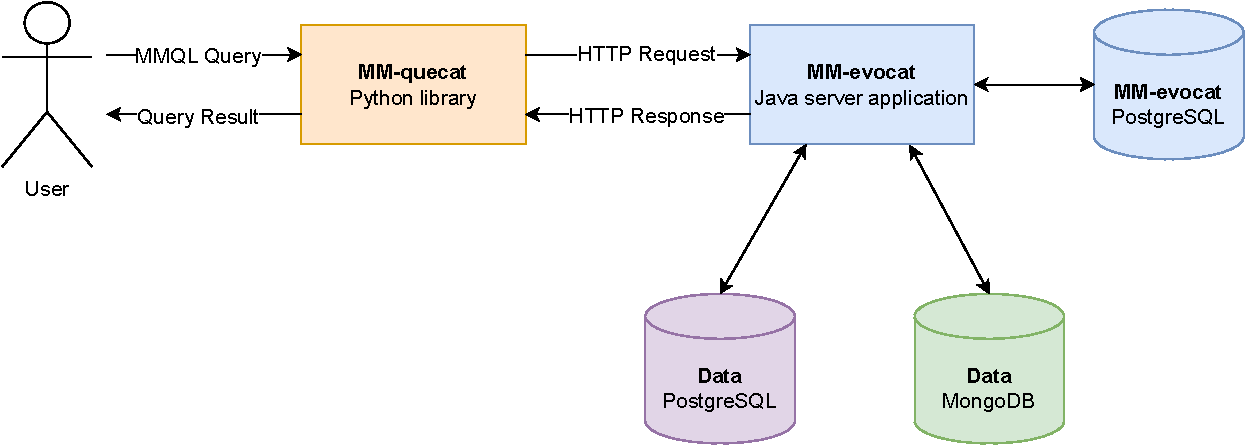
\includegraphics[width=\textwidth]{img/quecat-architecture.pdf} 
\caption{Architecture of the MM-quecat solution.}
\label{fig:quecatarchitecture}
\end{figure}

The architecture of the whole solution can be seen in~\cref{fig:quecatarchitecture}, which shows MM-quecat communicating with MM-evocat via HTTP.
We can see that MM-quecat sends requests to an instance of MM-evocat which contains the necessary schema category and mappings representing the data being queried, as well as maintaining the connections to the relevant databases.
Note that at no point does MM-quecat actually need to communicate with the queried databases directly, as the queries generated by MM-quecat are passed to MM-evocat, which executes the queries and transforms their results to the categorical representation using a mapping provided by MM-quecat\footnote{While direct database communication is not necessary in MM-quecat's current form, the implementation of a fully-featured multi-model query planner would necessitate this direct connection, as the query planner would need access to the databases' own query planners, usually in the form of a database explain command, to assess the cost of MMQL multi-model query plans.}.
This increases the modularity of the solution, as MM-quecat only needs to rely on the categorical interface of MM-evocat, and the database wrappers (recall~\cref{algorithms:subsection:wrappers} where we introduced the notion of database wrappers) have their implementation greatly simplified, as they only need to generate the native queries without having to worry about executing them, or transforming their results to a categorical representation\footnote{A potential problem may arise if the database wrappers need to access the database interface to query it for the supported query language version in cases where the database wrapper is deciding whether it may use a newer language feature. However, this would be solved by simply adding the database connection to MM-quecat just like in the case of the query planner.}.
Lastly,~\cref{fig:quecatarchitecture} shows that MM-evocat also has its own PostgreSQL database which it uses to store schema and mapping data, as well as instance categories.
This database is separate from the databases containing the actual data being queried.
Going forward, MM-quecat will also be wrapped in a simple HTTP API as required for the purposes of the querying tool which we will introduce in~\cref{querytools}, as this querying tool will continue being worked on as part of a conference demo paper which the author of this thesis is co-authoring~\cite{mm_quecat}.

For completeness, we should also mention the choice of Python as the language for the implementation of MM-quecat.
The ecosystem of tools developed for multi-model data representation at the Faculty of Mathematics and Physics of Charles University, which MM-quecat and MM-evocat are a part of, already contains projects in both Java and Python, making both languages natural candidates for the cohesion of the tool ecosystem.
From these two languages, Python was chosen due to the personal preferences of the author of this thesis, as they have extensive experience with Python, but little to no Java experience.
To add to this, it is the author's personal belief that Python, with its simplicity, ease of use and universal usefulness, is the language of the future, and will continue to gain market share while Java slowly fades away to make room for more modern languages.

Since MMQL is a multi-model query language and MM-quecat is a library implementing MMQL, we also need to discuss MM-quecat's multi-model capabilities.
As implemented, MM-quecat supports two models - relational in the form of PostgreSQL, and document in the form of MongoDB.
The reason for this is relatively straightforward, as both databases are among the most popular in their class, and together they represent a significant market share of the database space.
In addition, MM-evocat currently only supports these two databases, which means that MM-quecat cannot support additional databases without their corresponding implementation in MM-evocat.
Among other limitations, MM-evocat only supports string values, meaning the data type of everything in MM-evocat is a string.
For this reason, MM-quecat is also constrained to only supporting strings, even though MMQL also supports other data types.

With the solution architecture out of the way, we will describe specific parts of MM-quecat and their implementation, loosely following the solution structure proposed in~\cref{algorithms:section:approach}.

\section{Parsing}

The first step in implementing any language, be it a query or programming language, is to implement a parser for this language.
This is because it is not feasible to work with a language based on its raw text alone, but rather it is more practical to operate on language-level constructs which are parsed from the raw text by a parser.
While the parser for MMQL could be manually implemented, a smarter solution exists in the form of parser generators.
These tools generally accept some sort of formal grammar as input, and in return generate a parser for the language represented by the grammar.
As it happens, we had been planning to formally specify the grammar of MMQL anyway, which made using the grammar to generate a parser a natural step.
The grammar used to generate the parser for MM-quecat is included  in~\cref{attachment:grammar}.

This was accomplished using the ANTLR\footnote{\url{https://www.antlr.org/}} library, which is a parser generator for reading, processing, executing, or translating structured text or binary files.
ANTLR was used to generate the parser classes in Python, at which point we implemented an abstract syntax tree (AST) visitor, which walks the AST created by the generated parser, and converts it into a suitable form for further processing in the query execution process.
This form consists of translating the input graph patterns into sets of triples, coupled with additional constructs such as \texttt{FILTER} expressions or other query features.

\section{Creating Query Plans}

As described in~\cref{algorithms}, we need to divide the query up into query parts to form query plans.
First, queries are preprocessed to transform triples containing compound morphisms into multiple triples, each containing a base morphism.
For each point where a compound morphism was split, a temporary internal variable is inserted into the query.
As discussed in~\cref{algorithms:subsection:preprocessing}, this greatly simplifies query processing as a whole, but introduces issues when it comes to performance and recursive paths.
The performance consideration is not an issue for MM-quecat, as achieving high performance is not within the scope of its proof-of-concept nature (and within the scope of this thesis in general).
The consideration of recursive morphisms, while unpleasant, is also not key to demonstrating the viability of MMQL and MM-quecat as a whole.
The implementation of recursive morphisms would also be rather complex, which is why they are not supported in the implementation, giving us space to focus on the main focus points of this thesis.

Aside from the preprocessing, the implementation of query plan creation largely copies the algorithm outlined in~\cref{algo:subsection:queryplan}, which is why we will not discuss it here further.

\section{Query Translation}

The query translation algorithm is a simplified, limited version of the algorithm presented in~\cref{algo:subsection:translation}, supporting simple queries with both base and compound morphisms.
However, the scope of the implementation of this algorithm is not limited only by the implementation effort required.
As we mentioned earlier in this chapter, MM-evocat is still undergoing active development by its author, and as a consequence, some of its features are not quite finished yet.
For example, there is an issue where if MM-quecat generates queries requiring database joins on multiple kinds (like multiple tables in the relational model or multiple collections in the document model), MM-evocat will not correctly process these queries when translating their results into the categorical representation, yielding an incorrect instance category.
For this reason, MM-quecat cannot support queries with multiple kinds in a single query part at this time.
While this is bothersome in terms of the completeness of the implementation, it is not an issue in the scope of a proof-of-concept implementation, as we can demonstrate the multi-model capabilities of MM-quecat on multi-model queries which do not require the use of multiple kinds from the same database.
One such query is later shown in~\cref{fig:evalmultimodelmmql} while evaluating the weaknesses of MM-quecat.

\section{Selecting the Best Query Plan}

In~\cref{algo:subsection:bestplan}, we discussed the difficulties which come with multi-model query planning, and the lack of related work on the subject, with most sources only considering single-model query planning within the context of a single database.
For that reason, in~\cref{algo:subsection:bestplan} we left the selection of the best query plan as an open point which is beyond the scope of this thesis, which already breaches the vast and complex area of multi-model querying with little related work to use as a base.
Therefore in MM-quecat, the implementation of best plan selection is purposefully very basic - an arbitrary query plan is selected if multiple plans are present due to data redundancy.
The implementation of a more sophisticated selection process first necessitates additional research on possible approaches to this problem.

\section{Query Execution}

As discussed earlier in this chapter, MM-evocat has the ability to execute native database queries in PostgreSQL and MongoDB, and then transform their results into the categorical representation.
It also has the ability to merge the results of multiple such queries over the same schema category into a single instance category, using the objects' identifiers to determine the proper way to join the data.
However, MM-evocat does not have the ability to execute arbitrary queries as required by MM-quecat, and its capability is limited to trivial projection-only queries that exactly copy the structure of the defined mappings.
This is an issue, because MM-quecat generates various queries, which then need to be executed against the databases.

Because MM-evocat is in active development, waiting for MM-evocat to support this arbitrary query execution was not realistic within the context of this thesis.
This is why MM-quecat is actually using a modified instance of MM-evocat\footnote{\url{https://github.com/yawnston/evolution-management}}, which was forked from the main implementation, in which the author of this thesis has made the modifications necessary for MM-quecat to fully function.
The modifications include, but are not limited to:

\begin{itemize}
    \item Modifying the API to allow execution of arbitrary database queries;
    \item Modifying the database wrappers for PostgreSQL and MongoDB to execute the provided queries, including the ability for the MongoDB wrapper to execute aggregation pipelines instead of simple find queries;
    \item Modifying the API to allow the retrieval of instance morphisms, in addition to the retrieval of instance objects, which was already implemented; and
    \item Addition of Docker\footnote{\url{https://www.docker.com/}} configuration files to easily run MM-evocat, since its setup is not very straightforward and includes multiple components.
\end{itemize}

For this reason, MM-quecat only functions with the modified version of MM-evocat.
However, in the future, when MM-evocat is modified by its author to fully support the features required by MM-quecat, these temporary modifications will become obsolete, and MM-quecat will use the main, up-to-date MM-evocat.

Aside from the necessity for these modifications, the query execution algo\-rithm operates mostly as described in~\cref{algorithms}.
MM-quecat uses the API provided by MM-evocat to create a copy of the queried schema category, and to define the mappings which are needed by the query parts in the query.
These mappings define the shape of the results of each individual native database query, effectively telling MM-evocat how to transform the result of this query into the categorical representation.
The queries generated by MM-quecat are executed within MM-evocat, including joining of their results into a single instance category.
This instance category is then retrieved from MM-evocat using the modified API, and the remaining steps are executed as described in~\cref{algorithms}, projecting the instance category to the final instance category, along with creating the schema category defining this result instance category.
The final instance category is then returned as the result of the query.

Note that in our description of the proposed approach in~\cref{algorithms:section:approach}, we also mentioned the need to transform the query result into a more usable representation, such as JSON.
We discussed this in greater detail in~\cref{algo:subsection:transform}, where we mentioned the fact that we can use an existing algorithm for category-to-model transformation~\cite{unified_representation}.

This is another limitation where MM-evocat is not quite ready, as this functionality is not yet fully implemented as required by MM-quecat\footnote{In particular, the algorithm for category-to-model transformation itself is implemented, but not the relevant functionality for the transformation to a format like JSON or RDF.}.
However, when the required functionality is complete on the side of MM-evocat, MM-quecat will take the schema category corresponding to the query result, define the required mappings to transform the result into a JSON representation, and send both over to MM-evocat to perform the actual transformation.

As a whole, the implementation of MM-quecat in this form is sufficient to verify the validity of our proposed approach, as we later demonstrate in~\cref{eval} with concrete queries processed by MM-quecat.
However, as can be seen from the solution architecture, there is certainly room for performance optimization, since there is quite a bit of network communication overhead between MM-quecat and MM-evocat, along with the proposed algorithms being optimized for readability and simplicity, not performance.
These considerations will also be discussed in~\cref{eval}.

\chapter{Querying Tools}
\label{querytools}

In the previous chapter, we discussed the proof-of-concept implementation of MM-quecat, which exists in the form of a Python library.
However, despite its interface being easy to use, it does not fully leverage the power of MMQL with respect to the end user experience.
Recall that in~\cref{category:section:querylanguage}, we articulated the requirements that MMQL \textit{be expressive and readable}, and that it \textit{be intuitive and familiar to users of existing query languages}.
While we believe that MMQL meets these design goals as proposed, and that one of its greatest strengths lies in being graphically expressive, meaning users can define graph patterns which visually resemble the actual structures being defined.
Therefore, in this chapter, we present the prototype of a user interface (UI) application for MM-quecat\footnote{\url{https://github.com/yawnston/quecat-frontend}}, which allows the user to visually construct queries.

The presented prototype is not one of the main products of this thesis, but we present it regardless, as it should give the reader an idea of how the language may be used from an end-user perspective.
The prototype of the UI for MM-quecat was created by the author of this thesis while working on a not-yet-published demo paper~\cite{mm_quecat}, co-authored with Pavel Koupil and Irena Holubov{\'a}.
Therefore its implementation will be completed as the paper nears its publishing date, and in this chapter, we present it as it exists in its current form.

The querying tool is a web application built with React\footnote{\url{https://reactjs.org/}} and Next.js\footnote{\url{https://nextjs.org/}}, utilizing the Cytoscape.js\footnote{\url{https://js.cytoscape.org/}} library for graph visualization and MUI\footnote{\url{https://mui.com/}} as a component library.

\section{Requirements}

Before we introduce our design, we first need to formalize the requirements for such an application.
The application should primarily serve as a querying tool, meaning it should be possible for the user to construct a query using the schema category as a visual aid.
The user should have the ability to directly execute the query, and retrieve the results in the chosen representation (like JSON for example).

Aside from this primary use case, the user should also have the ability to view all of the possible query plans created by MM-quecat for the execution of the query.
Each query plan should be able to be examined further, displaying the native database queries generated by MM-quecat for this specific query plan, as well as visualizing the query plan in a subset of the full schema category.

As a whole, the query tool should heavily leverage the graphical nature of MMQL, nicely visualizing the query in the schema category and possibly even providing semantic syntax highlighting in the query itself, with colors corresponding to the concepts visualized in the schema category.

\section{User Interface}

Now that we have formalized the requirements for a MMQL query tool, we will showcase our prototype.
The main query screen can be seen in~\cref{fig:uiquery}, where on the right side, the user may construct an MMQL query, and on the right side, a visual aid in the form of the schema category is present.
To help the user understand the query that they are writing, the schema category display also contains a visualization of various query features.

\begin{figure}[h]
\centering
\shadowimage[width=.95\textwidth]{img/quecat-ui-query.png} 
\caption{MM-quecat querying UI, showing the query on the right, and the schema category with the visualized query on the left.}
\label{fig:uiquery}
\end{figure}

For example, the \texttt{Order} schema object is colored blue, as it lies on the query path, but is not a part of the projection.
The \texttt{Contact} object is colored gray since it is not part of the query at all, and the \texttt{Name} object corresponding to a \texttt{Product} is colored purple, since it is part of the query projection.
Lastly, we can see that the \texttt{Name} object corresponding to a \texttt{Customer} is colored purple with an orange outline, meaning that it is part of the projection, and there exists a filter on this schema object.

If the application user clicks on the "EXPLAIN" button in the bottom part of the screen, they will be taken to the screen shown in~\cref{fig:uiplans}.
There they can see a list of all possible query plans, coupled with their plan cost and the databases used in the plan.

\begin{figure}[h]
\centering
\shadowimage[width=.95\textwidth]{img/quecat-ui-plans.png} 
\caption{A table displaying all query plans generated by MM-quecat and their details.}
\label{fig:uiplans}
\end{figure}

The user may further examine individual query plans, leading to the screen shown in~\cref{fig:uidetail}.
This screen, similarly to the screen shown in~\cref{fig:uiquery}, shows the schema category on the left side, however in this instance, the schema category is restricted to the databases and schema objects which are part of this specific query plan.
On the right side, the user can see the native database queries which were generated for this plan by MM-quecat.
The user can use this information to verify that the queries generated by MM-quecat are, for instance, using the correct indexes in the corresponding databases.

\begin{figure}[h]
\centering
\shadowimage[width=.95\textwidth]{img/quecat-ui-detail.png} 
\caption{Detailed view of a specific query plan, showing the native database queries generated by MM-quecat.}
\label{fig:uidetail}
\end{figure}

\chapter{Evaluation}
\label{eval}

Now that we have discussed the goals and scope of the proof-of-concept implementation of MM-quecat, recall that in~\cref{quecat}, we mentioned query performance as one of the main open points of our approach.
In~\cref{category:section:querylanguage}, we mentioned that a suitable multi-model query language should \textit{"have the capability of being nearly as performant as native queries where possible"}.
To that end, we discussed optimization options in~\cref{algorithms} while discussing the proposed algorithms.
However, in order to properly understand the performance of the proposed approach, and to be able to constructively suggest effective optimizations for the future, it would be useful to experimentally evaluate the performance of MM-quecat.
This chapter is therefore dedicated to such an evaluation.

Specifically, we have four main goals in mind for the experiments in this chapter, which is to:

\begin{enumerate}
    \item Understand the overhead introduced by our approach compared to native database queries in a single-model scenario;
    \item Understand the overhead in the context of merging data in a multi-model, multi-database scenario;
    \item Locate the main performance bottlenecks in MM-quecat; and
    \item Establish a performance baseline for future optimizations.
\end{enumerate}

The motivations for the first goal should be quite clear, as our approach introduces overhead in the form of converting data into a categorical representation and network communication overhead.
Therefore to properly fulfill the first goal of this chapter, we will need to prepare simple, single-model scenarios which we can use to isolate the amount of overhead introduced in this fashion.

As for the second goal, recall that in~\cref{algorithms}, we mentioned the need to merge together data retrieved from different query parts.
While the merging itself is not performed directly by MM-quecat, but rather by MM-evocat~\cite{evocat}, it is still crucial to understand the impact of this step on the whole approach.
To this end, we will naturally need to include a multi-model scenario in our evaluation.

Lastly, a simple observation motivates the third goal - in practice, it is best to avoid premature optimization, and rather use benchmarking to identify specific performance bottlenecks.
Because the problem domain of multi-model querying is very complex, naturally the approaches we designed are as well.
This means that avoiding premature optimization is even more important, as we want to preserve the simplicity and comprehensibility of our approach where possible.
To this end, during the writing of this chapter, two key tools were utilized to aid us in locating performance bottlenecks: Python's cProfile\footnote{\url{https://docs.python.org/3/library/profile.html}} module which allows us to collect performance statistics about Python programs, and SnakeViz\footnote{\url{https://jiffyclub.github.io/snakeviz/}}, which is a tool for the visualization of cProfile's output.

Before we begin with the evaluation itself, it is also worth mentioning that the use cases designed for evaluation purposes also serve as use cases for the verification of the implementation of MM-quecat.
Specifically, the multi-model use case presented in~\cref{eval:section:multimodel} also presents the main use case of MM-quecat (and this thesis in general), which is the unified querying of multi-model data.
By including this use case in the evaluation, we also verify that MM-quecat fulfills its intended primary purpose.

\section{Evaluation Framework}

\begin{figure}[h]
\centering
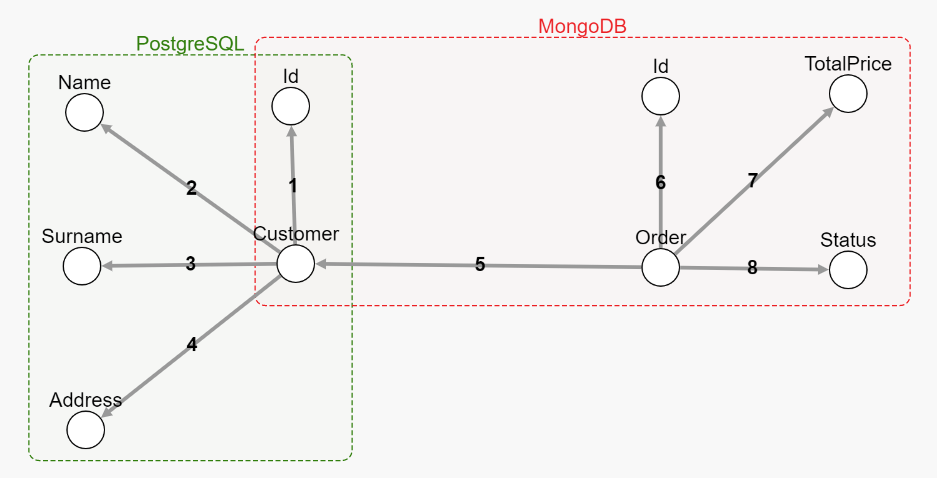
\includegraphics[width=\textwidth]{img/eval-category.png} 
\caption{Schema category used for all evaluations.}
\label{fig:evalcategory}
\end{figure}

For the purposes of the aforementioned evaluations, we propose a model scenario used for both single-model and multi-model evaluations.
The schema category for this scenario is shown in~\cref{fig:evalcategory}.
The corresponding mappings are then shown in~\cref{fig:evalmapping}.
The customers along with their properties are stored in a PostgreSQL table, and the orders are stored in a MongoDB collection.
Using this schema, we are able to easily test the multi-model functionality of MM-quecat while keeping the example simple and understandable.
Note that the \texttt{customer\_id} stored for each order in MongoDB refers to a customer stored in PostgreSQL, allowing the joining of the data.

For each evaluation scenario, the given MMQL query is executed, timed, and its execution time is compared to the execution time of a native database query (or two native queries in the case of the multi-model scenario).
Each scenario was repeated 100 times, and the presented results are the average of all repetitions.

The choice of databases for this example scenario is also not random - MM-evocat~\cite{evocat} supports only PostgreSQL and MongoDB, and therefore MM-quecat does as well.
Therefore the only reasonable option is to use both the supported databases if we want to examine the multi-model behavior.

\begin{figure}[h]
\centering
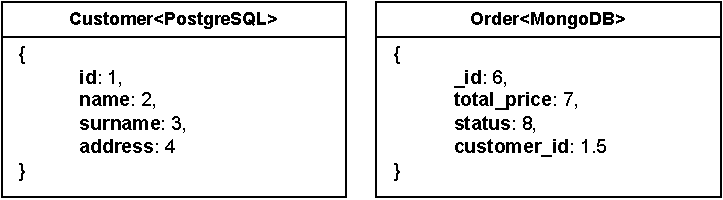
\includegraphics[width=\textwidth]{img/eval-mappings.pdf} 
\caption{Mappings corresponding to the schema category in~\cref{fig:evalcategory}.}
\label{fig:evalmapping}
\end{figure}

Every proper test needs a well-defined set of input data, and it is no different for our case.
The data was generated using the Faker\footnote{\url{https://faker.readthedocs.io/en/master/}} library, using a random seed for reproducibility.
As for the size of the data, a set of 2000 customers and 6000 orders was used, with each customer being assigned 3 orders.

The evaluations were performed on a laptop with an 11th generation Intel i7 CPU, 32 gigabytes of operating memory and an SSD.
Both databases as well as the MM-evocat instance were running locally on the same machine, using Docker\footnote{\url{https://www.docker.com/}} for virtualization.

It is also worth reminding that even though there is a single multi-model schema for all evaluations, we are able to use specific parts of it for the single-model evaluations.

All evaluations described in this chapter are part of the MM-quecat source code\footnote{\url{https://github.com/yawnston/querycat}} as executable Python scripts in the \texttt{src/experiments} folder.

\section{Single-Model Evaluation}

As mentioned in the introduction of this chapter, the purpose of single-model evaluation is to isolate the overhead introduced by our approach compared to native database queries.
In a single-model scenario, we do not need to consider the overhead of merging together data from multiple different databases, and we can focus on only the base overhead.
A separate evaluation was carried out for both currently supported databases - PostgreSQL and MongoDB.

\subsection{PostgreSQL}
\label{eval:subsection:postgresql}

In the PostgreSQL evaluation, let us consider a query which simply selects all customers along with their properties, using the schema shown in~\cref{fig:evalcategory}.
Such a MMQL query is shown in~\cref{fig:evalpostgresqlmmql}.

\begin{figure}[ht]
\begin{code}
SELECT {
    ?customer id ?id ;
        name ?name ;
        surname ?surname ;
        address ?address .
}
WHERE {
    ?customer 1 ?id ;
        2 ?name ;
        3 ?surname ;
        4 ?address .
}
\end{code}
\caption{MMQL query used for PostgreSQL single-model evaluation.}\label{fig:evalpostgresqlmmql}
\end{figure}

We also consider an equivalent PostgreSQL query shown in~\cref{fig:evalpostgresqlnative}, which was used as the benchmarking query.
When compared to the query shown in~\cref{fig:evalpostgresqlgenerated}, which was internally generated by MM-quecat for the given MMQL query, we can see that they are functionally identical.

\begin{figure}[ht]
\begin{code}
SELECT id, name, surname, address
FROM experiments_customers
\end{code}
\caption{PostgreSQL query used for benchmarking performance.}
\label{fig:evalpostgresqlnative}
\end{figure}

\begin{figure}[ht]
\begin{code}
SELECT 
  experiments_customers.id AS experiments_customers_id, 
  experiments_customers.name AS experiments_customers_name, 
  experiments_customers.surname AS experiments_customers_surname, 
  experiments_customers.address AS experiments_customers_address 
FROM 
  experiments_customers
\end{code}
\caption{PostgreSQL query generated by MM-quecat from the query shown in~\cref{fig:evalpostgresqlmmql}.}
\label{fig:evalpostgresqlgenerated}
\end{figure}

The results of this evaluation scenario can be seen in~\cref{table:evalpostgresqlresults}, with the first row showing the raw elapsed query time in milliseconds, and the second row showing slowdown relative to the native query.
We can see that on average, the MMQL query took a little over 1 second to execute, compared to just 4ms for the native query, giving us a slowdown of roughly 288 times.

\begin{table}[h!]
\centering
\begin{tabular}{l@{\hspace{1.5cm}} c c}
& \textbf{Native Query} & \textbf{MM-evocat} \\
\midrule
Elapsed Time & 4ms & 1153ms \\
Slowdown & 1x & 288x \\
\bottomrule
\end{tabular}
\caption{Average query time measurements for the single-model PostgreSQL scenario.}\label{table:evalpostgresqlresults}
\end{table}

This degree of slowdown was within the realm of expectation, because we need to consider the overhead of communication with the MM-evocat instance, as well as the overhead of transforming the data into a categorical representation.
However, what is more interesting is to take a look at where the majority of the slowdown is coming from.
Looking at~\cref{fig:evalpostgresqlprofile}, we can see performance measurement data collected by cProfile and visualized by SnakeViz\footnote{The profiler run was done separately from the performance measurement runs shown in~\cref{table:evalpostgresqlresults} in order to eliminate any possible performance effect of the profiler itself.}.
This data shows a visualization of the total execution time spent in given function calls, starting at the top and decomposing the function calls further as we go down in the image.

\begin{figure}[h]
\centering
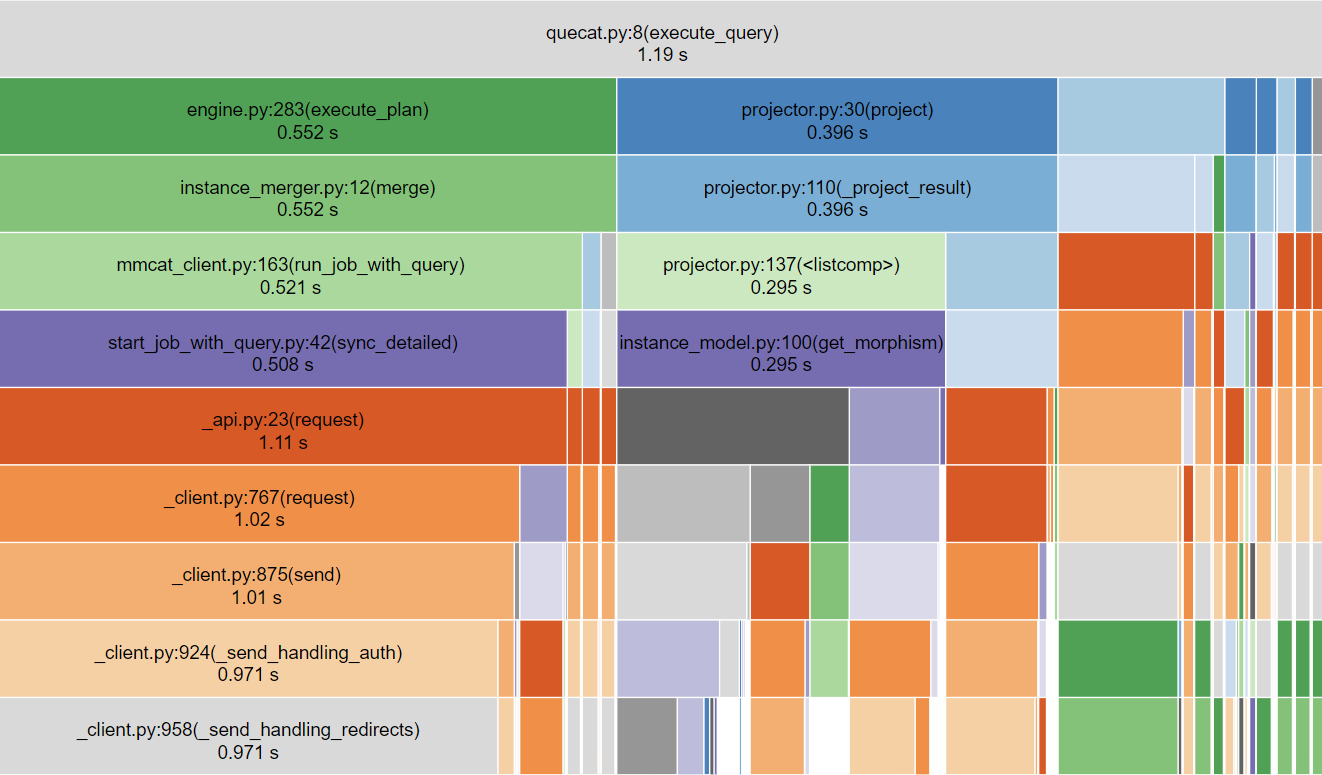
\includegraphics[width=\textwidth]{img/eval-postgre-profile.png} 
\caption{Profiler data for the single-model PostgreSQL scenario.}
\label{fig:evalpostgresqlprofile}
\end{figure}

Some function names are omitted from the image due to the available space, but examining the data contained within reveals the main takeaway of this evaluation scenario: the majority of the time was spent on \textbf{network communication} with MM-evocat.
This network communication necessarily includes the transfer of all retrieved data from MM-evocat to MM-quecat.
In other words, the amount of time spent otherwise manipulating the data was trivial.
This gives us a good baseline idea of the performance of MM-quecat, as we can expect that execution times for arbitrary queries will likely not go too far below 1 second.

The only feasible way of reducing this overhead further would be to revise the architecture of the ecosystem including MM-evocat and MM-quecat, and to merge them together into a single tool.
However, that would be far from trivial, considering the relevant tools were developed independently as part of different theses using different languages. Such an endeavor may not be worth the performance benefits at this point of the tools' lifecycle.
Perhaps if in the future a highly performant variant of both MM-evocat and MM-quecat is desired, a new, unified tool can be built from scratch using the knowledge gained from the design and implementation of both tools.

\subsection{MongoDB}
\label{eval:subsection:mongodb}

Similarly to~\cref{eval:subsection:postgresql}, this evaluation scenario evaluates MM-quecat in the context of a single data model within a single database.
The evaluated MMQL query for this scenario is shown in~\cref{fig:evalmongodbmmql}, the benchmark MongoDB query is shown in~\cref{fig:evalmongodbnative}.
The query generated by MM-quecat is identical to the query shown in~\cref{fig:evalmongodbnative}, therefore it is not shown in a separate figure.

\begin{figure}[ht]
\begin{code}
SELECT {
    ?order id ?orderId ;
        totalPrice ?totalPrice ;
        status ?status ;
        customerId ?customerId .
}
WHERE {
    ?order 6 ?orderId ;
        7 ?totalPrice ;
        8 ?status ;
        5/1 ?customerId .
}
\end{code}
\caption{MMQL query used for MongoDB single-model evaluation.}\label{fig:evalmongodbmmql}
\end{figure}

\begin{figure}[ht]
\begin{code}
db.experiments_orders.aggregate([
    {
        "$project": {
            "_id": 1,
            "total_price": 1,
            "status": 1,
            "customer_id": 1
        }
    }
])
\end{code}
\caption{MongoDB query used for benchmarking performance, identical to the query generated by MM-quecat.}
\label{fig:evalmongodbnative}
\end{figure}

The results of this evaluation scenario can be seen in~\cref{table:evalmongodbresults}.
We can see that the average execution time for the native MongoDB query was 16ms, while the average for MM-evocat was 5458ms.
This gives us an approximate slowdown of 341x.

\begin{table}[h!]
\centering
\begin{tabular}{l@{\hspace{1.5cm}} c c}
& \textbf{Native Query} & \textbf{MM-evocat} \\
\midrule
Elapsed Time & 16ms & 5458ms \\
Slowdown & 1x & 341x \\
\bottomrule
\end{tabular}
\caption{Average query time measurements for the single-model MongoDB scenario.}\label{table:evalmongodbresults}
\end{table}

The measurements show an increase in the overhead incurred by MM-evocat, and the reason for this becomes apparent when examining~\cref{fig:evalmongodbprofile}.
As we can see, network communication between MM-evocat and MM-quecat now only takes up approximately 30\% of the total query execution time.
The remaining 70\% is taken up by work being done in the \texttt{QueryProjector} class, specifically by the method \texttt{\_contract\_morphisms}.

Recall that in~\cref{algo:subsection:projection}, we discussed the projection algorithm, including the need for so-called morphism \textit{contractions}.
A morphism contraction is an operation on the instance category, where we may need to contract multiple instance morphisms into a single one because of the required projection in the query.
This is an operation which for $m$ morphisms with data size $n$ effectively requires $m-1$ joins between instance morphism domain rows, where each instance morphism may contain up to $n$ domain rows.
These joins are implemented using a linear number of operations and a hash table in MM-quecat, however there may be room for optimization here.
Perhaps a more efficient contraction algorithm could be designed, eliminating the need for hashing by clever usage of memory layout for the data being joined.
Similarly, the representation of the instance category is not optimized for performance, therefore there may be some room for improvement here as well.
In any case, the instance morphism contractions form a major performance bottleneck in MM-quecat, along with the serialization and deserialization of the instance category also having room for optimization.

\begin{figure}[h]
\centering
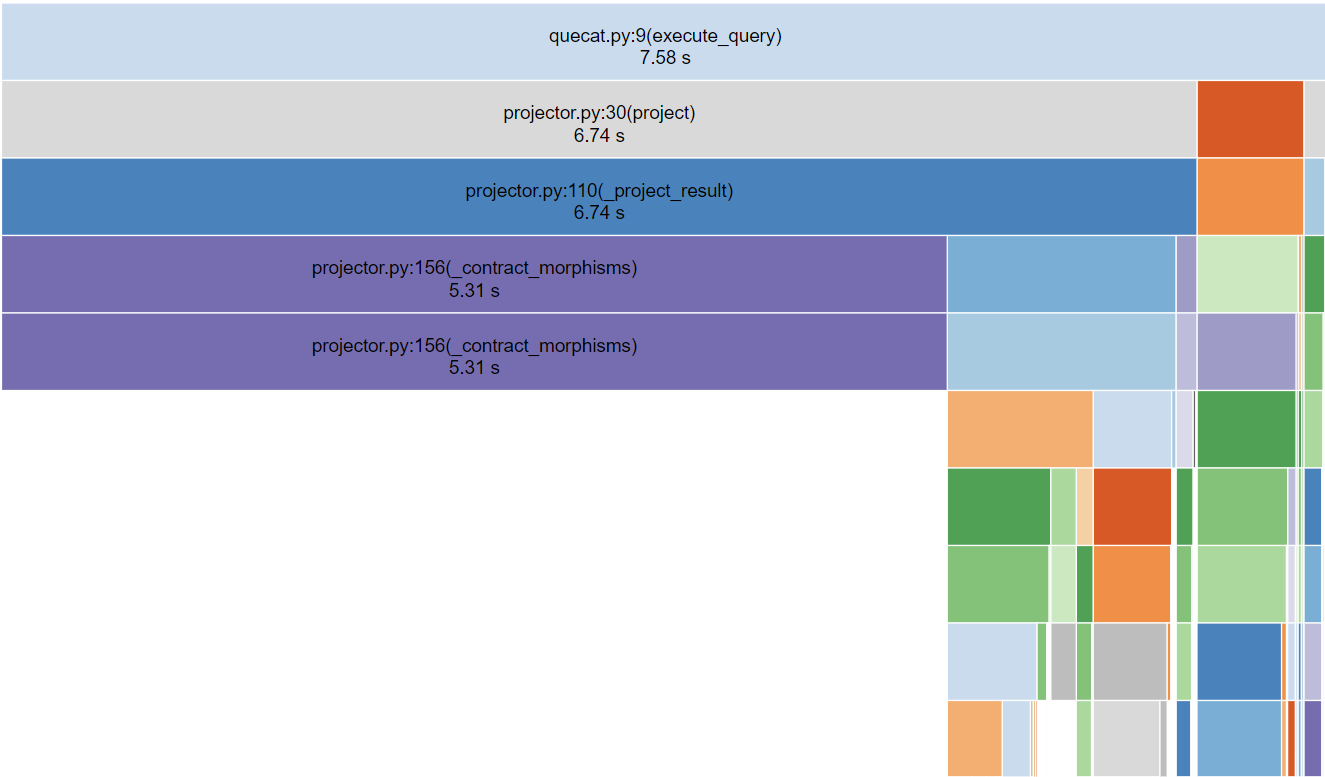
\includegraphics[width=\textwidth]{img/eval-mongodb-profile.png} 
\caption{Profiler data for the single-model MongoDB scenario.}
\label{fig:evalmongodbprofile}
\end{figure}

The reader may be wondering why we did not see this effect of the contractions in~\cref{eval:subsection:postgresql}.
The reason for this can be seen in the structure of the MMQL query itself - the query in this scenario contains the triple \texttt{?order 5/1 ?customerId}, but this compound morphism is contracted into a single base morphism in the \texttt{SELECT} clause.
For that reason, the contractions are needed in this instance, whereas in~\cref{eval:subsection:postgresql}, no such operation was needed due to the structure of the query.

\section{Multi-Model Evaluation}
\label{eval:section:multimodel}

In the previous section, we examined the characteristics of MM-quecat in the context of querying a single database at a time.
However, one of the main benefits of MM-quecat and MMQL is the ability to uniformly query data from multiple databases at a time.
Also, recall that one of the goals for this chapter was to understand the overhead in the context of merging data in a multi-model, which we have not yet done.
This is why this last evaluation scenario is focused on MM-quecat in a multi-model context.

\begin{figure}[ht]
\begin{code}
SELECT {
    ?order id ?orderId ;
        totalPrice ?totalPrice ;
        status ?status ;
        customerName ?customerName ;
        customerSurname ?customerSurname ;
        address ?customerAddress .
}
WHERE {
    ?order 6 ?orderId ;
        7 ?totalPrice ;
        8 ?status ;
        5 ?customer .

    ?customer 2 ?customerName ;
        3 ?customerSurname ;
        4 ?customerAddress .
}
\end{code}
\caption{MMQL query used for multi-model evaluation.}\label{fig:evalmultimodelmmql}
\end{figure}

Recall~\cref{fig:evalcategory}, which shows the schema category used in these evaluations.
In this scenario, we will finally be using the entire schema category.
The MMQL query in~\cref{fig:evalmultimodelmmql} selects data for each order from MongoDB, while also selecting customer data from PostgreSQL and joining the data based on the customer ID stored with the orders.

As this is a multi-model scenario, we will be running queries in both PostgreSQL and MongoDB, and their combined elapsed time form the performance baseline.
These baseline queries are the same as in the previous section (i.e. \cref{fig:evalpostgresqlnative} and \cref{fig:evalmongodbnative}), we will just be using both of them at the same time.
We will also not be showing the queries generated by MMQL in this instance, as they are virtually identical to the generated queries in the previous scenarios.

\begin{table}[h!]
\centering
\begin{tabular}{l@{\hspace{1.5cm}} c c}
& \textbf{Native Queries} & \textbf{MM-evocat} \\
\midrule
Elapsed Time & 46ms & 19209ms \\
Slowdown & 1x & 417x \\
\bottomrule
\end{tabular}
\caption{Average query time measurements for the multi-model scenario.}\label{table:evalmultimodelresults}
\end{table}

The results for this final scenario are shown in~\cref{table:evalmultimodelresults}.
We can see that the native queries combined took approximately 46 milliseconds on average, whereas MM-evocat finished its work in around 19 seconds.

\begin{figure}[h]
\centering
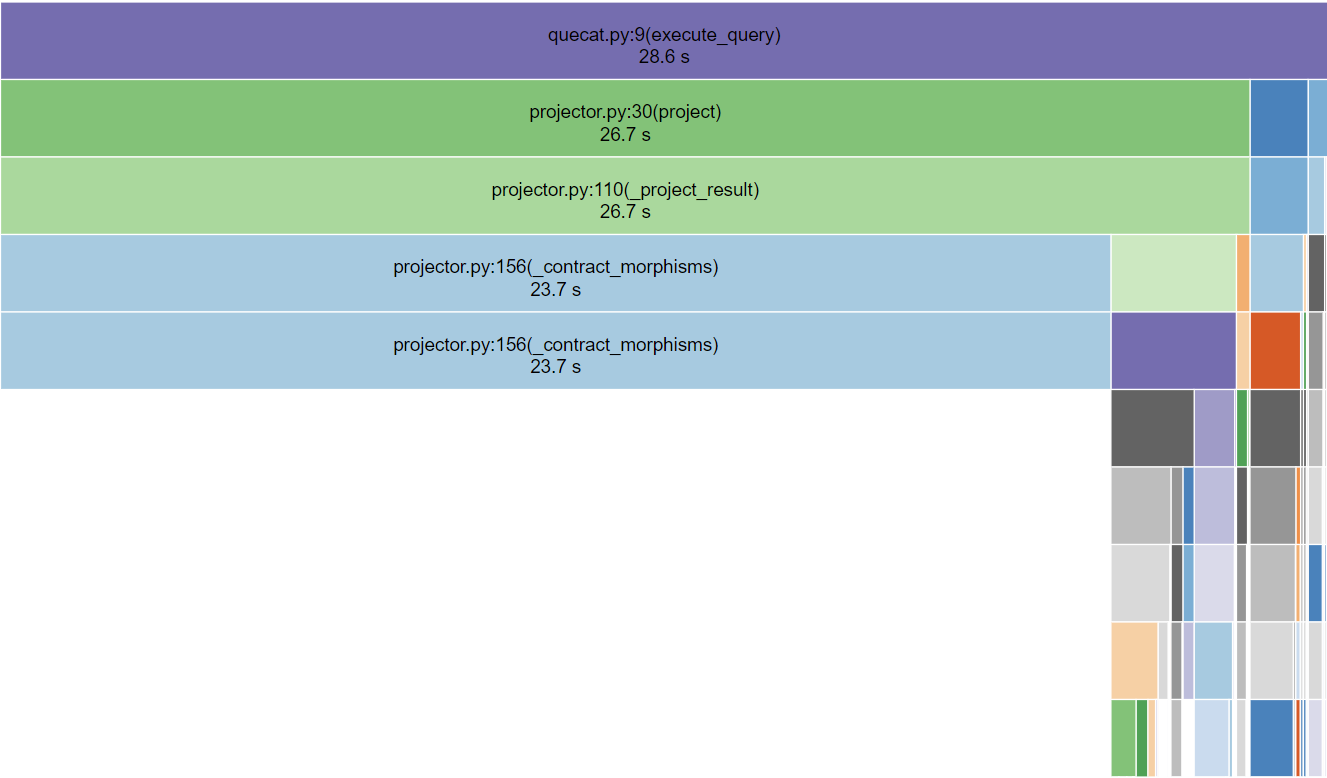
\includegraphics[width=\textwidth]{img/eval-multimodel-profile.png} 
\caption{Profiler data for the multi-model scenario.}
\label{fig:evalmultimodelprofile}
\end{figure}

Examining the profiler data shown in~\cref{fig:evalmultimodelprofile}, we can see a similar image as in~\cref{eval:subsection:mongodb}.
Again, the vast majority of the query execution time is spent on instance morphism contraction, this time over 80\%.
In this instance, the fraction of time spent on contractions is higher, because the query itself also has more contractions to perform.
While the customer ID is not being retrieved this time, all other customer properties are, leading to additional contractions needing to be done.
This, along with the combined volume of data from both databases, explains the increase in query execution time.
Again, as discussed in~\cref{eval:subsection:mongodb}, perhaps there exist more optimized ways of doing the instance morphism contractions, which would improve the overall query performance dramatically.

In addition, we can see that the merging process between the two models does not take a significant amount of time, at least compared to the effort required to perform morphism contractions.
This makes sense, as the merging process does not need to process that much data if the joining object has a simple enough identifier, which is used for the join.
Therefore future efforts in improving the querying performance should not focus on the merging algorithm, but rather on the contraction process (and the projection in general).
In other words, for queries whose projection is trivial, performance improvements are likely to be most effective in the network communication between MM-evocat and MM-quecat, whereas for queries with non-trivial projection, improvements to the morphism contraction will yield the most benefit.


\chapter*{Conclusion}
\addcontentsline{toc}{chapter}{Conclusion}

Multi-model data is a very complex domain with many unsolved problems and much additional research needed, as the reader is surely aware after reading this thesis.
This is especially true for the problem of unified querying of multi-model data, for which no widely usable proposals exist at the time of writing of this thesis, with the vast majority of existing multi-model querying solutions necessitating the knowledge of the specifics of each model involved.
Despite these challenges, in this thesis we worked towards creating one of the first proposals for a unified multi-model querying approach, as we believe that enabling the formation of multi-model queries in a model-agnostic way has massive potential upsides.

To this end, we first introduced the unified multi-model data representation~\cite{one_model}\cite{unified_representation} which we based our efforts on.
Following this, we examined the existing field of graph query languages, as a category may be thought of as a directed multigraph, and selected SPARQL as the prime candidate for adaption to a categorical domain.
We then proposed MMQL, a categorical multi-model query language which given the aforementioned unified categorical data representation, allows users to query across multiple models and databases in a unified, model- and database-agnostic fashion.
In addition to introducing all MMQL concepts together with concrete query examples, we also provided a full formal grammar for this proposed query language.
The main characteristics of MMQL include strong expressiveness in terms of matching graph patterns, familiarity thanks to structural similarities to SPARQL, and leveraging the power of the categorical representation to form elegant graph traversals.

A query language is nothing without the supporting algorithms necessary for its implementation.
For this reason, following the design of MMQL, we also proposed an approach for the implementation of MMQL for multi-model, multi-database scenarios potentially involving data redundancy.
The main accomplishment of our proposed approach is the fact that it can be decomposed into clear, well-defined steps, whose composition forms the whole implementation algorithm.
Since this is the first such approach designed, we focused our design on comprehensibility and simplicity, discussing additional complexities along the way.
During our presentation of our proposed approach for implementing MMQL, we made a special effort to point out any flaws or limitations of our approach, as this will allow further work on this subject to iterate upon our solution.

Following the lengthy design chapters about MMQL and its supporting algorithms, we put our designs to the test by creating a proof-of-concept implementation of MMQL called MM-quecat.
This implementation is limited in scope by the amount of time and work required to propose the entire approach, as well as by constraints placed upon it due to the dependence on another piece of software called MM-evocat, which is in active development, and not all of its required features are finished.
Despite this, MM-quecat serves its purpose as a verification of the validity of our process, functioning as a unified query solution for a subset of MMQL for the PostgreSQL and MongoDB databases.
Although we present MM-quecat in this thesis as it exists in its current state, its feature set will continue to evolve in the future, as the author of this thesis is the co-author of a not-yet-published demo paper showcasing MM-quecat and its unified multi-model querying capabilities, which we are excited to share with the wider multi-model data community.
Related to this, we also presented our proposal for how a graphical query tool for MMQL may look like as part of MM-quecat, demonstrating the final product we will be striving for with our future academic endeavors.

In order to properly evaluate the weaknesses and limitations of our approach, we also performed a handful of experimental evaluations of MM-quecat in an experiment involving PostgreSQL and MongoDB.
We acknowledge that performance is key in the world of multi-model data, but achieving near-native performance is simply too ambitious for an approach with little to no previous related work to support it.
For this reason, we collected query execution time data as well as profiler data during the experiments, and we discussed their implications for our approach.

Overall, we feel that we accomplished all goals which we outlined in the introduction of this thesis, having proposed an innovative approach for unified multi-model querying complete with our own query language called MMQL, laying the groundwork for future research.

\chapter*{Future Work}
\addcontentsline{toc}{chapter}{Future Work}

While presenting MMQL, we provided a full formal grammar, discussed its features, and we showed a comparison of its feature set to existing single-model query languages.
However, we believe that a more formal analysis and verification of the language may be desirable, in order to formally express the capabilities and limitations of MMQL.
Similarly, MMQL may be further extended with features like more aggregation or filtering options, together with additional data types.

When it comes to our proposed MMQL implementation approach, we mentioned a number of open problems in the world of multi-model data which require further study.
More work is needed in the area of multi-model query planning, as there are limited academic resources on this matter, and existing multi-model query planners within polystores do not fit neatly into our problem domain, as they do not take into considerations many variables relevant to our approach.
Together with multi-model query planning, we also mentioned the problem of multi-model join ordering, which also lacks robust and general solutions.

When it comes to the MMQL implementation approach proposed in this thesis, we acknowledge that it has many limitations and weaknesses, which we discussed at great length in various chapters.
Perhaps the largest one of them all is performance, and with performance and scalability often being the driving force behind using multiple data models to begin with, we recognize the need for more optimal versions of algorithms we proposed, possibly using some or all of the optimizations we discussed along the way.
There is room for optimization in almost all areas of the proposed approach, from ensuring that the generated native queries are as optimal as possible, to optimizing the manipulation of categorical data in order to minimize the overhead introduced.
In general, the goal for unified multi-model querying in the future should be to achieve near-native performance when compared to individual database systems while preserving the benefits of unified querying.

Lastly, our MMQL implementation called MM-quecat is purely experimental in nature, and it does not contain all MMQL features for various reasons outlined in this thesis.
In order to bring MM-quecat closer to real-world applicability, we will continue to improve and enhance its implementation as part of our future research efforts.
Coupled with this, we believe that a graphical query tool would be highly beneficial for the end user experience, which is why we are also working on the user interface part of MM-quecat, which we hope to demonstrate to the academic community in the coming months.


%%% Bibliography
%%% Bibliography (literature used as a source)
%%%
%%% We employ bibTeX to construct the bibliography. It processes
%%% citations in the text (e.g., the \cite{...} macro) and looks up
%%% relevant entries in the bibliography.bib file.
%%%
%%% The \bibliographystyle command selects, which style will be used
%%% for references from the text. The argument in curly brackets is
%%% the name of the corresponding style file (*.bst). Both styles
%%% mentioned in this template are included in LaTeX distributions.

% \bibliographystyle{plainnat}    %% Author (year)
\bibliographystyle{unsrt}     %% [number]

\renewcommand{\bibname}{Bibliography}

%%% Generate the bibliography. Beware that if you cited no works,
%%% the empty list will be omitted completely.

\bibliography{bibliography}

%%% If case you prefer to write the bibliography manually (without bibTeX),
%%% you can use the following. Please follow the ISO 690 standard and
%%% citation conventions of your field of research.

% \begin{thebibliography}{99}
%
% \bibitem{lamport94}
%   {\sc Lamport,} Leslie.
%   \emph{\LaTeX: A Document Preparation System}.
%   2nd edition.
%   Massachusetts: Addison Wesley, 1994.
%   ISBN 0-201-52983-1.
%
% \end{thebibliography}


%%% Figures used in the thesis (consider if this is needed)
\listoffigures

%%% Tables used in the thesis (consider if this is needed)
%%% In mathematical theses, it could be better to move the list of tables to the beginning of the thesis.
\listoftables

%%% Abbreviations used in the thesis, if any, including their explanation
%%% In mathematical theses, it could be better to move the list of abbreviations to the beginning of the thesis.
\chapwithtoc{List of Abbreviations}

\textbf{ACID} Atomicity, Consistency, Isolation, Durability \\
\textbf{API} Application Programming Interface \\
\textbf{AST} Abstract Syntax Tree \\
\textbf{CPU} Central Processing Unit \\
\textbf{CQL} Categorical Query Language \\
\textbf{ER} Entity Relationship diagram \\
\textbf{HTTP} Hypertext Transfer Protocol \\
\textbf{IRI} Internationalized Resource Identifier \\
\textbf{JSON} JavaScript Object Notation \\
\textbf{MMQL} Multi-Model Query Language \\
\textbf{OLAP} Online Analytical Processing \\
\textbf{OLTP} Online Transaction Processing \\
\textbf{ORM} Object-Relational Mapping \\
\textbf{RDF} Resource Description Framework \\
\textbf{REST} Representational State Transfer \\
\textbf{SPARQL} SPARQL Protocol and RDF Query Language \\
\textbf{SSD} Solid-State Drive \\
\textbf{SQL} Structured Query Language \\
\textbf{UI} User Interface \\
\textbf{XML} Extensible Markup Language

%%% Attachments to the master thesis, if any. Each attachment must be
%%% referred to at least once from the text of the thesis. Attachments
%%% are numbered.
%%%
%%% The printed version should preferably contain attachments, which can be
%%% read (additional tables and charts, supplementary text, examples of
%%% program output, etc.). The electronic version is more suited for attachments
%%% which will likely be used in an electronic form rather than read (program
%%% source code, data files, interactive charts, etc.). Electronic attachments
%%% should be uploaded to SIS and optionally also included in the thesis on a~CD/DVD.
%%% Allowed file formats are specified in provision of the rector no. 72/2017.
\appendix
\chapter{Attachments}

\section{MMQL Grammar}
\label{attachment:grammar}

This attachment contains a full formal grammar of MMQL, which was used to generate a parser for the query language.
The grammar is in the G4 format.

\begin{code}
grammar MMQL;

query: selectQuery EOF;

selectQuery: selectClause fromClause? whereClause solutionModifier;

subSelect: selectQuery;

selectClause: 'SELECT' selectGraphPattern;

selectGraphPattern: '{' selectTriples? '}';

fromClause: 'FROM' SCHEMA_IDENTIFIER;

whereClause: 'WHERE'? groupGraphPattern;

solutionModifier: orderClause? limitOffsetClauses?;

limitOffsetClauses: (
		limitClause offsetClause?
		| offsetClause limitClause?
	);

orderClause: 'ORDER' 'BY' orderCondition+;

orderCondition: (( 'ASC' | 'DESC') brackettedExpression)
	| ( constraint | var_);

limitClause: 'LIMIT' INTEGER;

offsetClause: 'OFFSET' INTEGER;

groupGraphPattern:
	'{' (subSelect | (triplesBlock? (
		(graphPatternNotTriples | filter_) '.'? triplesBlock?
	)*)) '}';

triplesBlock: triplesSameSubject ( '.' triplesBlock?)?;

graphPatternNotTriples:
	optionalGraphPattern
	| groupOrUnionGraphPattern
	| inlineData;

optionalGraphPattern: 'OPTIONAL' groupGraphPattern;

groupOrUnionGraphPattern:
	groupGraphPattern (('UNION' | 'MINUS') groupGraphPattern)*;

inlineData: 'VALUES' dataBlock;

dataBlock: var_ '{' dataBlockValue* '}';

dataBlockValue: numericLiteral
	| booleanLiteral
	| string_;

filter_: 'FILTER' constraint;

constraint: brackettedExpression;

selectTriples: triplesSameSubject ( '.' selectTriples?)?;

triplesSameSubject: varOrTerm propertyListNotEmpty;

propertyListNotEmpty: verb objectList ( ';' ( verb objectList)?)*;

propertyList: propertyListNotEmpty?;

objectList: object_ ( ',' object_)*;

object_: graphNode;

verb: schemaMorphismOrPath;

schemaMorphismOrPath: pathAlternative;

pathAlternative: pathSequence ( '|' pathSequence )*;

pathSequence: pathWithMod ( '/' pathWithMod )*;

pathWithMod: pathPrimary pathMod?;

pathMod: '?' | '*' | '+';

pathPrimary: schemaMorphism | ( '(' schemaMorphismOrPath ')' ) ;

schemaMorphism: primaryMorphism | dualMorphism;

primaryMorphism: SCHEMA_MORPHISM;

dualMorphism: '-' primaryMorphism;

graphNode: varOrTerm ( 'AS' var_)?;

varOrTerm: var_ | constantTerm | aggregationTerm;

var_: VAR1 | VAR2;

constantTerm:
	numericLiteral
	| booleanLiteral
	| string_
	| blankNode
	| NIL;

aggregationTerm:
	aggregationFunc '(' (distinctModifier)? var_ ')';

distinctModifier:
	'DISTINCT';

aggregationFunc:
	'COUNT'
	| 'SUM'
	| 'AVG'
	| 'MIN'
	| 'MAX';

expression: conditionalOrExpression;

conditionalOrExpression:
	conditionalAndExpression ('||' conditionalAndExpression)*;

conditionalAndExpression: valueLogical ( '&&' valueLogical)*;

valueLogical: relationalExpression;

relationalExpression:
	expressionPart (
		'=' expressionPart
		| '!=' expressionPart
		| '<' expressionPart
		| '>' expressionPart
		| '<=' expressionPart
		| '>=' expressionPart
	)?;

expressionPart: primaryExpression;

primaryExpression:
	brackettedExpression
	| numericLiteral
	| booleanLiteral
	| string_
	| varOrTerm;

brackettedExpression: '(' expression ')';

numericLiteral:
	numericLiteralUnsigned
	| numericLiteralPositive
	| numericLiteralNegative;

numericLiteralUnsigned: INTEGER | DECIMAL | DOUBLE;

numericLiteralPositive:
	INTEGER_POSITIVE
	| DECIMAL_POSITIVE
	| DOUBLE_POSITIVE;

numericLiteralNegative:
	INTEGER_NEGATIVE
	| DECIMAL_NEGATIVE
	| DOUBLE_NEGATIVE;

booleanLiteral: 'true' | 'false';

string_:
	STRING_LITERAL1
	| STRING_LITERAL2;

blankNode: BLANK_NODE_LABEL | ANON;

// LEXER RULES

SCHEMA_MORPHISM: (PN_CHARS)+;

SCHEMA_IDENTIFIER: (PN_CHARS)+;

BLANK_NODE_LABEL: '_:' PN_LOCAL;

VAR1: '?' VARNAME;

VAR2: '$' VARNAME;

INTEGER: DIGIT+;

DECIMAL: DIGIT+ '.' DIGIT* | '.' DIGIT+;

DOUBLE:
	DIGIT+ '.' DIGIT* EXPONENT
	| '.' DIGIT+ EXPONENT
	| DIGIT+ EXPONENT;

INTEGER_POSITIVE: '+' INTEGER;

DECIMAL_POSITIVE: '+' DECIMAL;

DOUBLE_POSITIVE: '+' DOUBLE;

INTEGER_NEGATIVE: '-' INTEGER;

DECIMAL_NEGATIVE: '-' DECIMAL;

DOUBLE_NEGATIVE: '-' DOUBLE;

EXPONENT: ('e' | 'E') ('+' | '-')? DIGIT+;

STRING_LITERAL1:
	'\'' (
		~('\u0027' | '\u005C' | '\u000A' | '\u000D') | ECHAR
	)* '\'';

STRING_LITERAL2:
	'"' (
		~('\u0022' | '\u005C' | '\u000A' | '\u000D') | ECHAR
	)* '"';

STRING_LITERAL_LONG1:
	'\'\'\'' (
		( '\'' | '\'\'')? (~('\'' | '\\') | ECHAR)
	)* '\'\'\'';

STRING_LITERAL_LONG2:
	'"""' (
		( '"' | '""')? ( ~('\'' | '\\') | ECHAR)
	)* '"""';

ECHAR: '\\' ('t' | 'b' | 'n' | 'r' | 'f' | '"' | '\'');

NIL: '(' WS* ')';

ANON: '[' WS* ']';

PN_CHARS_U: PN_CHARS_BASE | '_';

VARNAME: (PN_CHARS_U | DIGIT) (
		PN_CHARS_U
		| DIGIT
		| '\u00B7'
		| ('\u0300' ..'\u036F')
		| ('\u203F' ..'\u2040')
	)*;

fragment PN_CHARS:
	PN_CHARS_U
	| '-'
	| DIGIT;

PN_PREFIX: PN_CHARS_BASE ((PN_CHARS | '.')* PN_CHARS)?;

PN_LOCAL: ( PN_CHARS_U | DIGIT) ((PN_CHARS | '.')* PN_CHARS)?;

fragment PN_CHARS_BASE:
	'A' ..'Z'
	| 'a' ..'z'
	| '\u00C0' ..'\u00D6'
	| '\u00D8' ..'\u00F6'
	| '\u00F8' ..'\u02FF'
	| '\u0370' ..'\u037D'
	| '\u037F' ..'\u1FFF'
	| '\u200C' ..'\u200D'
	| '\u2070' ..'\u218F'
	| '\u2C00' ..'\u2FEF'
	| '\u3001' ..'\uD7FF'
	| '\uF900' ..'\uFDCF'
	| '\uFDF0' ..'\uFFFD';

fragment DIGIT: '0' ..'9';

WS: (' ' | '\t' | '\n' | '\r')+ -> skip;
\end{code}
\pagebreak
\section{Query Planner Information in PostgreSQL}
\label{attachment:plannerpostgresql}

Below, we can see the query planner information exposed by the \texttt{EXPLAIN} statement in PostgreSQL for a simple query selecting all theaters whose primary identifier is greater than a constant number.
We can see that the set of information returned contains a full description of the winning query plan, complete with estimated costs for each step of the plan, and the information about which indexes the query is using.

\begin{code}
EXPLAIN (FORMAT YAML) SELECT * FROM theaters WHERE id > 1010;

          QUERY PLAN
-------------------------------
 - Plan: 
    Node Type: "Bitmap Heap Scan"
    Parallel Aware: false
    Async Capable: false
    Relation Name: "theaters"
    Alias: "theaters"
    Startup Cost: 6.34
    Total Cost: 19.88
    Plan Rows: 283
    Plan Width: 68
    Recheck Cond: "(id > 1010)"
    Plans: 
      - Node Type: "Bitmap Index Scan"
        Parent Relationship: "Outer"
        Parallel Aware: false
        Async Capable: false
        Index Name: "theaters_pkey"
        Startup Cost: 0.00
        Total Cost: 6.27
        Plan Rows: 283
        Plan Width: 0
        Index Cond: "(id > 1010)"   
(1 row)
\end{code}

\pagebreak
\section{Query Planner Information in MongoDB}
\label{attachment:explainmongodb}

Below, we can see two sets of query planner information returned by MongoDB. The first output shown calls the \texttt{explain()} function with the default \texttt{queryPlanner} mode, which does not execute the query, but also does not include cost or the approximate result size.

The second output uses the \texttt{executionStats} mode, which executes the query, and subsequently returns query plan information including cost information (represented in the form of the \texttt{works} property signifying units of work required).

\begin{code}
db.theaters.explain().find({ theaterId: { $gt: 1020 } });
{
  "queryPlanner" : {
    "plannerVersion" : 1,
    "namespace" : "sample_mflix.theaters",
    "indexFilterSet" : false,
    "parsedQuery" : {
      "theaterId" : {
        "$gt" : 1020
      }
    },
    "winningPlan" : {
      "stage" : "FETCH",
      "inputStage" : {
        "stage" : "IXSCAN",
        "keyPattern" : {
          "theaterId" : 1
        },
        "indexName" : "theaterId_1",
        "isMultiKey" : false,
        "multiKeyPaths" : {
          "theaterId" : [ ]
        },
        "isUnique" : true,
        "isSparse" : false,
        "isPartial" : false,
        "indexVersion" : 2,
        "direction" : "forward",
        "indexBounds" : {
          "theaterId" : [
            "(1020.0, inf.0]"
          ]
        }
      }
    },
    "rejectedPlans" : [ ]
  }
}
\end{code}

\pagebreak

\begin{code}
db.theaters.explain({verbosity: "executionStats"}).find(
    {theaterId: {$gt: 1020}}
);
{
  "queryPlanner" : {
    "plannerVersion" : 1,
    "namespace" : "sample_mflix.theaters",
    "indexFilterSet" : false,
    "parsedQuery" : {
      "theaterId" : {
        "$gt" : 1020
      }
    },
    "winningPlan" : {
      "stage" : "FETCH",
      "inputStage" : {
        "stage" : "IXSCAN",
        "keyPattern" : {
          "theaterId" : 1
        },
        "indexName" : "theaterId_1",
        "isMultiKey" : false,
        "multiKeyPaths" : {
          "theaterId" : [ ]
        },
        "isUnique" : true,
        "isSparse" : false,
        "isPartial" : false,
        "indexVersion" : 2,
        "direction" : "forward",
        "indexBounds" : {
          "theaterId" : [
            "(1020.0, inf.0]"
          ]
        }
      }
    },
    "rejectedPlans" : [ ]
  },
  "executionStats" : {
    "executionSuccess" : true,
    "nReturned" : 861,
    "executionTimeMillis" : 1,
    "totalKeysExamined" : 861,
    "totalDocsExamined" : 861,
    "executionStages" : {
      "stage" : "FETCH",
      "nReturned" : 861,
      "executionTimeMillisEstimate" : 0,
      "works" : 862,
      "advanced" : 861,
      "needTime" : 0,
      "needYield" : 0,
      "saveState" : 6,
      "restoreState" : 6,
      "isEOF" : 1,
      "invalidates" : 0,
      "docsExamined" : 861,
      "alreadyHasObj" : 0,
      "inputStage" : {
        "stage" : "IXSCAN",
        "nReturned" : 861,
        "executionTimeMillisEstimate" : 0,
        "works" : 862,
        "advanced" : 861,
        "needTime" : 0,
        "needYield" : 0,
        "saveState" : 6,
        "restoreState" : 6,
        "isEOF" : 1,
        "invalidates" : 0,
        "keyPattern" : {
          "theaterId" : 1
        },
        "indexName" : "theaterId_1",
        "isMultiKey" : false,
        "multiKeyPaths" : {
          "theaterId" : [ ]
        },
        "isUnique" : true,
        "isSparse" : false,
        "isPartial" : false,
        "indexVersion" : 2,
        "direction" : "forward",
        "indexBounds" : {
          "theaterId" : [
            "(1020.0, inf.0]"
          ]
        },
        "keysExamined" : 861,
        "seeks" : 1,
        "dupsTested" : 0,
        "dupsDropped" : 0,
        "seenInvalidated" : 0
      }
    },
    "allPlansExecution" : [ ]
  }
}
\end{code}

\pagebreak
\section{Query Planner Information in Neo4j}
\label{attachment:plannerneo4j}

Below, we can see the query planner information exposed by the \texttt{EXPLAIN} statement in Neo4j for a simple query matching nodes with the \texttt{name} property set to ``Tom Hanks''.
For each stage in the query plan, the estimated number of rows is returned.

\begin{code}
{
  "query": {
    "text": "EXPLAIN MATCH (tom {name: \"Tom Hanks\"}) RETURN tom",
    "parameters": {}
  },
  "queryType": "r",
  "counters": {
    "_stats": {
      "nodesCreated": 0,
      "nodesDeleted": 0,
      "relationshipsCreated": 0,
      "relationshipsDeleted": 0,
      "propertiesSet": 0,
      "labelsAdded": 0,
      "labelsRemoved": 0,
      "indexesAdded": 0,
      "indexesRemoved": 0,
      "constraintsAdded": 0,
      "constraintsRemoved": 0
    },
    "_systemUpdates": 0
  },
  "updateStatistics": {
    "_stats": {
      "nodesCreated": 0,
      "nodesDeleted": 0,
      "relationshipsCreated": 0,
      "relationshipsDeleted": 0,
      "propertiesSet": 0,
      "labelsAdded": 0,
      "labelsRemoved": 0,
      "indexesAdded": 0,
      "indexesRemoved": 0,
      "constraintsAdded": 0,
      "constraintsRemoved": 0
    },
    "_systemUpdates": 0
  },
  "plan": {
    "operatorType": "ProduceResults@neo4j",
    "identifiers": [
      "tom"
    ],
    "arguments": {
      "planner-impl": "IDP",
      "Details": "tom",
      "PipelineInfo": "Fused in Pipeline 0",
      "planner-version": "4.4",
      "runtime-version": "4.4",
      "runtime": "PIPELINED",
      "runtime-impl": "PIPELINED",
      "version": "CYPHER 4.4",
      "EstimatedRows": 17,
      "planner": "COST"
    },
    "children": [
      {
        "operatorType": "Filter@neo4j",
        "identifiers": [
          "tom"
        ],
        "arguments": {
          "Details": "tom.name = $autostring_0",
          "EstimatedRows": 17,
          "PipelineInfo": "Fused in Pipeline 0"
        },
        "children": [
          {
            "operatorType": "AllNodesScan@neo4j",
            "identifiers": [
              "tom"
            ],
            "arguments": {
              "Details": "tom",
              "EstimatedRows": 340,
              "PipelineInfo": "Fused in Pipeline 0"
            },
            "children": []
          }
        ]
      }
    ]
  },
  "profile": false,
  "notifications": [],
  "server": {
    "address": "localhost:7687",
    "version": "Neo4j/4.4.5",
    "agent": "Neo4j/4.4.5",
    "protocolVersion": 4.4
  },
  "resultConsumedAfter": {
    "low": 0,
    "high": 0
  },
  "resultAvailableAfter": {
    "low": 0,
    "high": 0
  },
  "database": {
    "name": "neo4j"
  }
}
\end{code}


\openright
\end{document}
